\documentclass[aspectratio=43]{beamer}
\usetheme{CCNU}
%\usefonttheme[onlymath]{serif}

\usepackage{slashed}
\usepackage{datetime}
%\usepackage{slidesphysics}
\graphicspath{{../img/}}

\usepackage{media9}
\addmediapath{./Movies/}

\usepackage{multimedia}

\usepackage{hyperref}
\usepackage{cancel}
% \hypersetup{colorlinks=true, 
%     linkcolor=blue,          % color of internal links (change box color with linkbordercolor)
%     citecolor=black,        % color of links to bibliography
%     filecolor=black,      % color of file links
%     urlcolor=blue    }
% \usepackage{deflamb}
% \usepackage{color, colortbl}
% \usepackage{tikz}
%\usepackage{userdef}
\usepackage[absolute,overlay]{textpos}
\def\Put(#1,#2)#3{\leavevmode\makebox(0,0){\put(#1,#2){#3}}}

\def\mydate{\leavevmode\hbox{\the\year-\twodigits\month-\twodigits\day}}
\def\twodigits#1{\ifnum#1<10 0\fi\the#1}

\newcommand\Wider[2][3em]{%
\makebox[\linewidth][c]{%
  \begin{minipage}{\dimexpr\textwidth+#1\relax}
  \raggedright
  \centering#2
  \end{minipage}%
  }%
}


% Uncomment one of these to show notes in the compiled presentation
% \setbeameroption{show notes} % Shows notes below slides
% \setbeameroption{show notes on second screen=right} % Shows notes on the second screen


%\def\meetingname{Alicia Garrido Peña. PhD thesis Presentation}


\def\meetingname{Alicia Garrido Peña. PhD thesis Presentation}

\title[\meetingname]{Characterization of the sequential nature of neuronal dynamics: \\Experimental recordings, computational models and novel stimulation neurotechnologies}
\author[A. Garrido-Peña]{Alicia Garrido Peña\\Advisor: Pablo Varona Martínez}
\newcommand{\advisorname}{Pablo Varona Martínez}
% \institute[Michigan]{}
\institute[EPS-UAM]{Escuela Politécnica Superior.\\ Universidad Autónoma de Madrid}
\date[\mydate]{\meetingname\\08-11-2024}

\begin{document}
	
% Set up the section page style
\AtBeginSection[]{
	\begin{frame}
		\centering
		\Huge \insertsection
	\end{frame}
}

	
	
\begin{frame}[plain,t]
\titlepage
\end{frame}

%The next statement creates the title page.
\begin{frame}
\frametitle{Contents}
\tableofcontents
\end{frame}
%------------------------------------------------------------
\section{Introduction}
\begin{frame}{Neuroscience}
	\only<1>{\centering\includegraphics[width=0.8\textwidth]{intro/neurosciences.pdf}}

\end{frame}
\begin{frame}{Approach}
	\begin{itemize}
		\item Neurocomputational Perspective
		\item<2-> Bottom-up approach
		\item<5-> Combining electrophysiology\uncover<6->{, computational work} \uncover<7>{and novel neurotechnology.}
	\end{itemize}
	\vfill
	\centering
	\uncover<3-4>{
\includegraphics[width=0.3\textwidth]{intro/ions.pdf}}
	\hspace{30pt}
	\uncover<4-4>{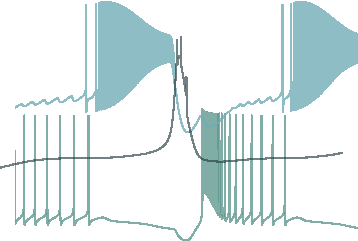
\includegraphics[width=0.4\textwidth]{intro/CPG.pdf}}
	\uncover<3-4>{\\From ionic channels}
	\uncover<4-4>{\hspace{50pt} To minimal circuits}
\end{frame}

\begin{frame}{Neuronal and Networks Dynamics}
	\note{Say if they are recordings and which are those}
	\only<1>{Neuronal electrical activity is often described in terms of the evolution of membrane voltage caused by the flow of ionic channels between the inside and outside of the cell.}
	
	\only<2->{Depending on the channels that constitute the neuron and the circuit it is immersed in, the activity varies.
	\vfill
	\uncover<3->{In terms of the spike waveform:}
	\uncover<3->{\begin{center}
			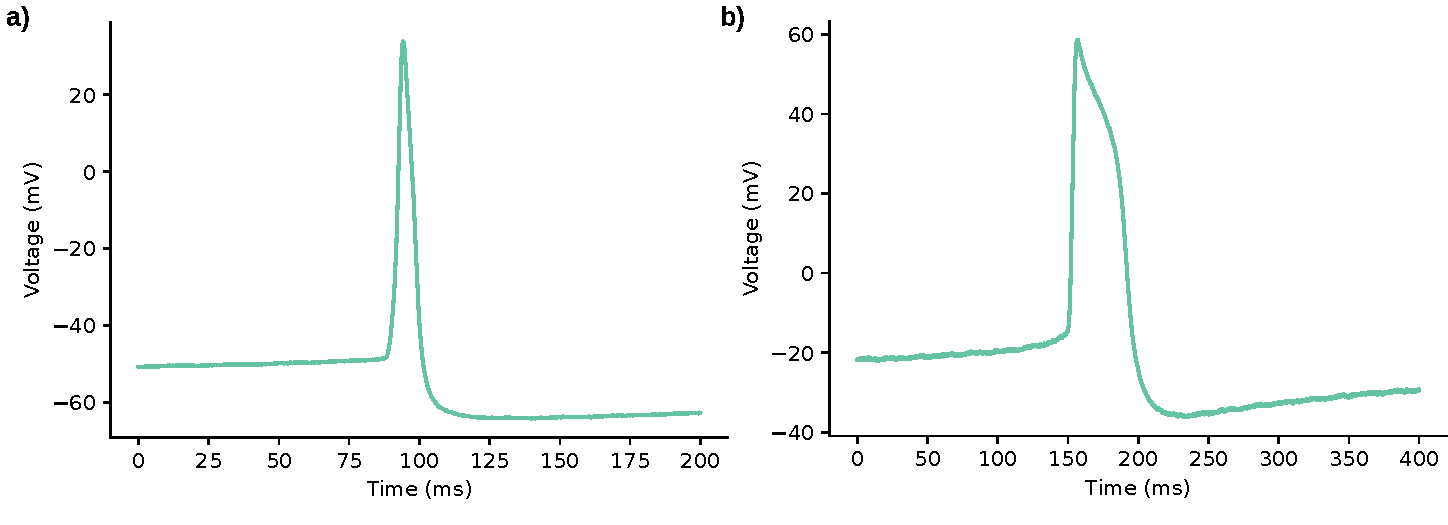
\includegraphics[width=0.7\textwidth]{intro/spike-types.pdf}
	\end{center}}
	
	\uncover<4->{\vfill}
	\uncover<4->{And the type of spiking activity: tonic firing, bursting, etc.}
	\uncover<4->{\begin{center}
			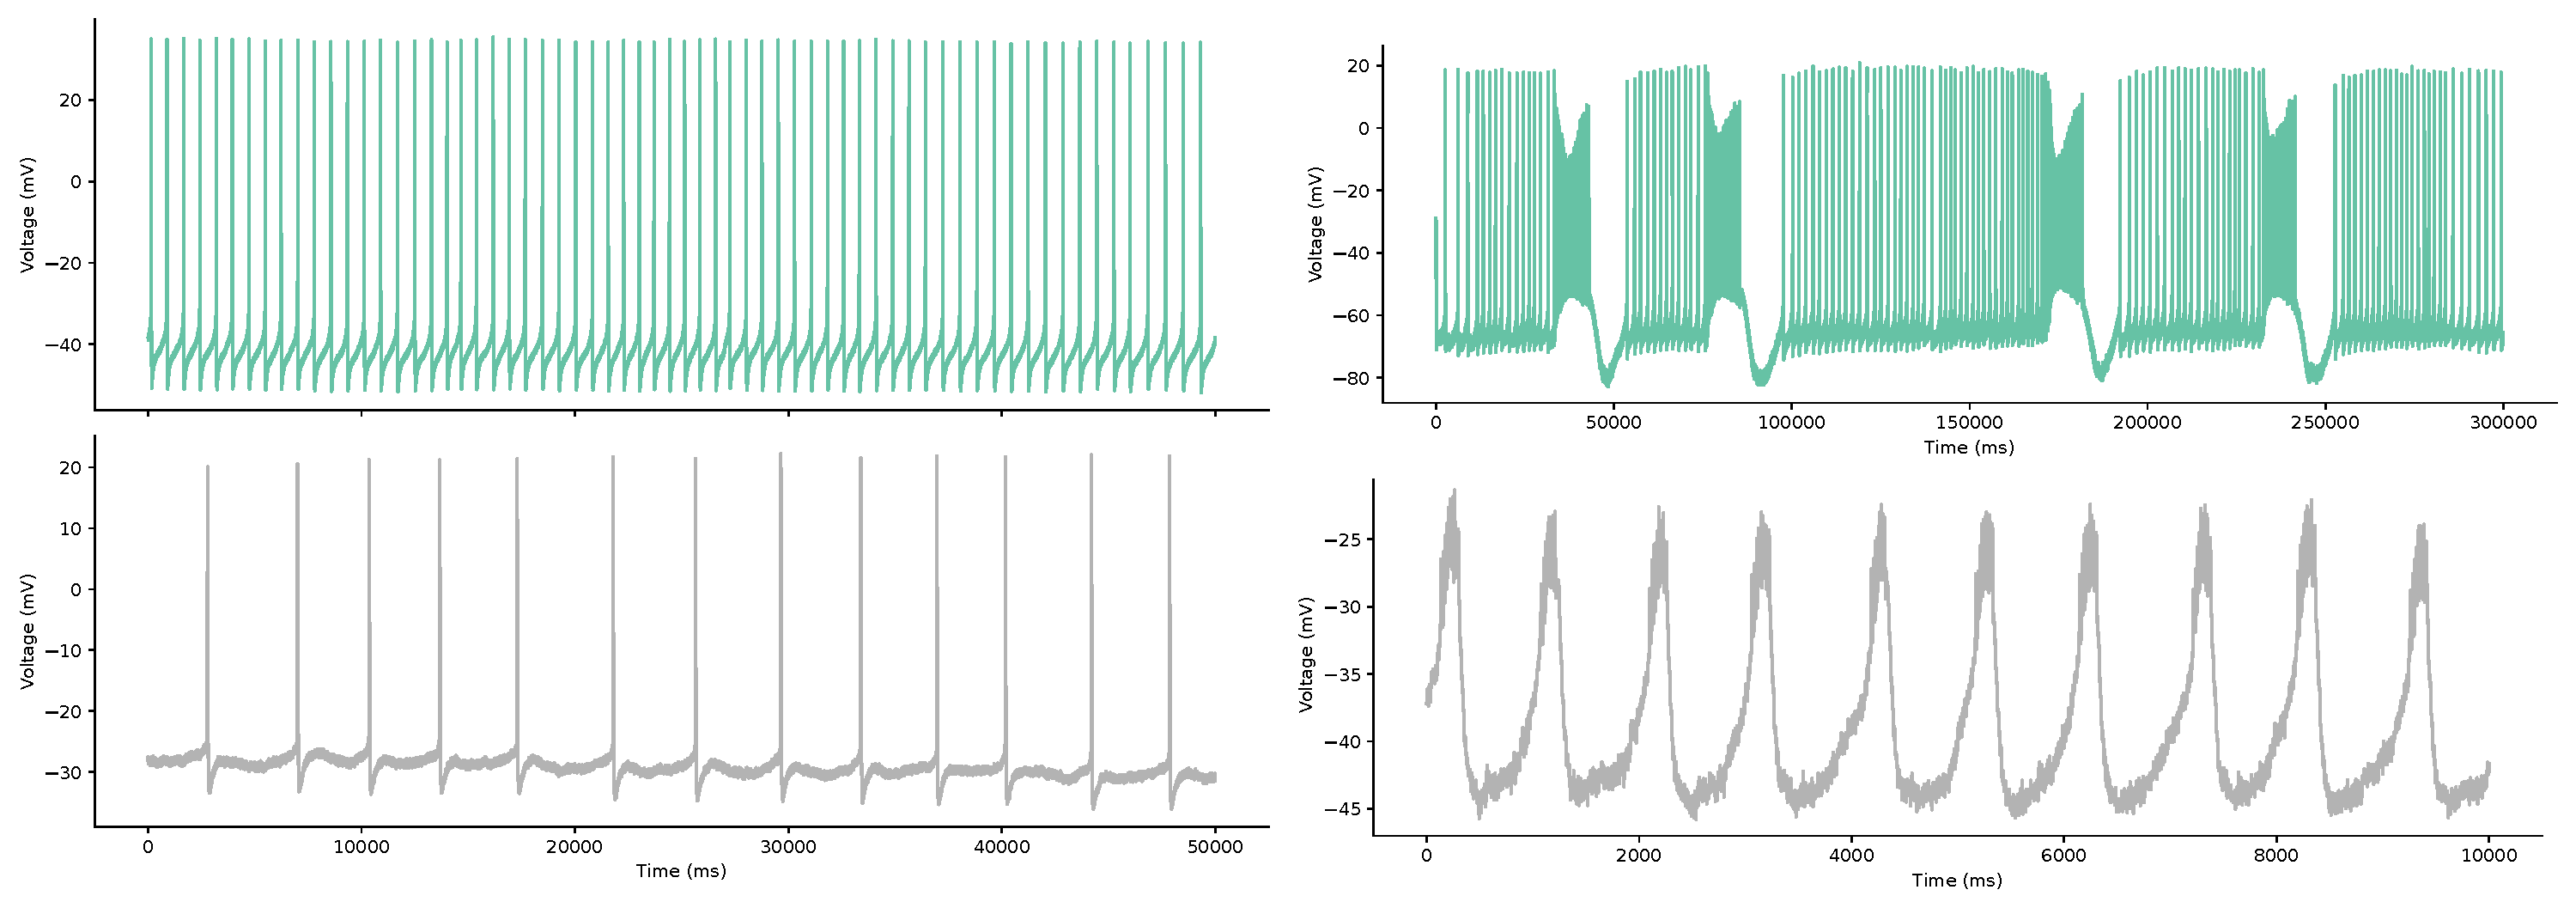
\includegraphics[width=0.8\textwidth]{intro/spike_activity-types.pdf}
			%TODO no se ven los picos zoom?
			\note{Señalar los picos}
	\end{center}}
}
\end{frame}

\begin{frame}{The sequential nature of neural dynamics}
	 \begin{columns}
			\begin{column}{0.6\textwidth}
				\begin{itemize}
					\item<1->{There are sequential processes at different time-scales.} \note{activation of iones and molecules -> dynamics of ions and molecules}
					\item<3->{Many behaviors and actions are governed by sequential processes}
					\item<4->{In humans: Motor control, speech, etc. } %decision making out pq too much para comparar con caracoles.
%					\item<5->{Studying sequential activity at different scales is crucial for a complete comprehension of neural systems.}
					\item<5->{Study of sequential activity might have a crucial role in neural coordination to autonomously establish a balance between the robustness and flexibility required for effective motor function.}
				\end{itemize}
			\end{column}
			\begin{column}{0.45\textwidth}
				\uncover<2->{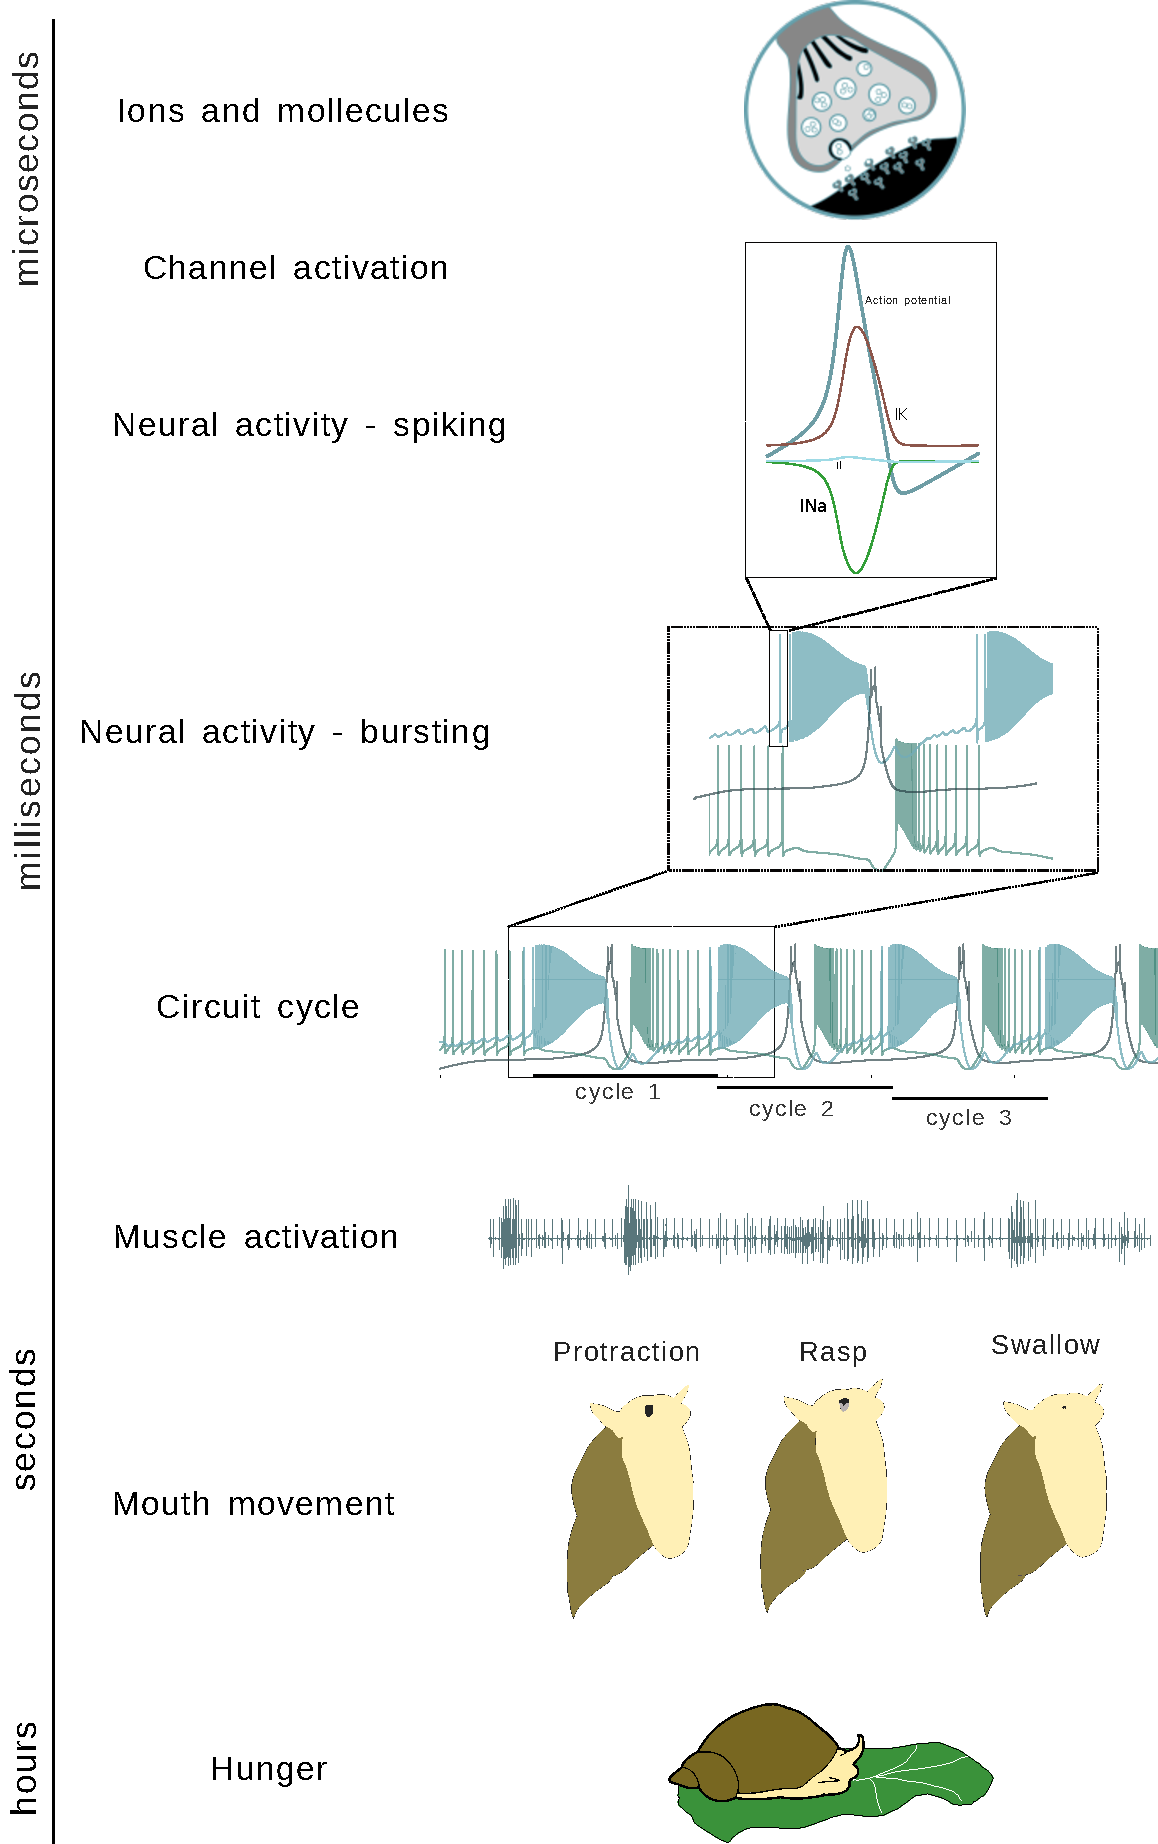
\includegraphics[width=\textwidth]{intro/time scale/time-scale-feeding.pdf}}
			\end{column}
		\end{columns}
	\note{information about the neural system: partial information available form the neural system.
	}
	 
\end{frame}
\begin{frame}{Studying neural dynamics in computational models}
	\only<1-7>{
		\begin{itemize}
			\item<1-7>{Computational models are powerful tools to study neural dynamics}
			\item<2-7>{Advantages}
			\begin{itemize}
				\item<3-7>Full accessibility to the system
				\item<4-7>Detailed reproduction of the living activity
			\end{itemize}
			\item<5-7>{Limitations}
			\begin{itemize}
				\item<6-7>{Restricted variability}
				\item<7>{The description may depend on the information about the living system}
			\end{itemize}
		\end{itemize}
	}
\end{frame}
\begin{frame}{Studying neural dynamics in computational models}

	\only<-1>{
		\textbf{Conductance-based models}
		\uncover<1>{\begin{table}[h!]
			\resizebox{\textwidth}{!}{%
				\begin{tabular}{lccc}
					Voltage equation                                                                 & \multicolumn{3}{c}{$C \frac{dV}{dt} = I - g_K n^4 (V - E_K) - g_{Na} m^3h(V-E_{Na}) - g_L (V-E_L)$}                                                                                                                                  \\ \hline
					& \multicolumn{2}{c}{Activation variables}                                                                                                                              & Inactivation variable                                        \\ \hline
					\multicolumn{1}{c|}{\begin{tabular}[c]{@{}c@{}}gating \\ variables\end{tabular}} & \multicolumn{1}{c|}{$\frac{dm(t)}{dt}=\frac{m_{\infty}(V(t))-m(t)}{\tau_m(V(t))}$} & \multicolumn{1}{c|}{$\frac{dn(t)}{dt}=\frac{n_{\infty}(V(t))-n(t)}{\tau_n(V(t))}$} & $\frac{dh(t)}{dt}=\frac{h_{\infty}(V(t))-h(t)}{\tau_h(V(t))}$ \\ \hline
				\end{tabular}%
			}
		\end{table}
	}
	}

\end{frame}
\begin{frame}{Studying neural dynamics in computational models}

	\only<1-2>{
	\textbf{Conductance-based models}
	\\
	\uncover<1->{By \textbf{different combinations of ionic channels} we can achieve \textbf{different activities and waveform shapes\\\vspace{4pt}}}
	\uncover<2>{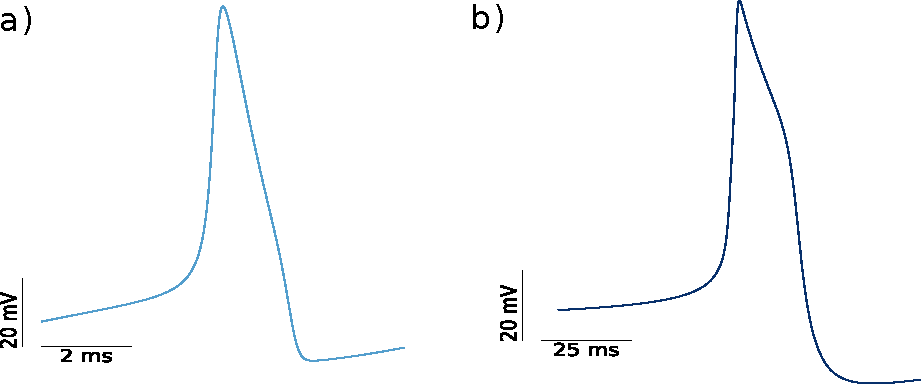
\includegraphics[width=\linewidth]{intro/spike-types model.pdf}
	
	\begin{columns}
		\begin{column}{0.57\textwidth}
			\centering
			\small{Hodgkin and Huxley (1952)}
		\end{column}
		\begin{column}{0.57\textwidth}
			\centering
			\small{Vavoulis et al. (2010)}
		\end{column}
	\end{columns}
	}}
\end{frame}
\begin{frame}{Studying neural dynamics in computational models}

	\textbf{Conductance-based models\\}
	By \textbf{modeling synapses} we can model whole \textbf{circuits} by connecting single modeled neurons.\\
	\uncover<1>{\centering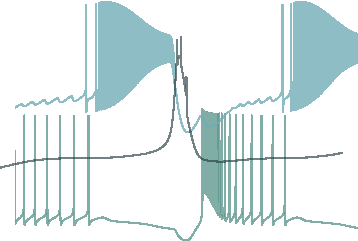
\includegraphics[width=0.7\linewidth]{intro/cpg.pdf}}
	%TODO hacer que aparezca cada modelo de neurona x click.

\end{frame}


\begin{frame}{Vertebrate and invertebrate animal studies}
	\only<1-7>{
	\begin{itemize}
	\item<1->In addition to the well-known vertebrate models, there have been invaluable findings using invertebrates.
	\item<2->There are many universal characteristics of nervous systems and behaviors that can be extrapolated to humans.
	\item<3->Using invertebrates as animal models have different advantages:
		\begin{itemize}
			\item<4->Ease of accessibility to the nervous system.
			\item<5-> Longer survival times of the preparations.
			\item<6-> Ease of breeding and reproduction. 
			\item<7-> Full description of their systems. 
		\end{itemize}
	\end{itemize}
}
\end{frame}
\begin{frame}{Vertebrate and invertebrate animal studies}

		\begin{columns}[t]
			\column{0.4\textwidth}
			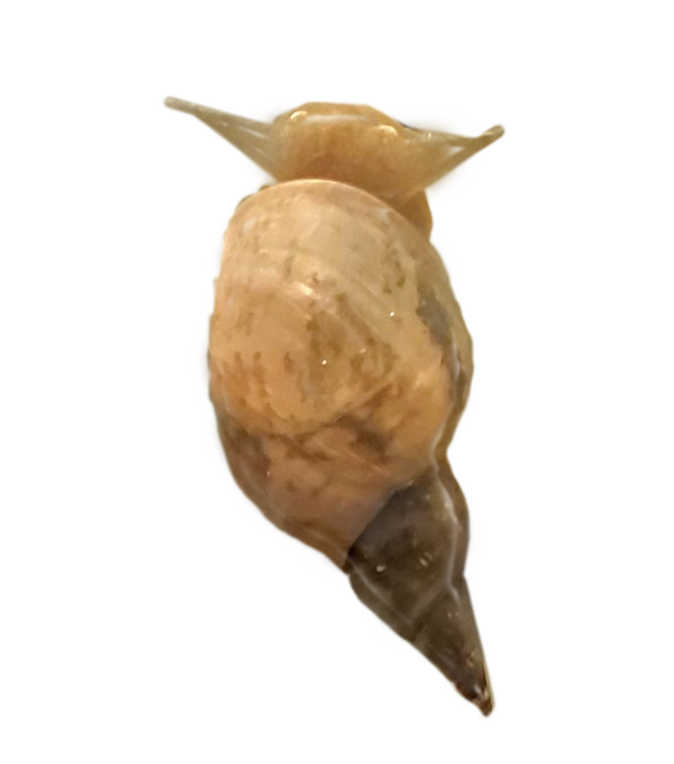
\includegraphics[width=\linewidth]{intro/lymnaea.png}
			
			\column{0.6\textwidth}
			\vspace{-4cm} % Adjust this value to align the text as needed
			\begin{itemize}
				\item<1->In this thesis we work with the neural system of \textit{Lymnaea stagnalis}.
				\item<2>A pond snail whose system is well studied and described.
			\end{itemize}
		\end{columns}
	
\end{frame}

\begin{frame}{Neural stimulation}
	\only<1-3>{
	When studying neural systems, we need neuromodulatory techniques.
	\begin{itemize}
		\item <1-> To study different conditions.
		\item <2-> Test their robustness.
		\item <3-> Simulate external inputs.
	\end{itemize}
	}
	\only<4->{We can classify them based on: 
	\begin{itemize}
		\item<5-> The change in the system: Invasive / \textcolor<13>{red}{non-invasive}
		\item<6-> The source of the stimulation: 
			\begin{itemize}
				\item<7->{Chemical}
				\item<8->\textcolor<12>{red}{Electrical}
				\item<9->{Magnetic}
				\item<10->{Mechanical}
				\item<11->\textcolor<13>{red}{Optical}			
			\end{itemize}
	\end{itemize}	
}
%TODO añadir figuras (mucho texto)
		
\end{frame}

\section{Motivation and Objectives}
\begin{frame}{Motivation and Objectives}
	\begin{enumerate}
		\only<1-6>{
			\item<1-> To explore the \textbf{sequential nature of neuronal dynamics} at distinct description levels.
			\item<2-> To study \textbf{sequence interval variability} constraints and relationships in neural models and living circuits.
			\item<3-> To analyze the feeding CPG of \textit{Lymnaea stagnalis} to provide evidence of the\textbf{ universality of sequential dynamical invariants} found in the pyloric CPG by:
			\begin{enumerate}
				\item<4-> Characterizing the sequential invariants cycle-by-cycle in a bursting CPG model.
				\item<5-> Analyzing intracellular recordings with spontaneous activity and with different rhythm initiation stimulation protocols.
			\end{enumerate}
			\item<6-> To illustrate the possible \textbf{functionality} of sequential dynamical invariants in biohybrid robotics.
		}
		\only<7-11>{
			\setcounter{enumi}{4}
			\item<7-> To test the capability of \textbf{CW-NIR laser stimulation to modulate} neuronal dynamics by:
			\begin{enumerate}
				\item<8-> Characterizing the CW-NIR effect in the spike waveform dynamics.
				\item<9-> Analyzing the ability of this neurotechnology to change the spiking rate and the circuit dynamics.
			\end{enumerate}
			\item<10-> To study the possible \textbf{biophysical candidates} underlying the CW-NIR effect in model simulations.
			\item<11-> To design and implement a \textbf{new technique} for CW-NIR stimulation in \textbf{closed-loop}.
		}
	\end{enumerate}
	
\end{frame}


\section[Sequential Dynamical Invariants]{Sequential constrains in CPG circuits:
	Dynamical invariants}

\begin{frame}{Central Pattern Generators}
	\only<1-4>{
		\begin{itemize}
			\item<1->{Neural circuits generating robust sequences of neural activity}
			\item<2->{Control motor rhythms in an autonomous manner}
			\item<3->{Present in vertebrates and invertebrates}
			\item<4->{Flexible enough to adapt the rhythm to the variability keeping a robust sequential activity\\}
		\end{itemize}
%	\\
		\vspace{10pt}
		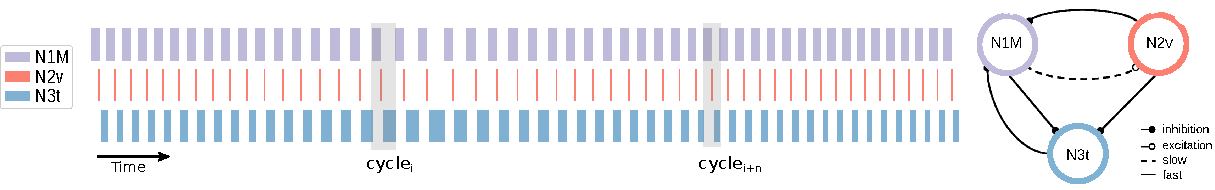
\includegraphics[width=\textwidth]{invariants/variability/sequences_in_cpgs.pdf}
	}
\end{frame}

\begin{frame}{Central Pattern Generators}
		\begin{columns}
			% First column in the first row
			\begin{column}{0.75\textwidth}
				\begin{itemize}
					\item{Non-open topologies}
					\item{Based on mutual inhibition}
					\item{Temporal sequences maintained cycle-by-cycle}
				\end{itemize}
			\end{column}
			% Second column in the first row
			\begin{column}{0.3\textwidth}
				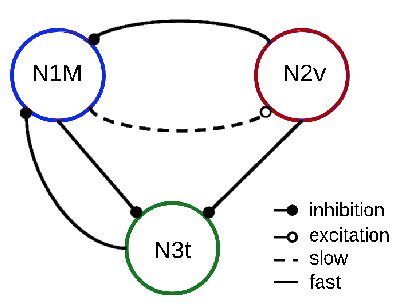
\includegraphics[width=\textwidth]{Images/CPG-topology.png} % Replace 'example-image' with your image file
			\end{column}
		\end{columns}
		
		% Second row
		\begin{figure}[h!]
			\centering
			\movie[label=CPG activity,width=0.7\textwidth,poster=false,autostart=true,showcontrols,loop] 
			{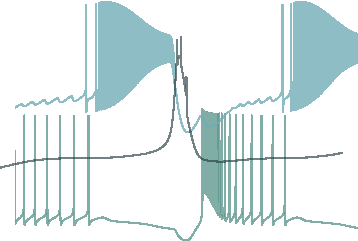
\includegraphics[width=0.7\textwidth]{intro/CPG.pdf}}{Movies/CPG_activity_slow.mp4}
		\end{figure}	
	%TODO arreglar tamaño video	
\end{frame}

\begin{frame}{Temporal constrains: Sequential Dynamical invariants}

		\begin{itemize}
			\item<1->Recently found in pyloric CPG (experimental study). (Elices et al.)
			\item<1->Specific intervals that build the sequence are highly correlated cycle-by-cycle.
			\item<1->Consistent under high variability induced situations (Ethanol).
		\end{itemize}
	\begin{figure}[h!]
		\centering
		\movie[label=pyloric video,width=\textwidth,poster=false,autostart=true,start=120s,showcontrols,loop]
		{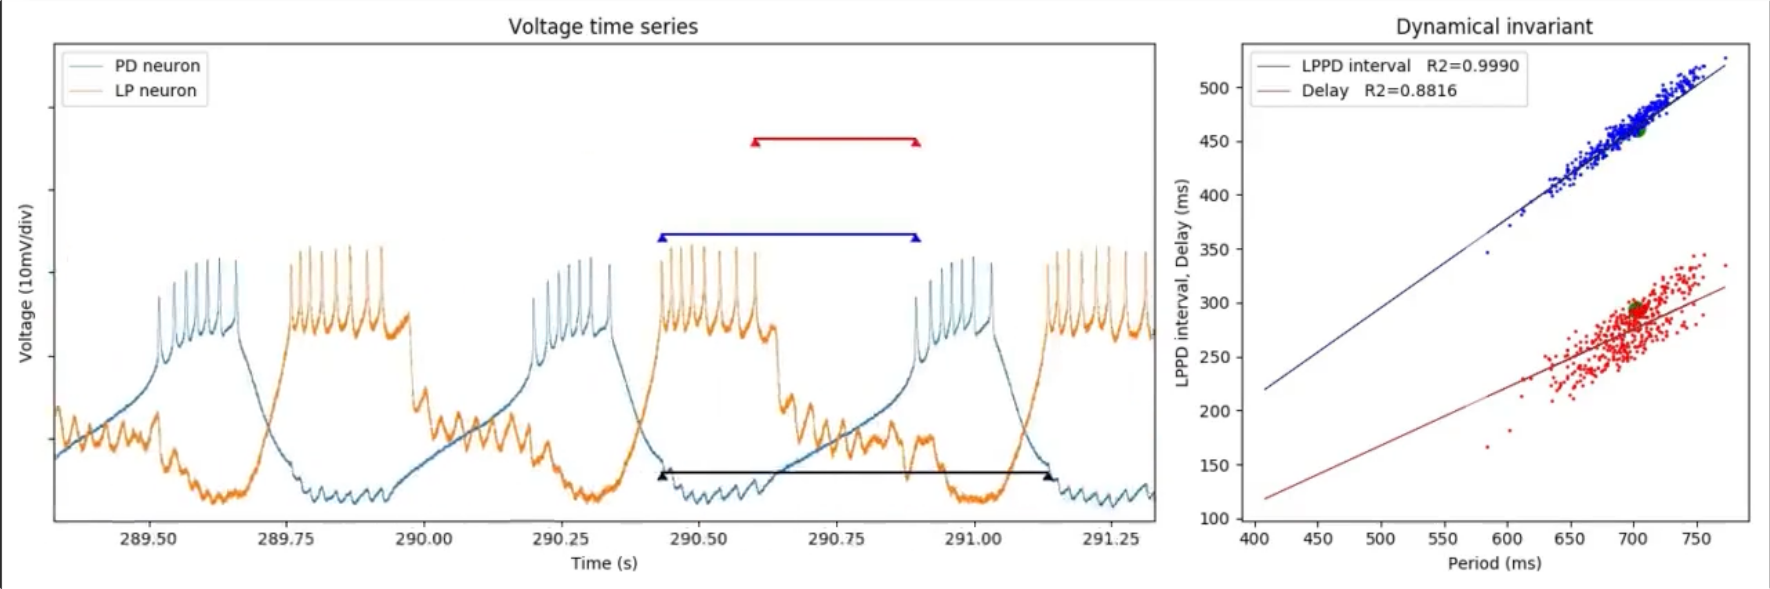
\includegraphics[width=\textwidth]{Movies/elices_invariants.png}}{Movies/elices_invariants.mp4}
	\end{figure}
%TODO arreglar tamaño video
\end{frame}

\begin{frame}{Feeding CPG of \textit{Lymnaea stagnalis}}

	Triphasic rhythm:
	\\
	\centering
	N1 phase $\rightarrow$ N2 phase $\rightarrow$ N3 phase \\
	Protraction $\rightarrow$ Rasp $\rightarrow$ Swallow\\
	\vspace{3pt}
	
	\movie[label=cpg video,width=\textwidth,autostart,loop] 
	{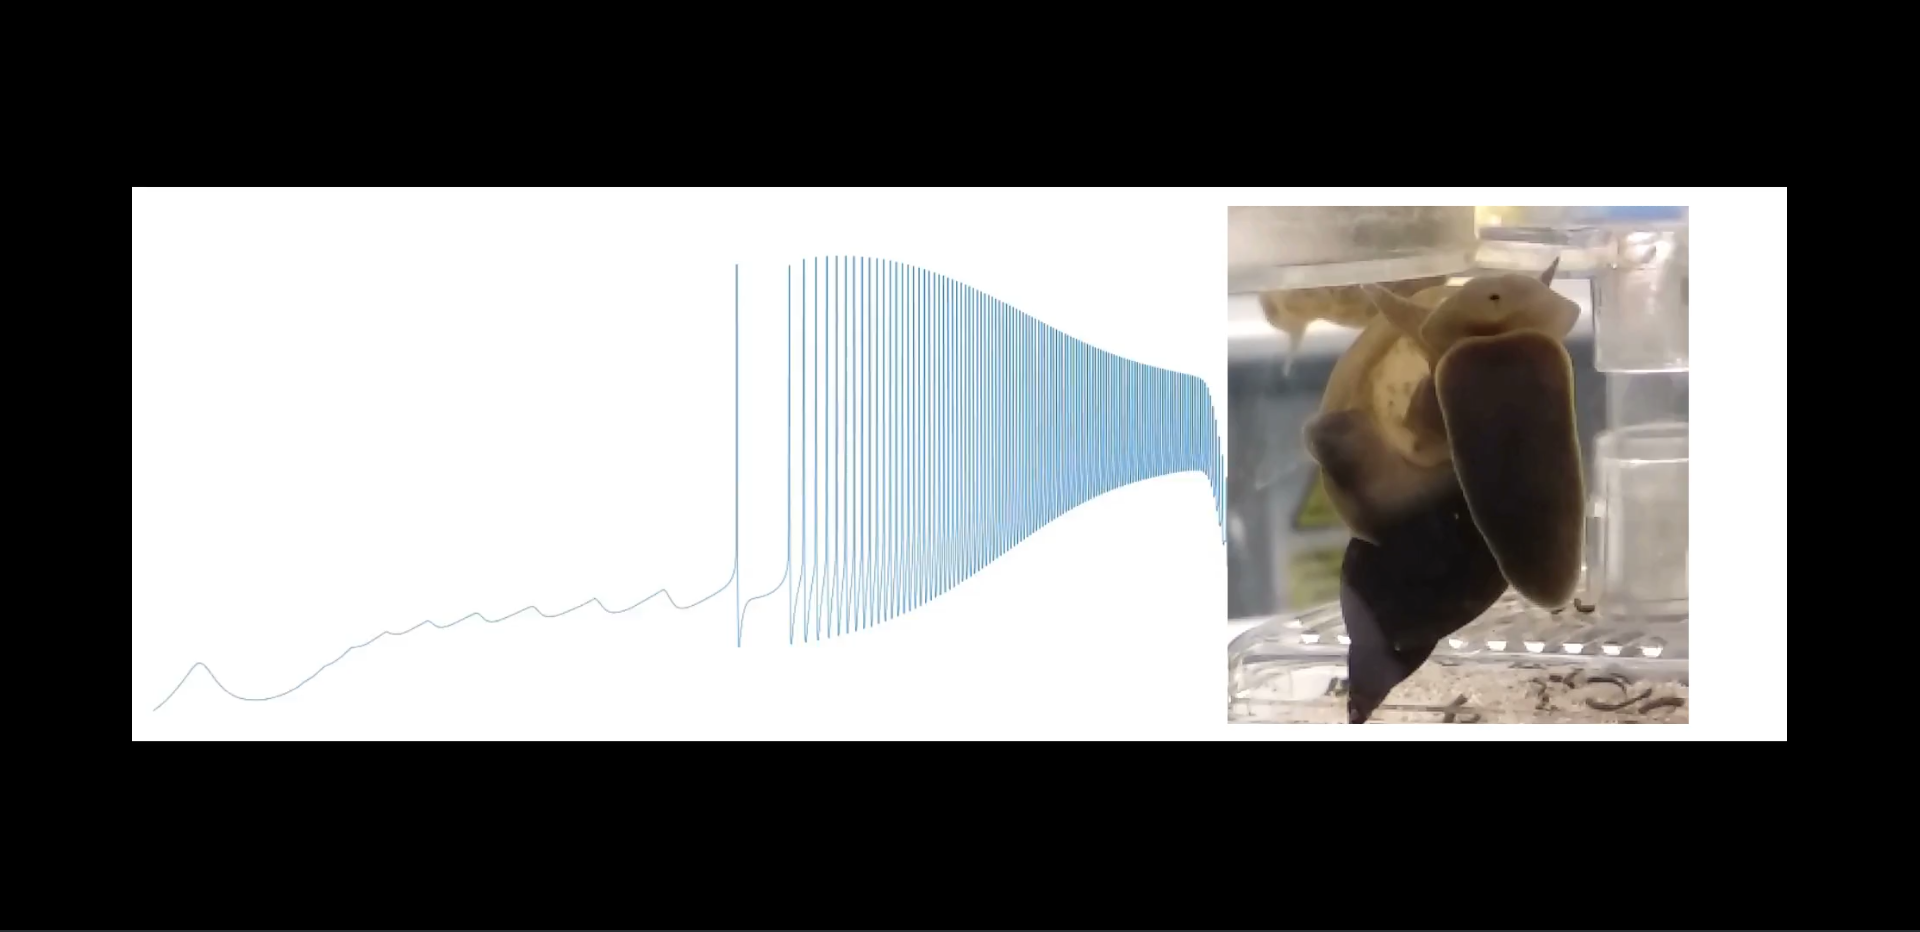
\includegraphics[width=\textwidth]{Images/CPG-lymnaea_v2_mejorado.png}}{Movies/CPG-lymnaea_v2_mejorado.mp4}

%	\begin{itemize}
%		\item<1->{N1 phase $\rightarrow$ Protraction}
%		\item<1->{N2 phase $\rightarrow$ Rasp}
%		\item<1->{N3 phase $\rightarrow$ Swallow}
%	\end{itemize}

	%TODO Video pantalla completa y señalar a la boca
\end{frame}



\begin{frame}{Computational and Experimental approach}
	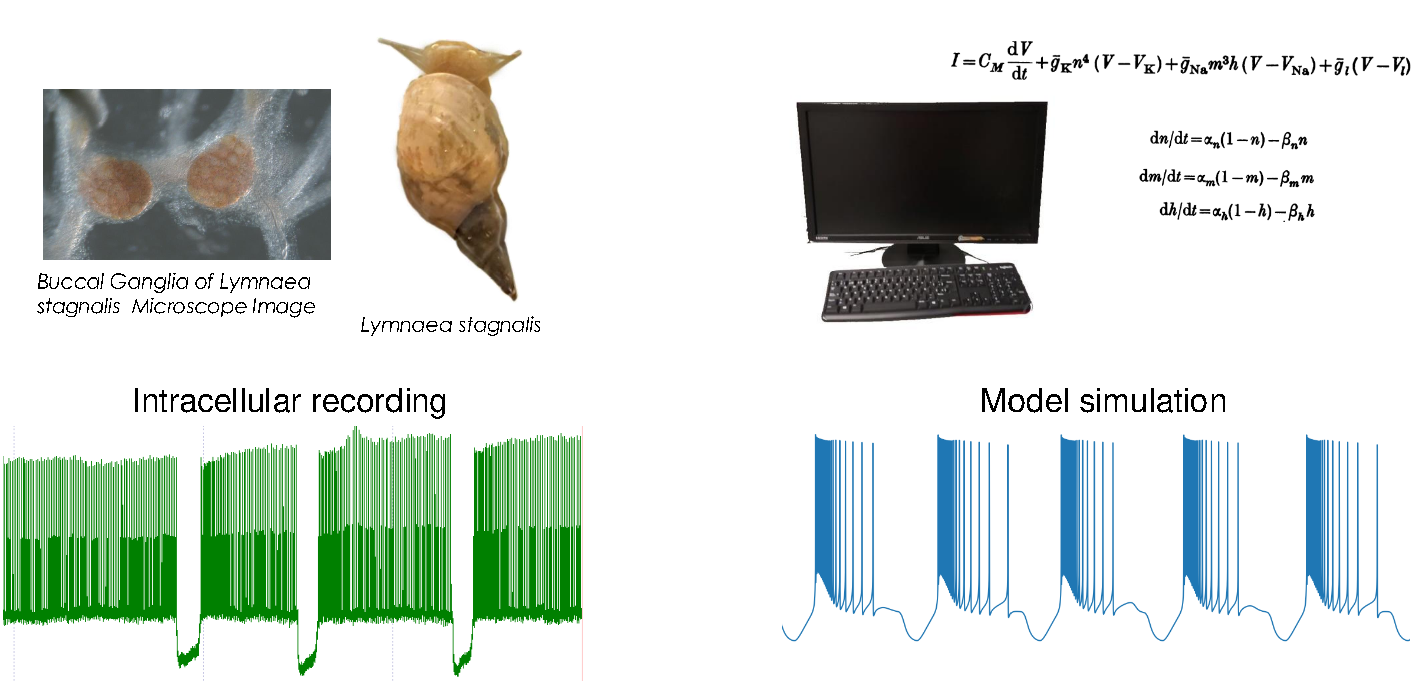
\includegraphics[width=\textwidth]{Images/experimental-computational.pdf})
	\note{DECIR "experimental TECHNIQUES"}
\end{frame}




\begin{frame}{Characterization of the time-intervals cycle-by-cycle}
	\only<2-3>{
	To analyze the dynamics of the sequential activity cycle-by-cycle we need to define time references to characterize the time-intervals in the sequence.
	\vspace{5pt}
	\begin{columns}
		\uncover<2->{
		\begin{column}{0.4\textwidth}
			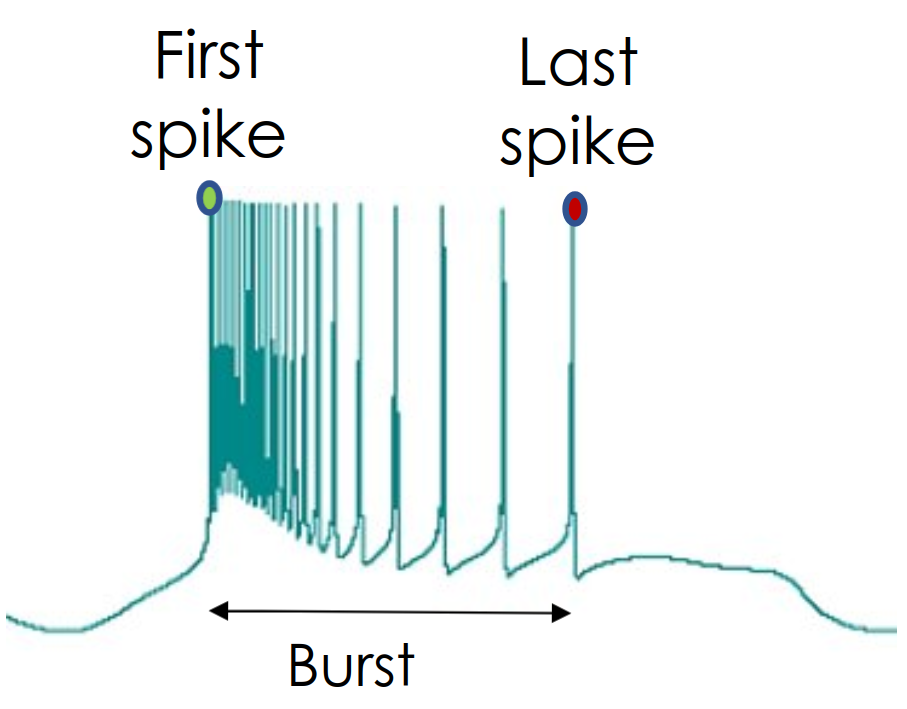
\includegraphics[width=\textwidth]{Images/time-references.png}
		\end{column}
	}
	\uncover<3->{
		\begin{column}{0.6\textwidth}
			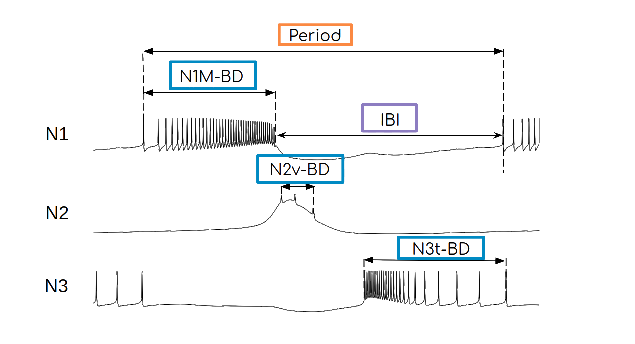
\includegraphics[width=\textwidth]{methods-paper-modelo/figure4a.eps}
		\end{column}
	}
	\end{columns}
	}
	\uncover<4->{We can also define intervals combining the time references of two bursts}
	\only<4>{
		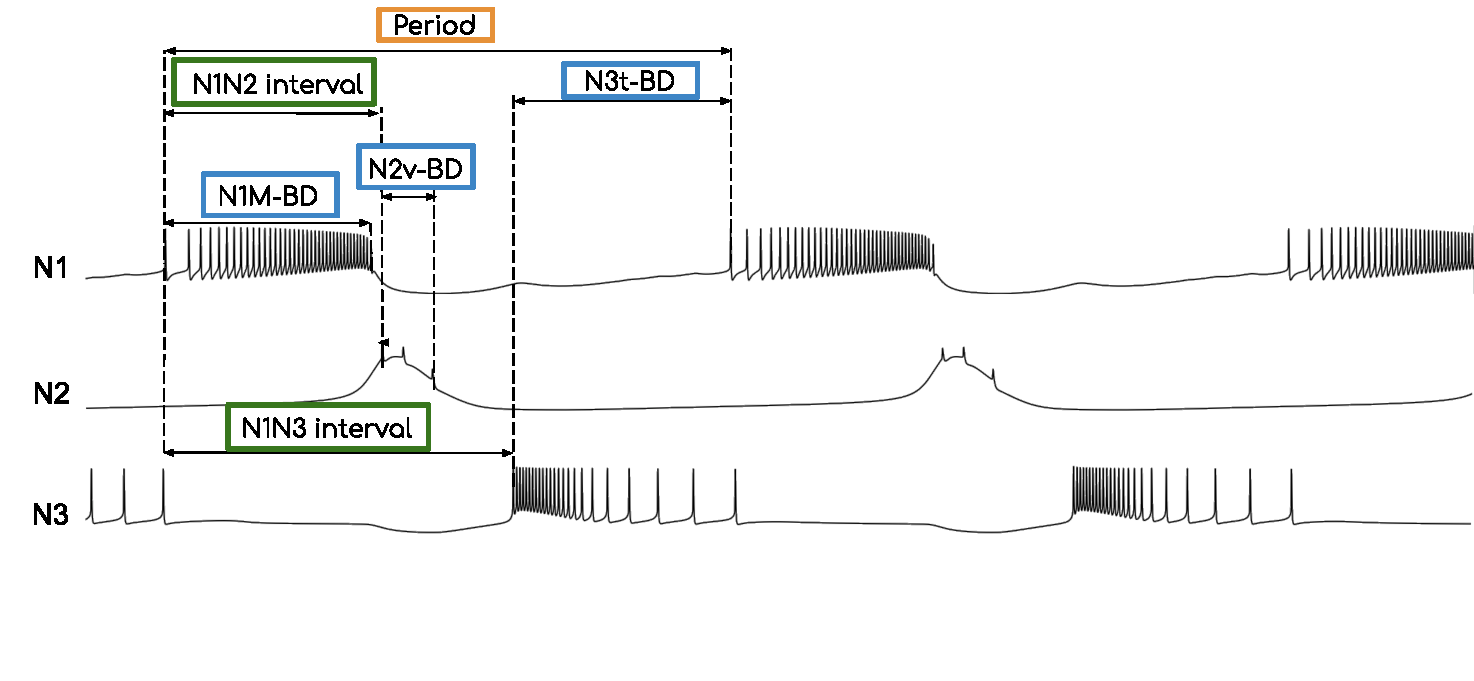
\includegraphics[width=\textwidth]{Images/Intervals_figure_complete_only_intervals_n1.pdf}
	}

	\only<5>{
		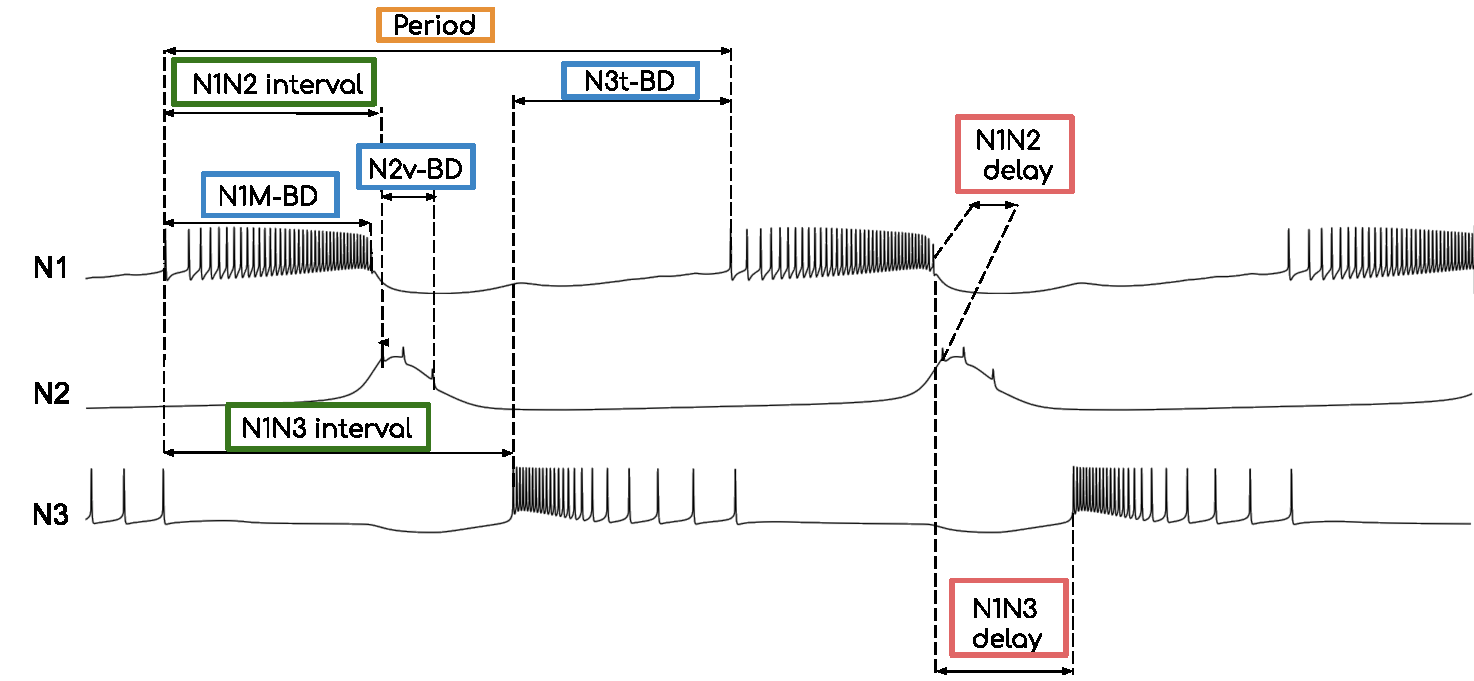
\includegraphics[width=\textwidth]{Images/Intervals_figure_complete_only_intervals_n1-delay.pdf}
	}
	\only<6>{
	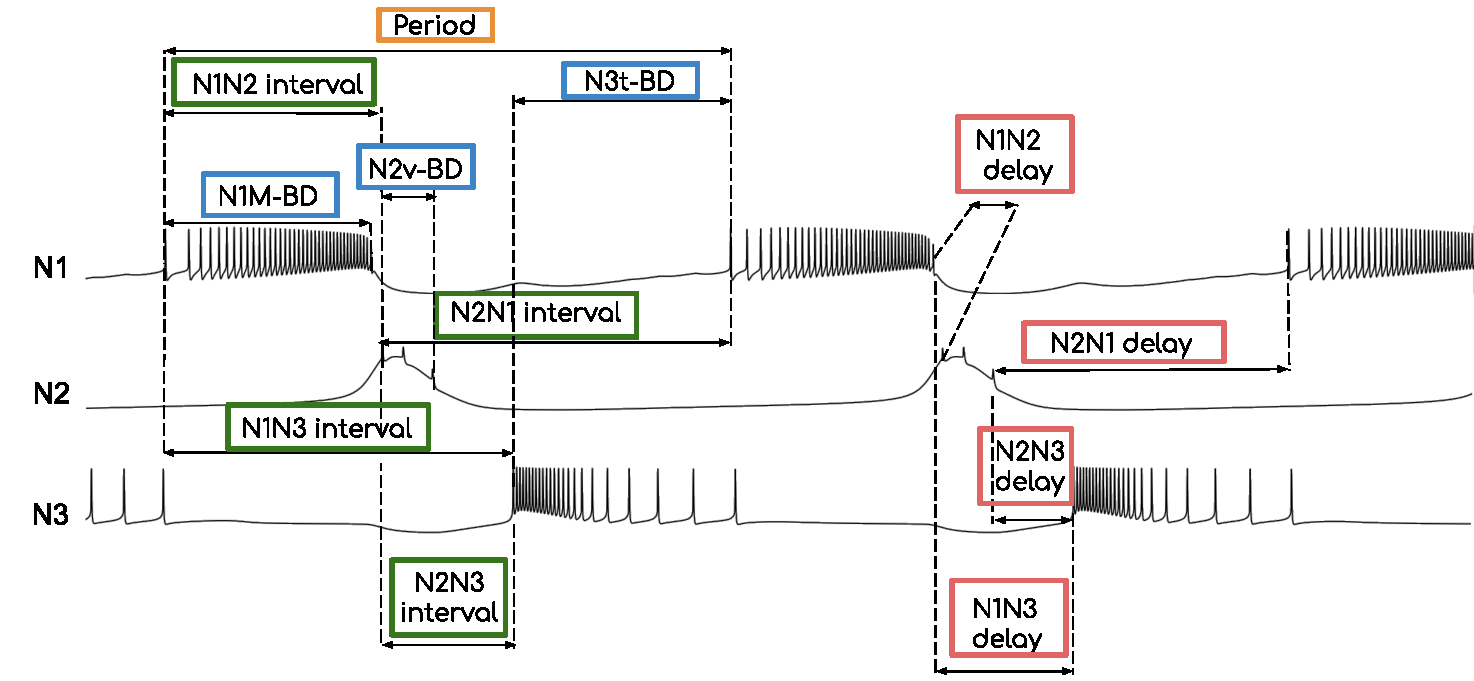
\includegraphics[width=\textwidth]{Images/Intervals_figure_complete_only_intervals_n2.pdf}
	}	
	\only<7>{
		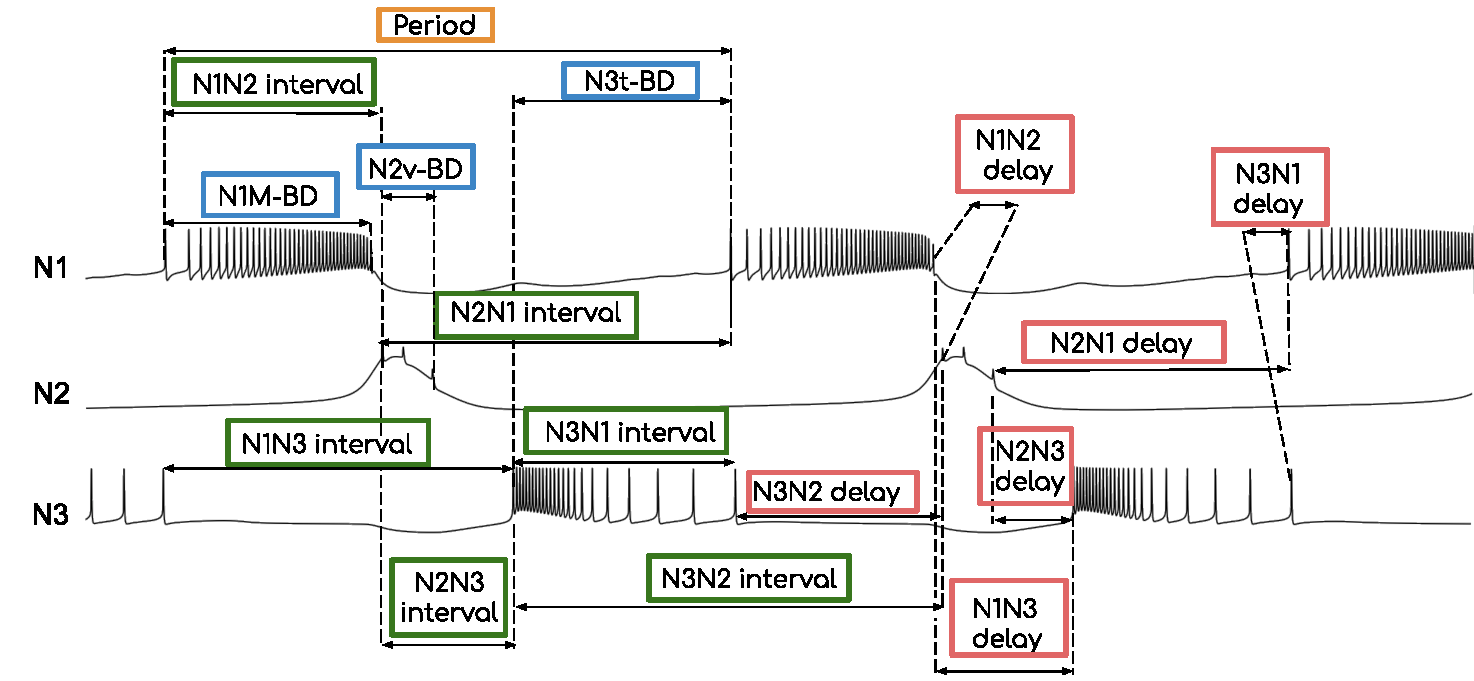
\includegraphics[width=\textwidth]{Images/Intervals_figure_complete_only_intervals_n3.pdf}
	}

	

\end{frame}


\begin{frame}{Computational Approach: Model description}
	\begin{columns}
		\begin{column}{0.5\textwidth}
			\begin{itemize}
				\item<1->(Vavoulis et al.)
				\item<1->Conductance-based model.
				\item<1->Specific waveforms and gradual synapse.
				\item<1->Two compartments.
				\item<1->Feeding CPG Model.
			\end{itemize}
		\end{column}
		\begin{column}{0.5\textwidth}
			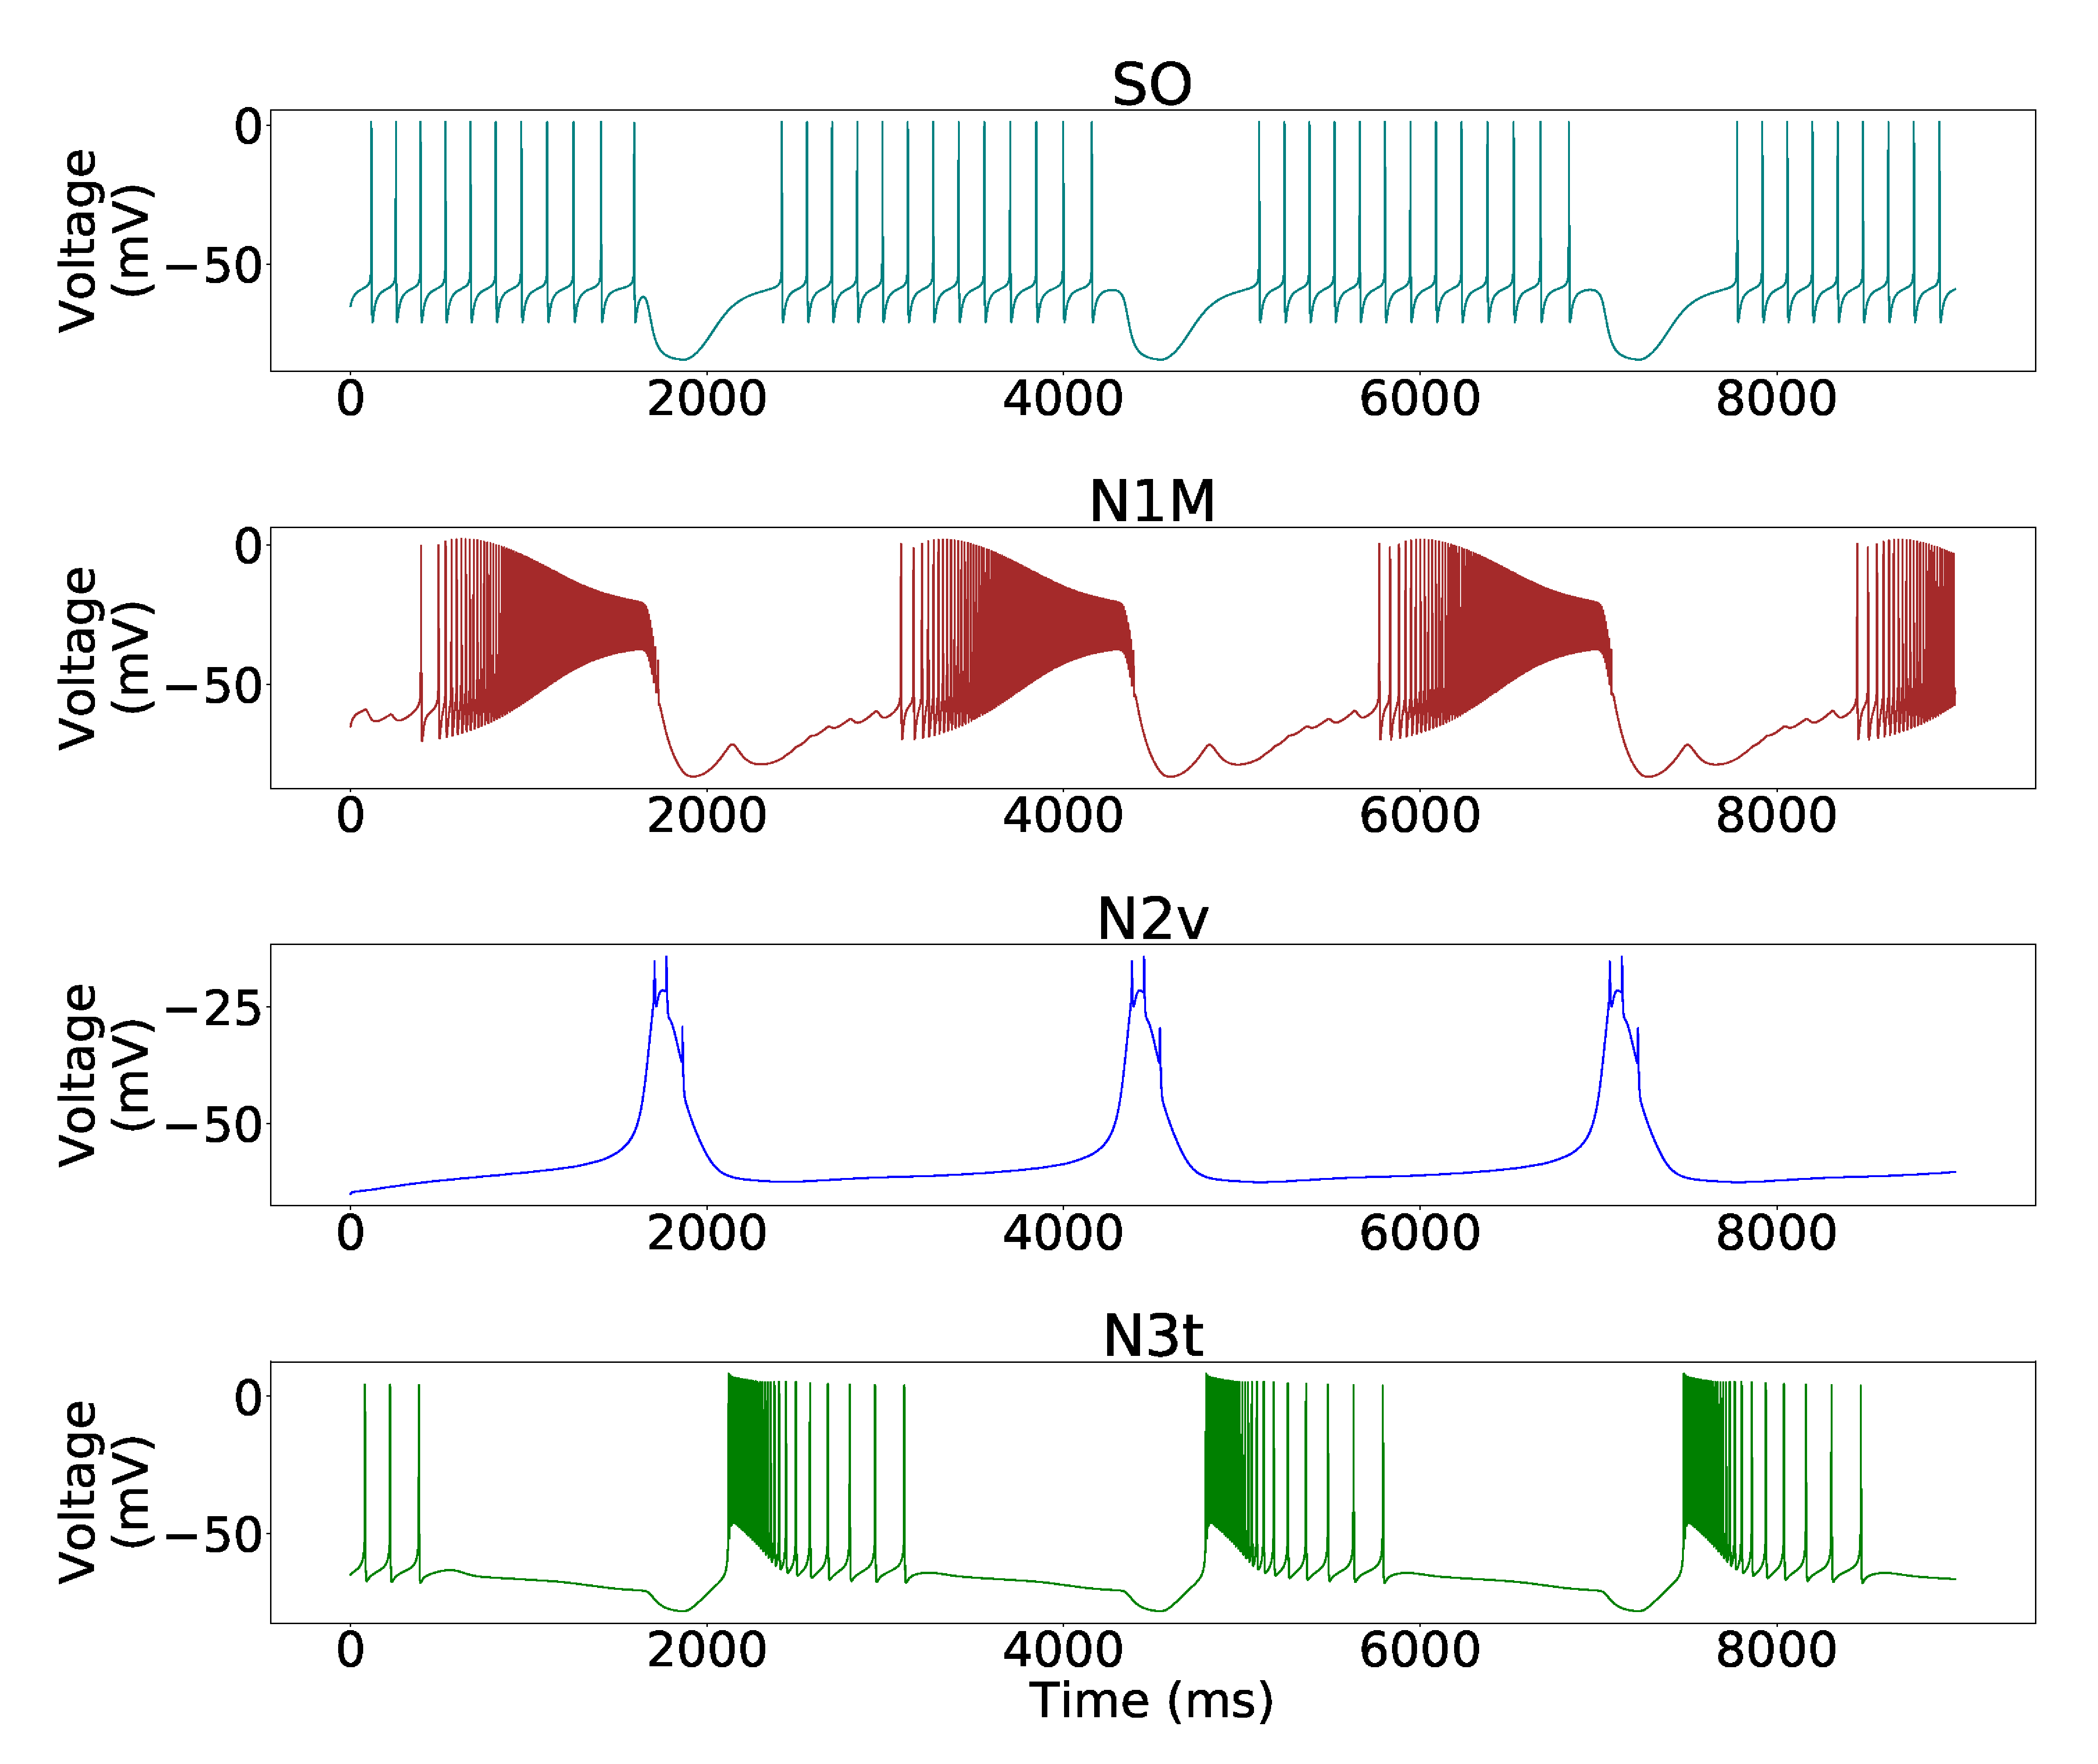
\includegraphics[width=\textwidth]{methods/invariants-model/figure2.eps}
		\end{column}
	\end{columns}
		\vspace{4pt}
		\centering
		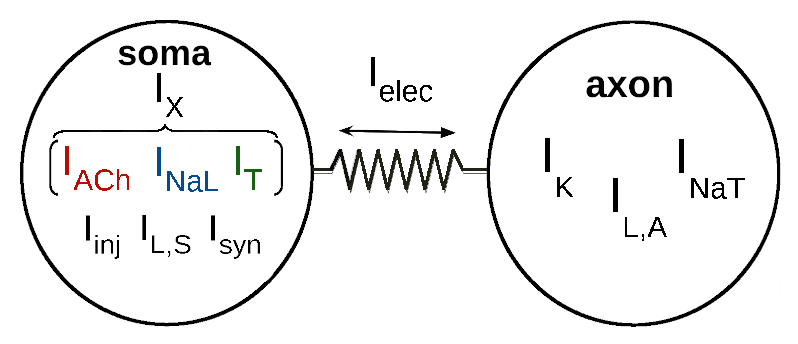
\includegraphics[width=0.6\textwidth]{methods/invariants-model/figure1a.eps}
\end{frame}



\begin{frame}{Computational Approach: Ramp stimulation protocol}
	\centering
	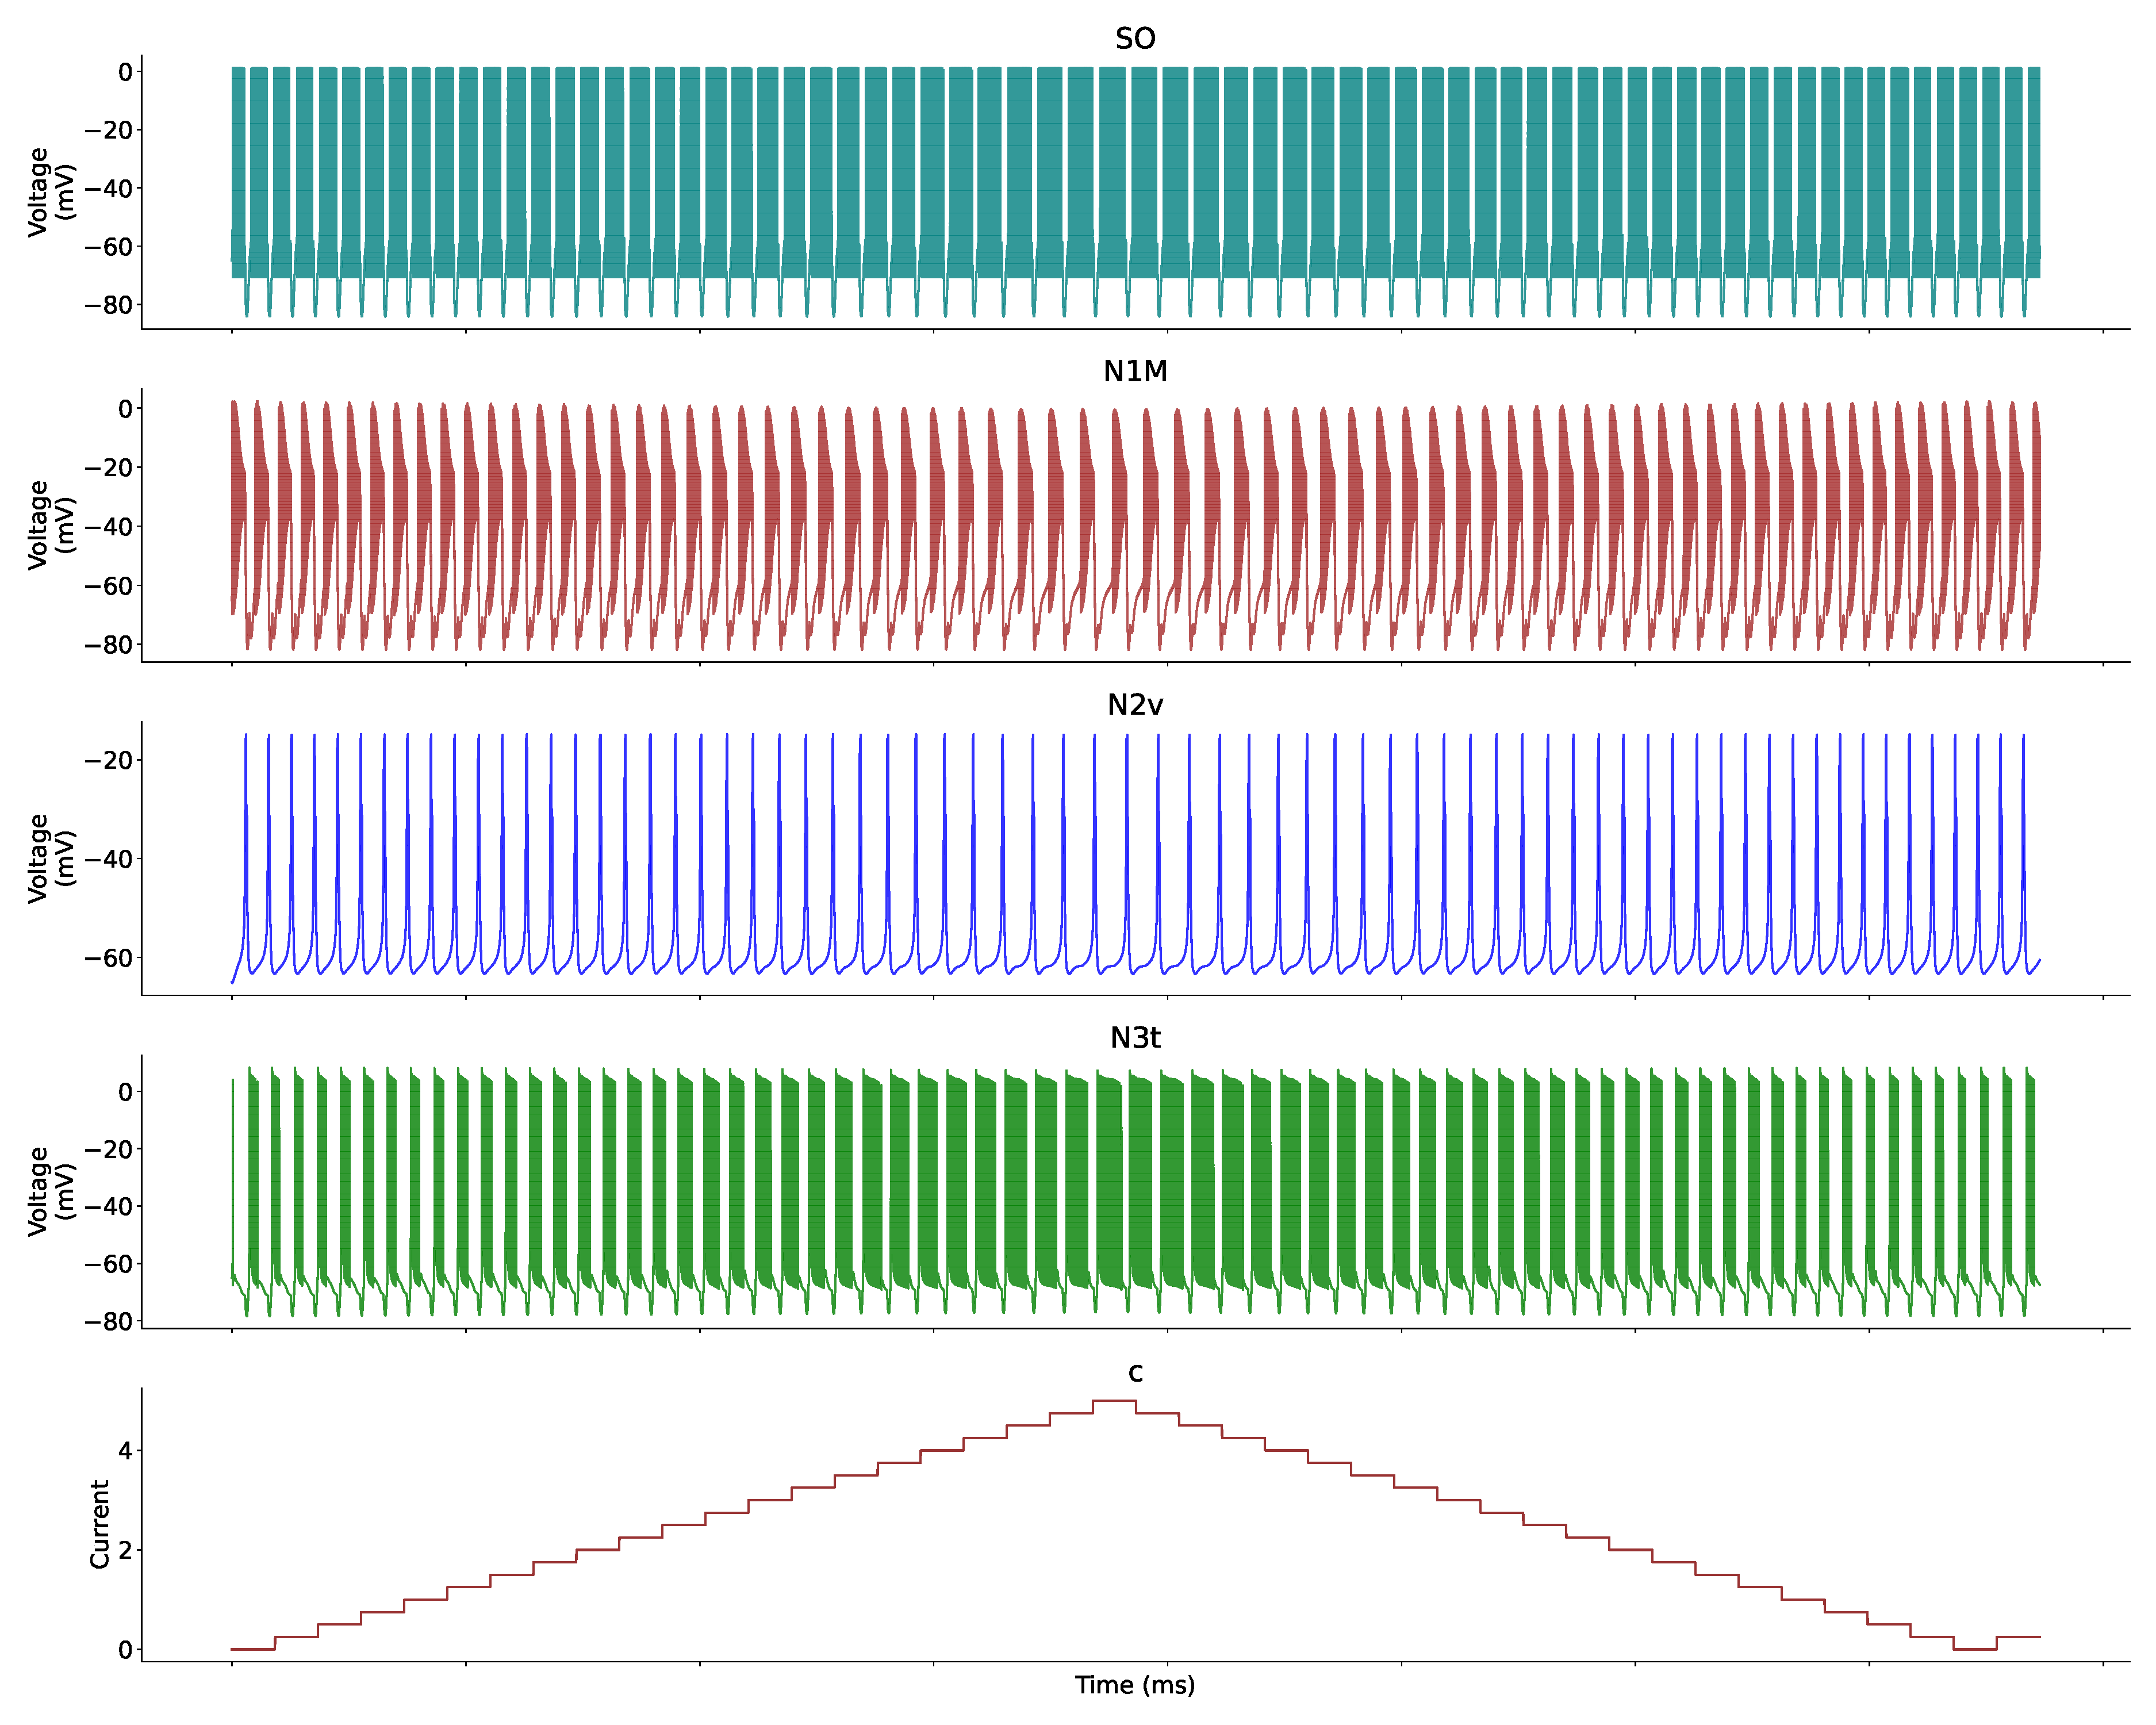
\includegraphics[width=0.8\textwidth]{methods-paper-modelo/circuit_w_current.pdf}
\end{frame}

\begin{frame}{Cycle-by-cycle restrictions}
	\movie[label=model_invariants_video,width=\textwidth,poster,autostart,borderwidth=-5pt,showcontrols,loop] 
	{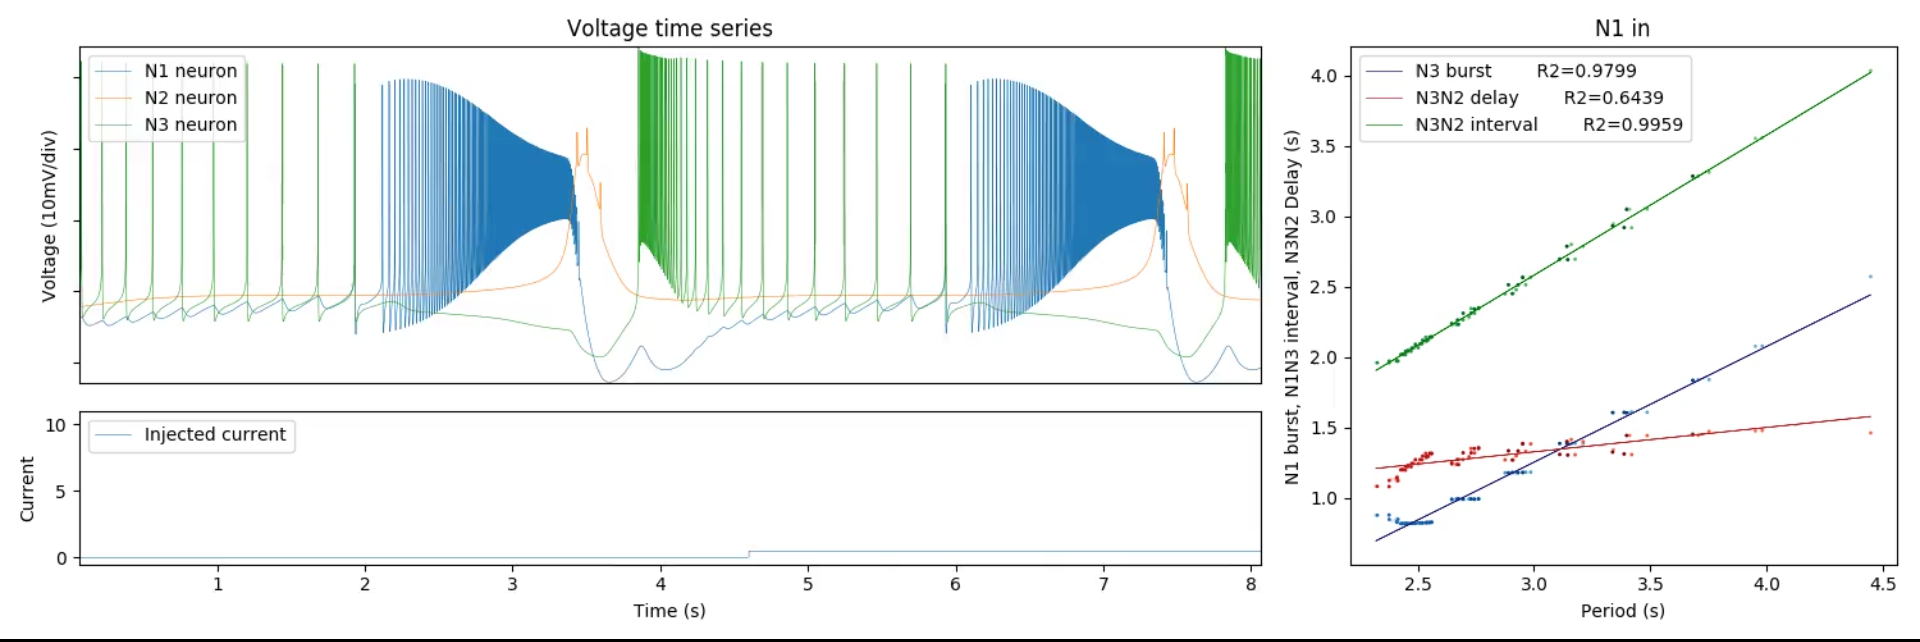
\includegraphics[width=\textwidth]{Movies/n3_n2_no_invariant.png}}{Movies/n3_n2_no_invariant.mp4}
	\note{dejar claro valores del que no varía y qué intervalo no está relacionado.}
\end{frame}

\begin{frame}{N1M stimulation}
	\begin{figure}[hbt!]
		\begin{minipage}[b]{0.36\textwidth}
			\centering
			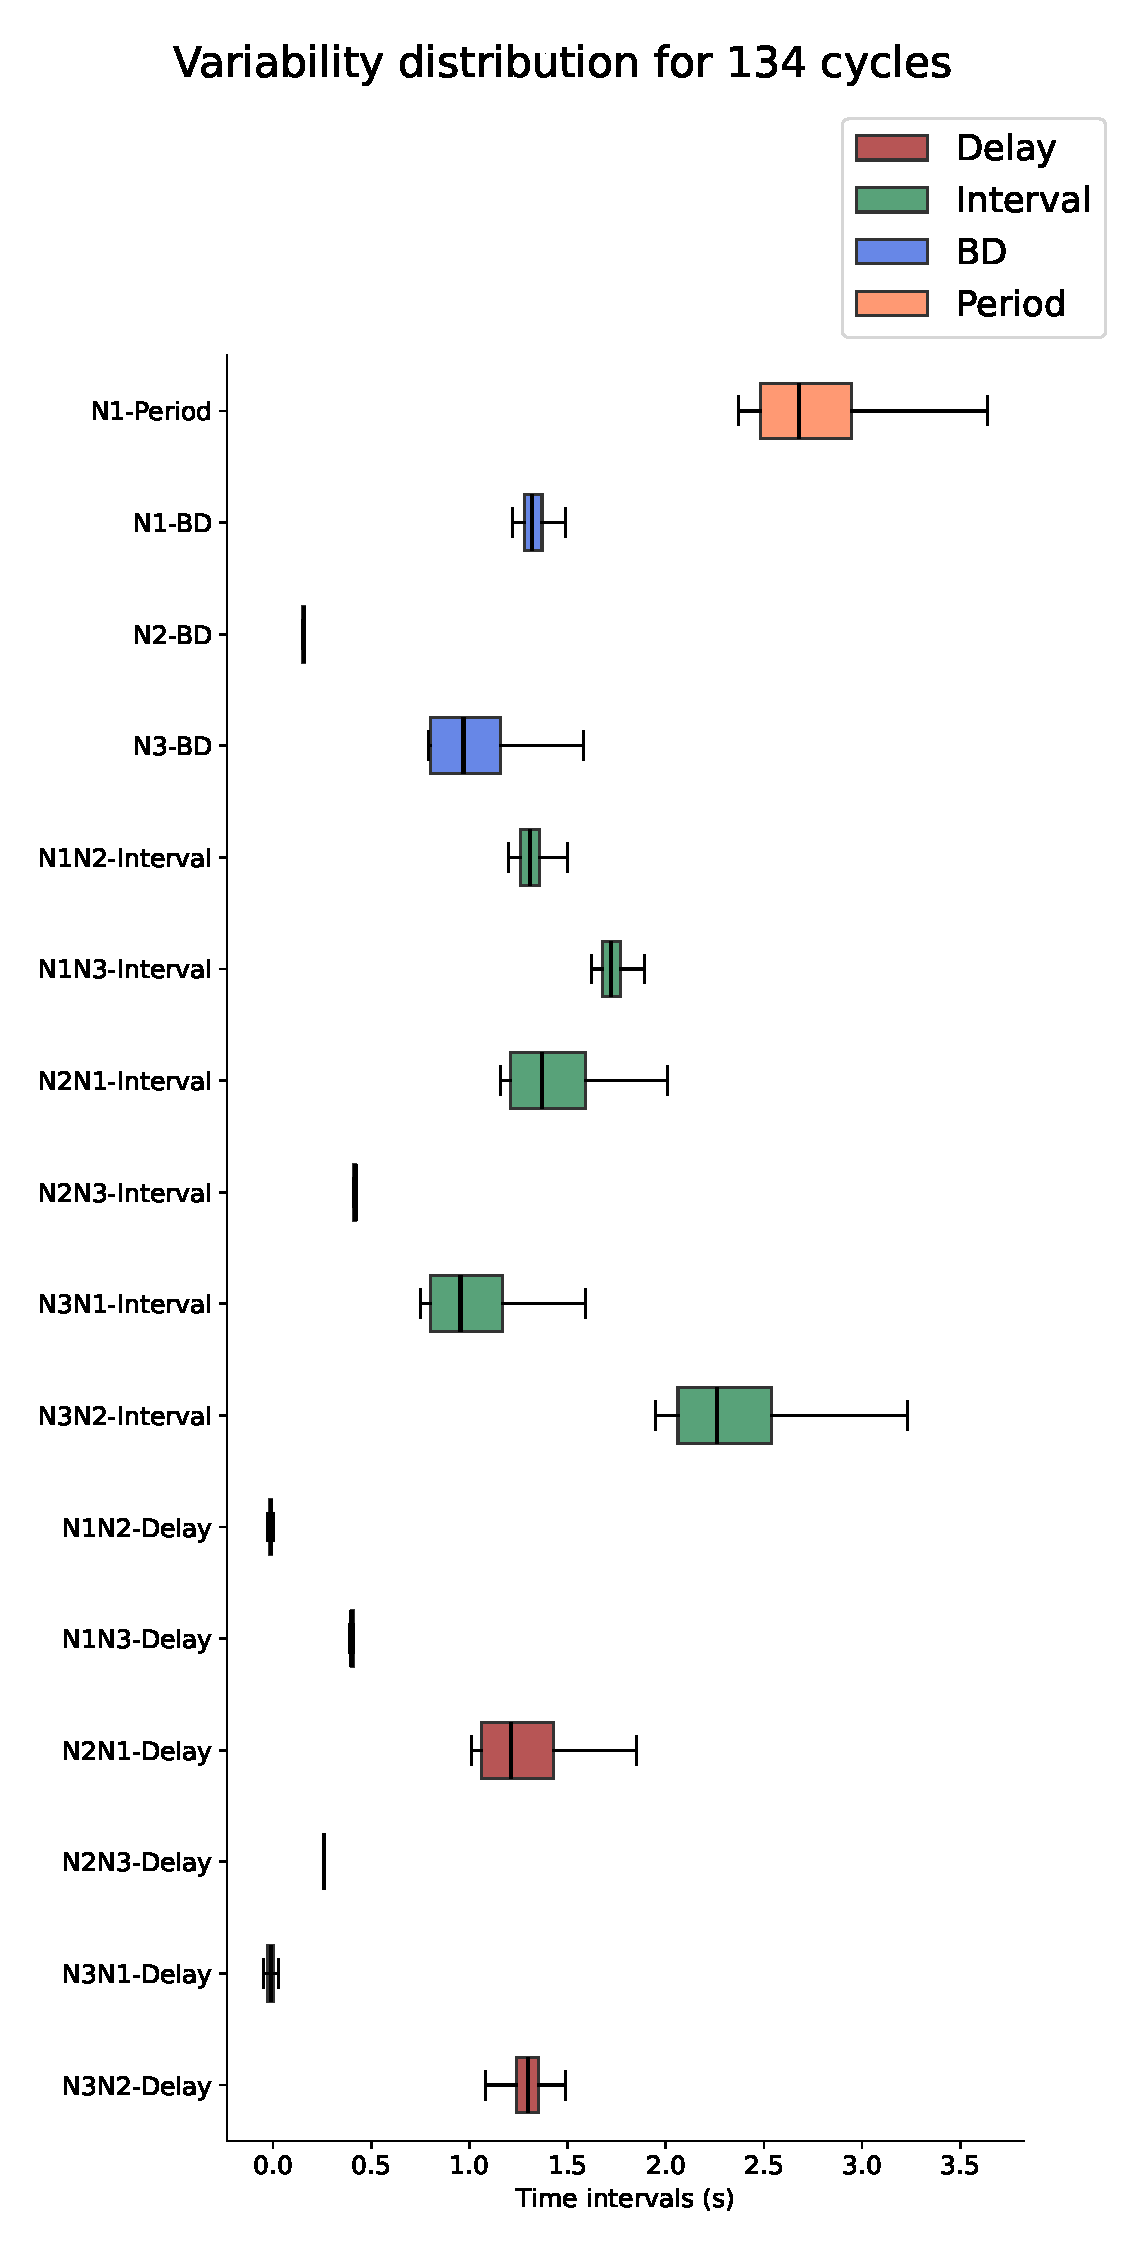
\includegraphics[width=\textwidth]{invariants/data/MODEL/n1m_driven/images/3phases/_boxplot.pdf}
		\end{minipage}
		\begin{minipage}[b]{0.44\textwidth}
			\centering
			\begin{minipage}[b]{\textwidth}
				\centering
				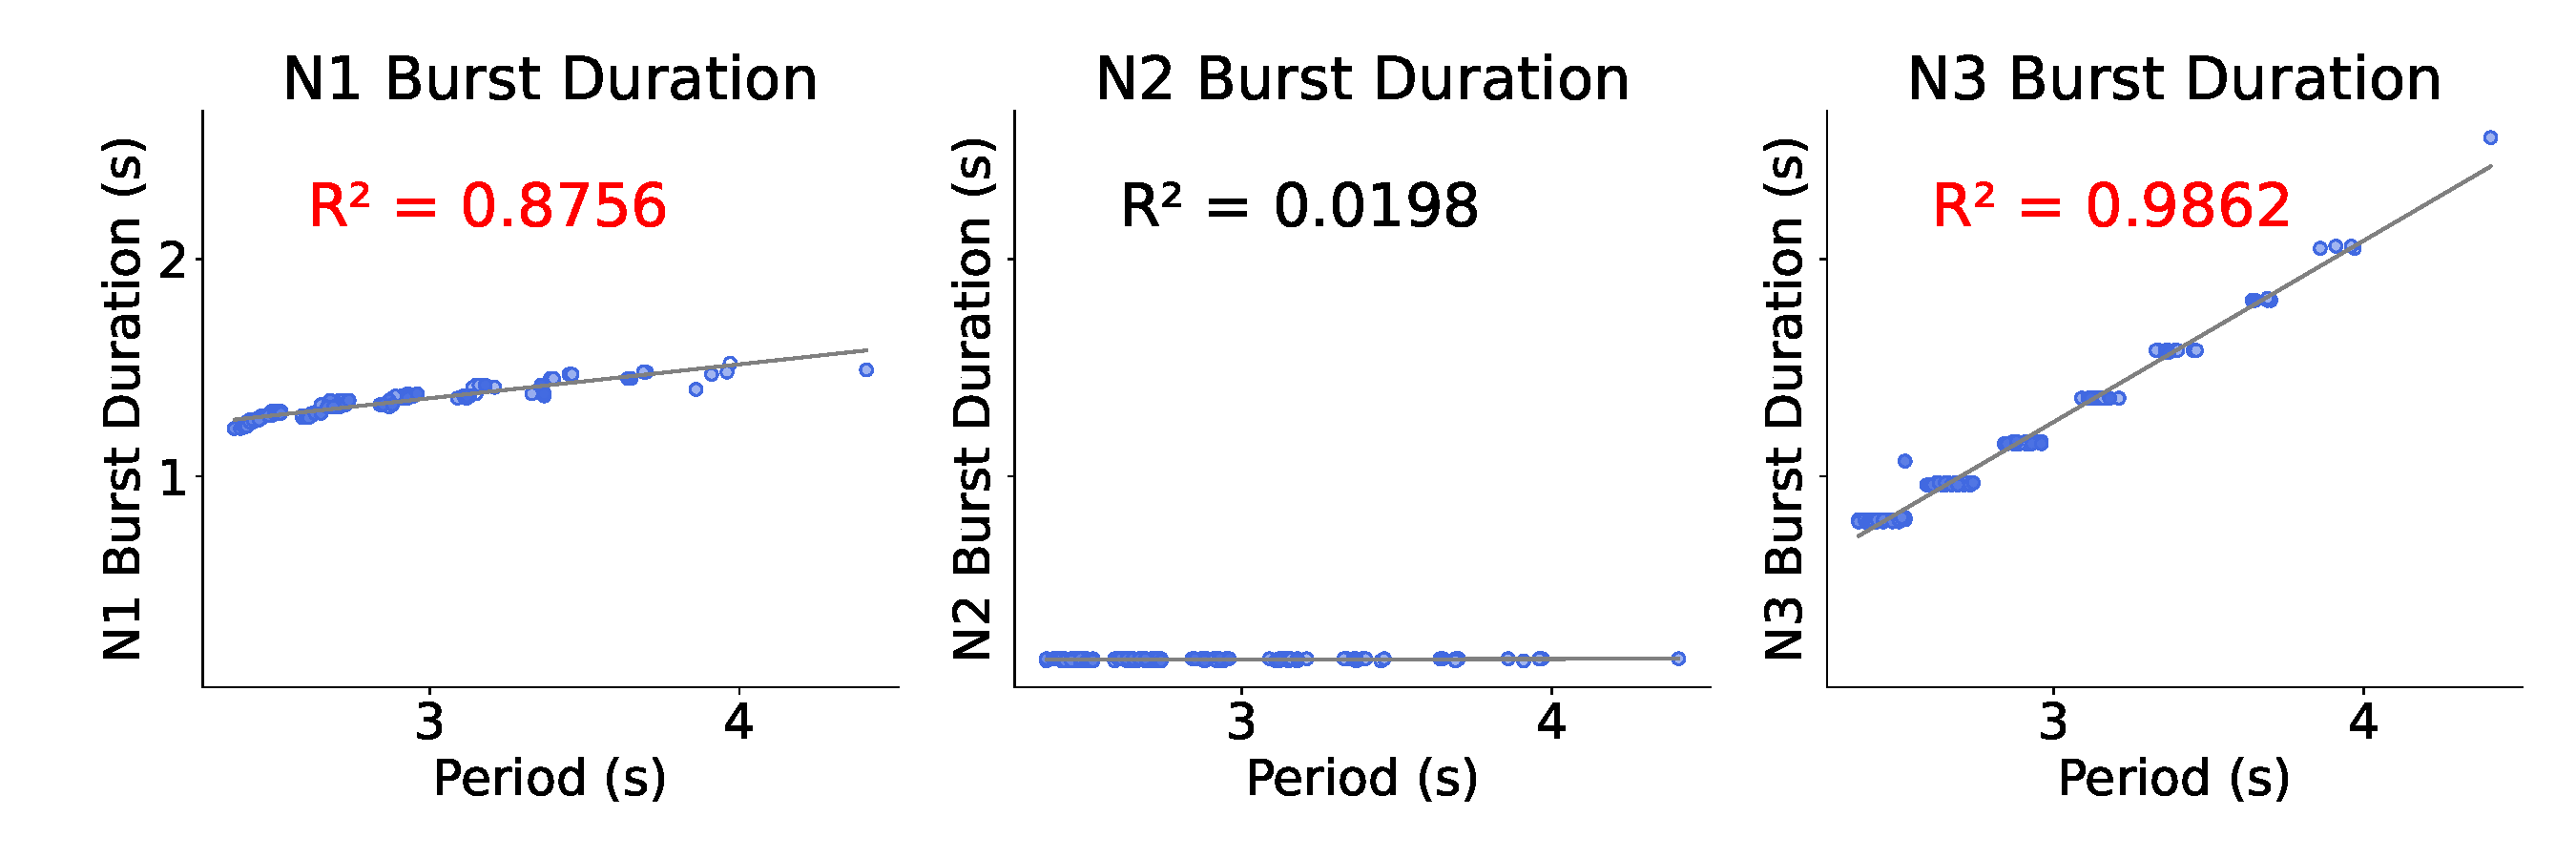
\includegraphics[width=\textwidth]{invariants/data/MODEL/n1m_driven/images/3phases/_durations.pdf}
			\end{minipage}\
			\begin{minipage}[b]{\textwidth}
				\centering
				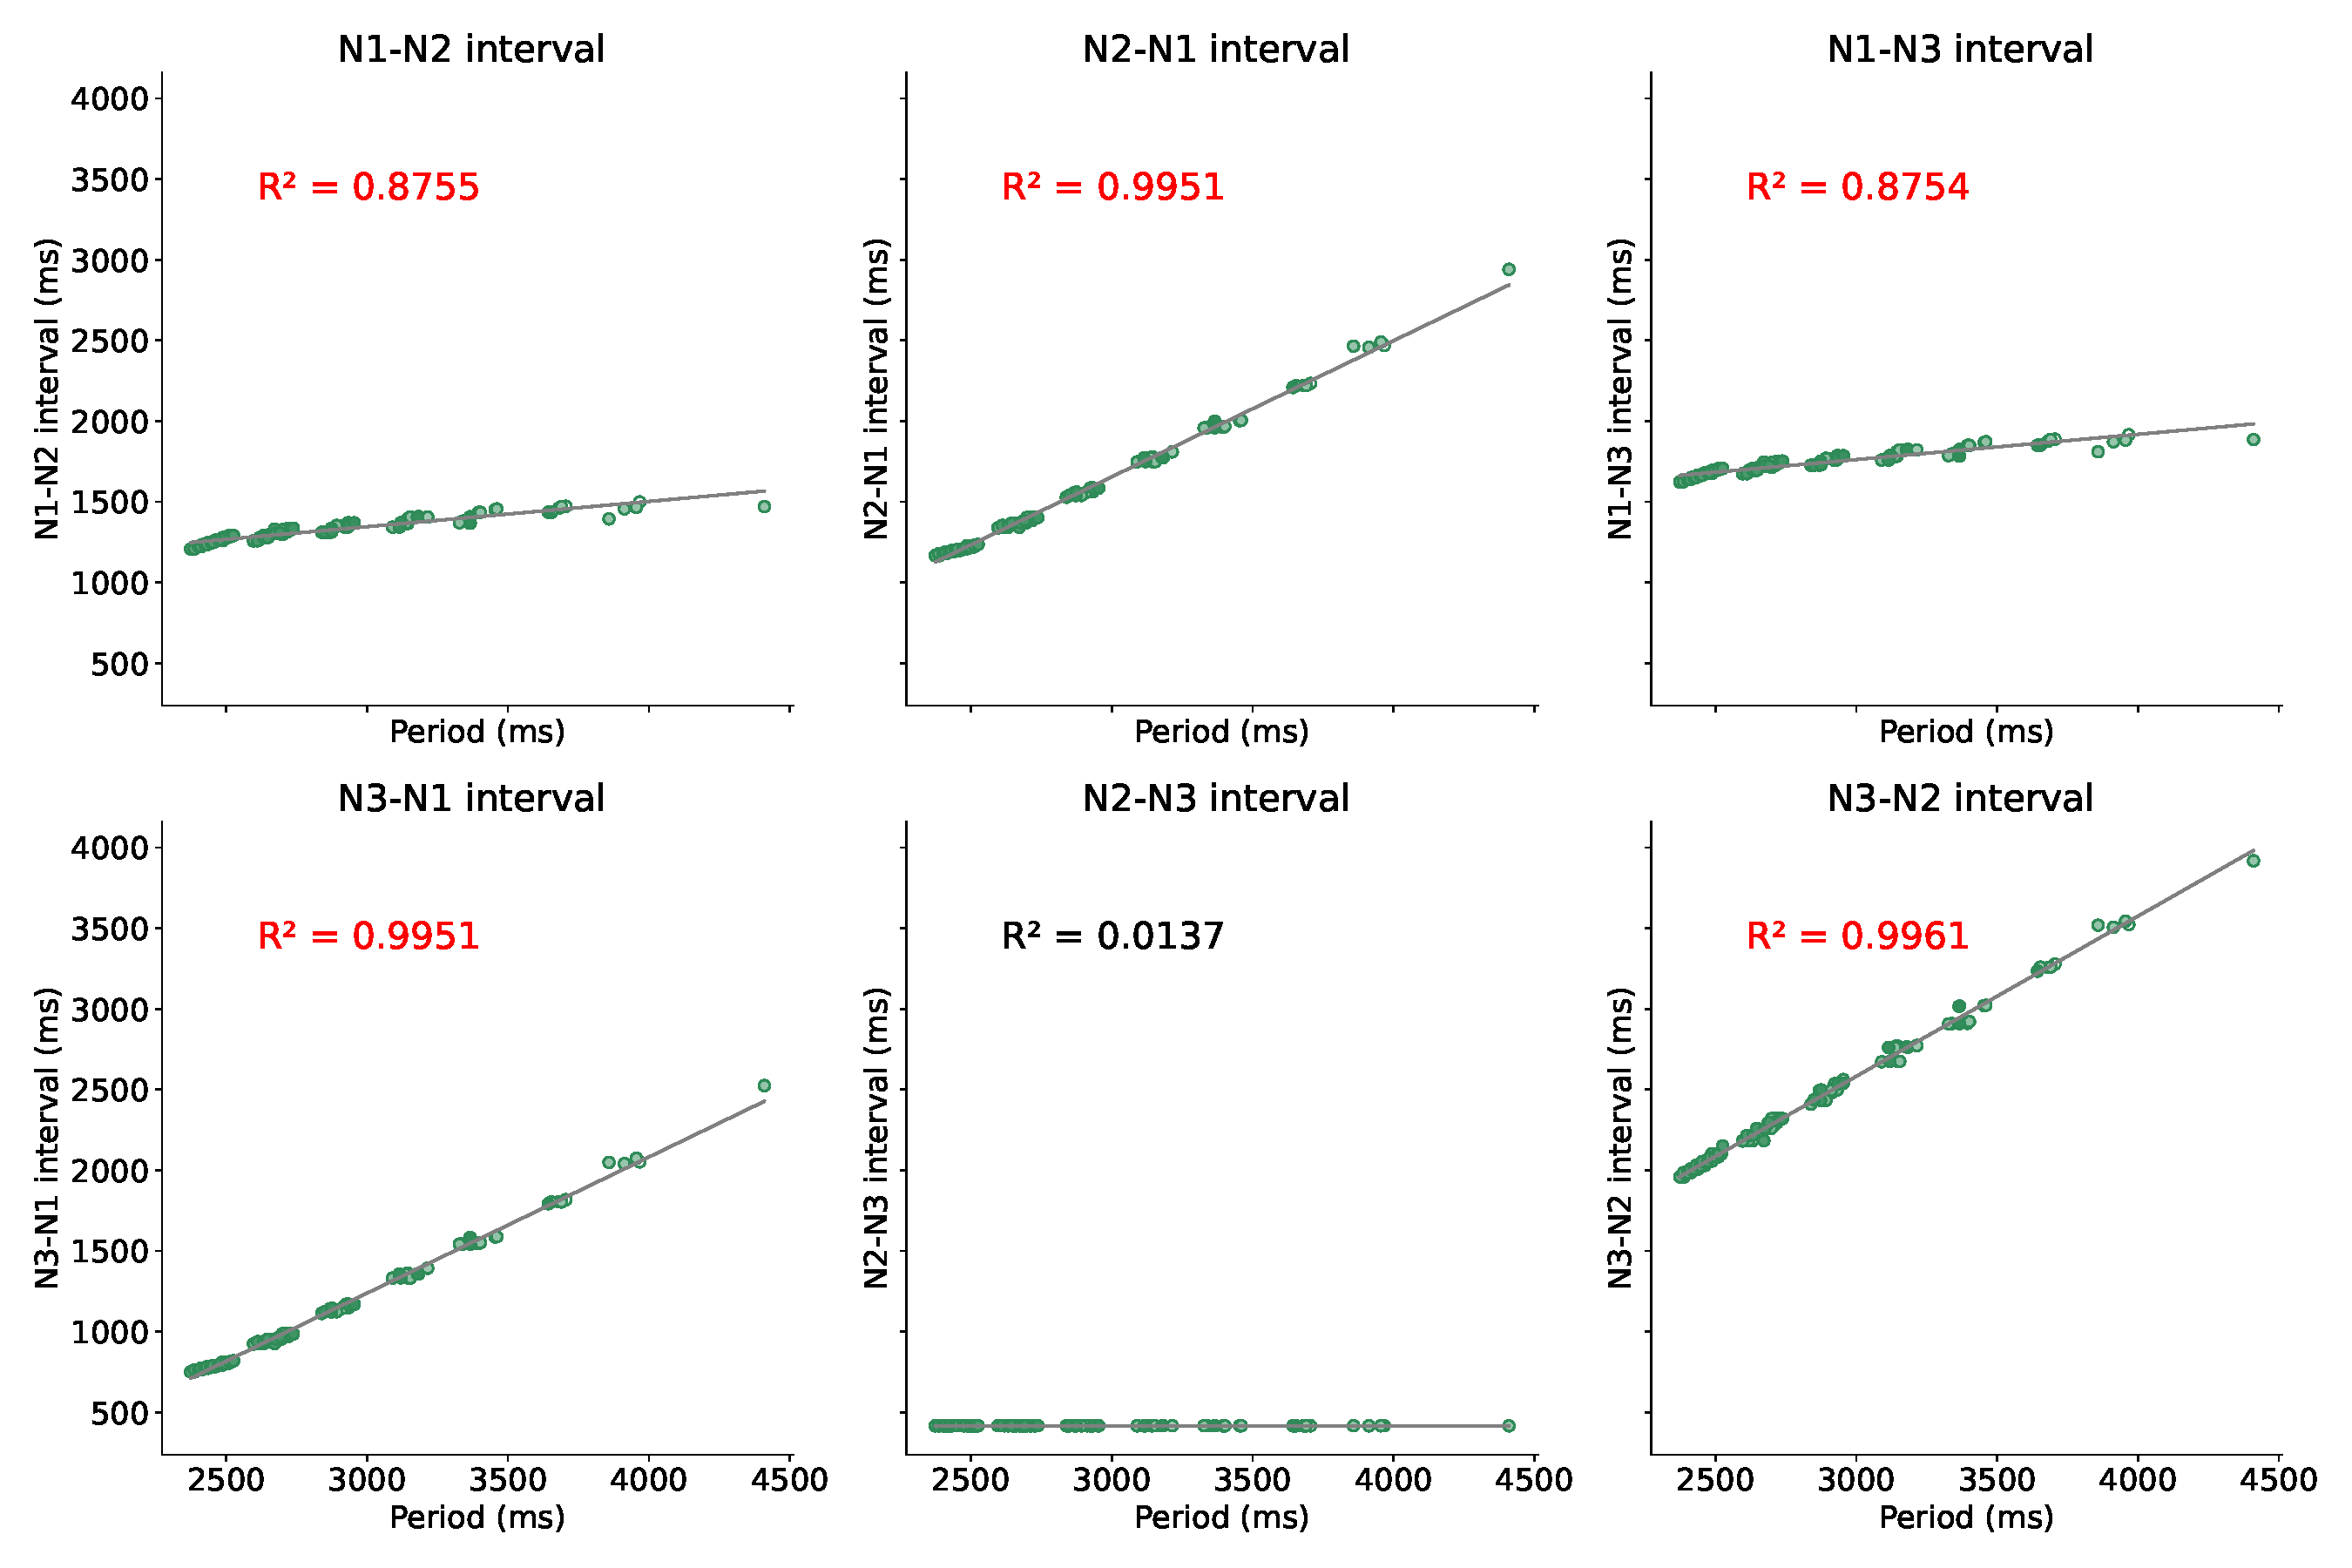
\includegraphics[width=\textwidth]{invariants/data/MODEL/n1m_driven/images/3phases/_intervals.pdf}
			\end{minipage}\
			\begin{minipage}[b]{\textwidth}
				\centering
				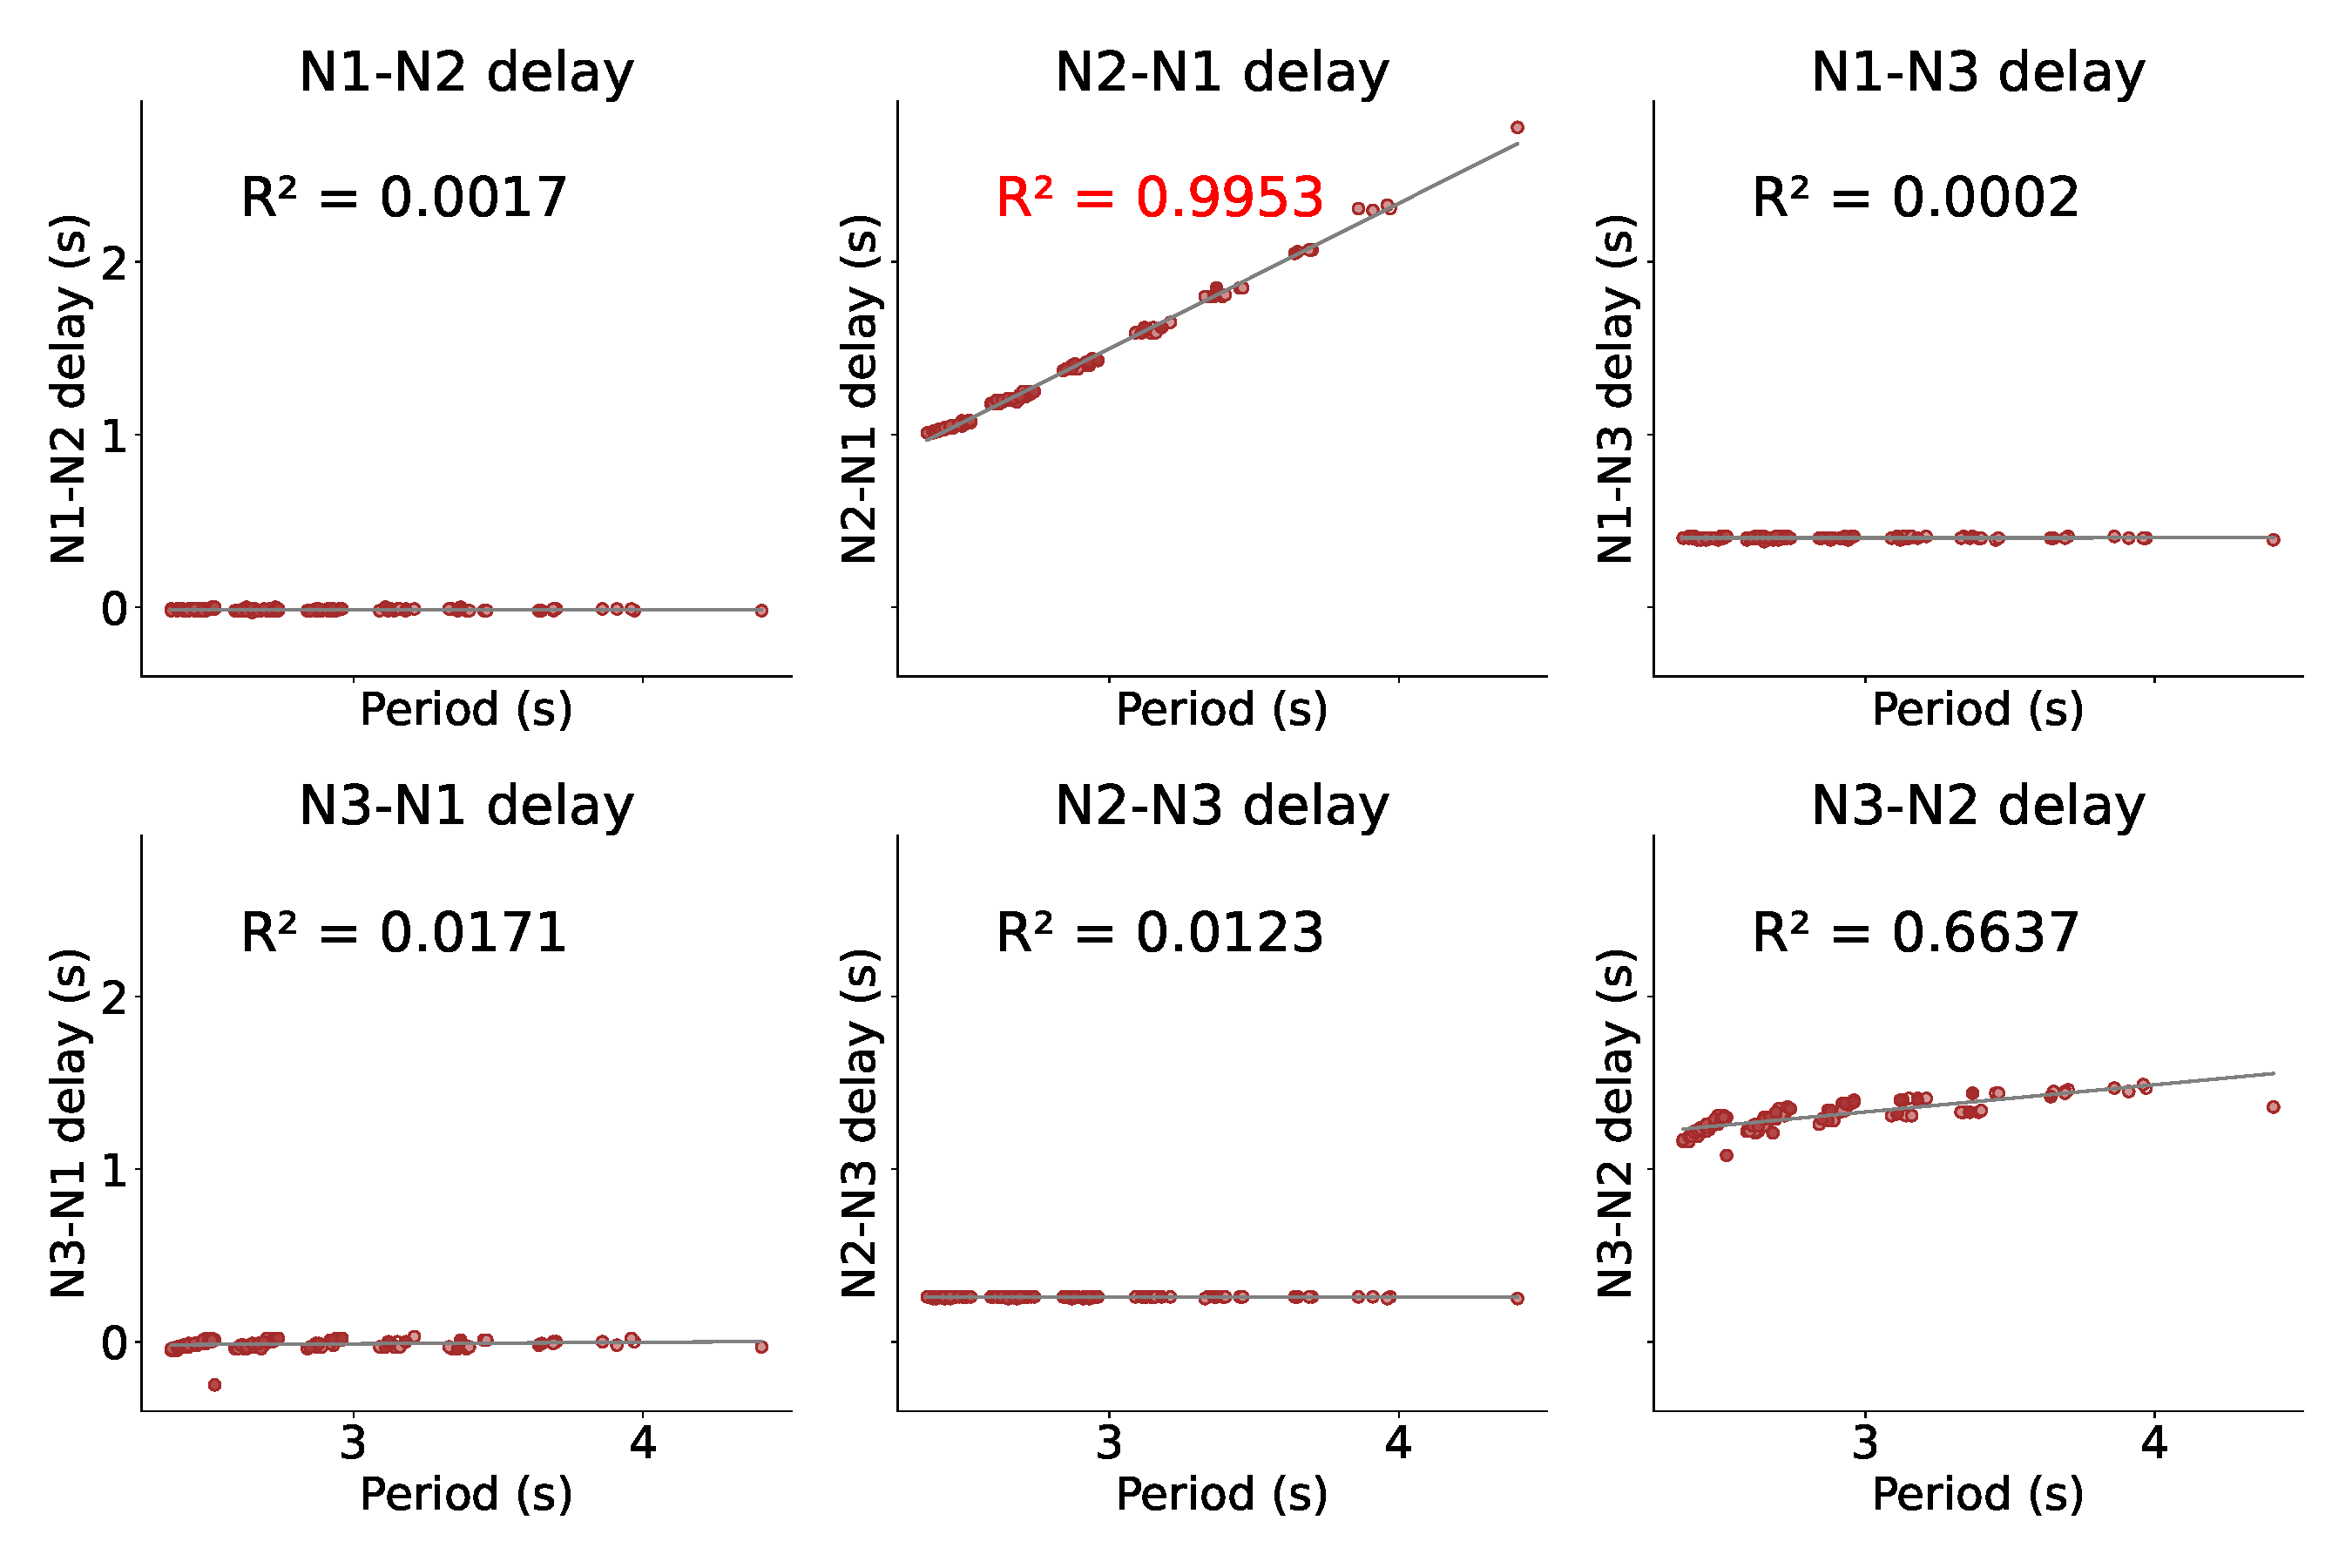
\includegraphics[width=\textwidth]{invariants/data/MODEL/n1m_driven/images/3phases/_delays.pdf}
			\end{minipage}
		\end{minipage}
%		\caption{\textbf{N1M stimulation:} a) Box-plots of the  sequence intervals under N1M neuron stimulation. b) Interval correlations to period for N1M-driven simulation. First row: Burst duration. Second and third row: Two-neuron intervals. Forth and fifth row: Two-neuron delays. Linear relationships are quantified by the $R^2$ values of the linear regression.}
%		\label{fig:invariant n1m}
	\end{figure}
	
\end{frame}


\begin{frame}{SO stimulation}
			
			\begin{figure}[hbt!]
				\begin{minipage}[b]{0.36\textwidth}
					\centering
					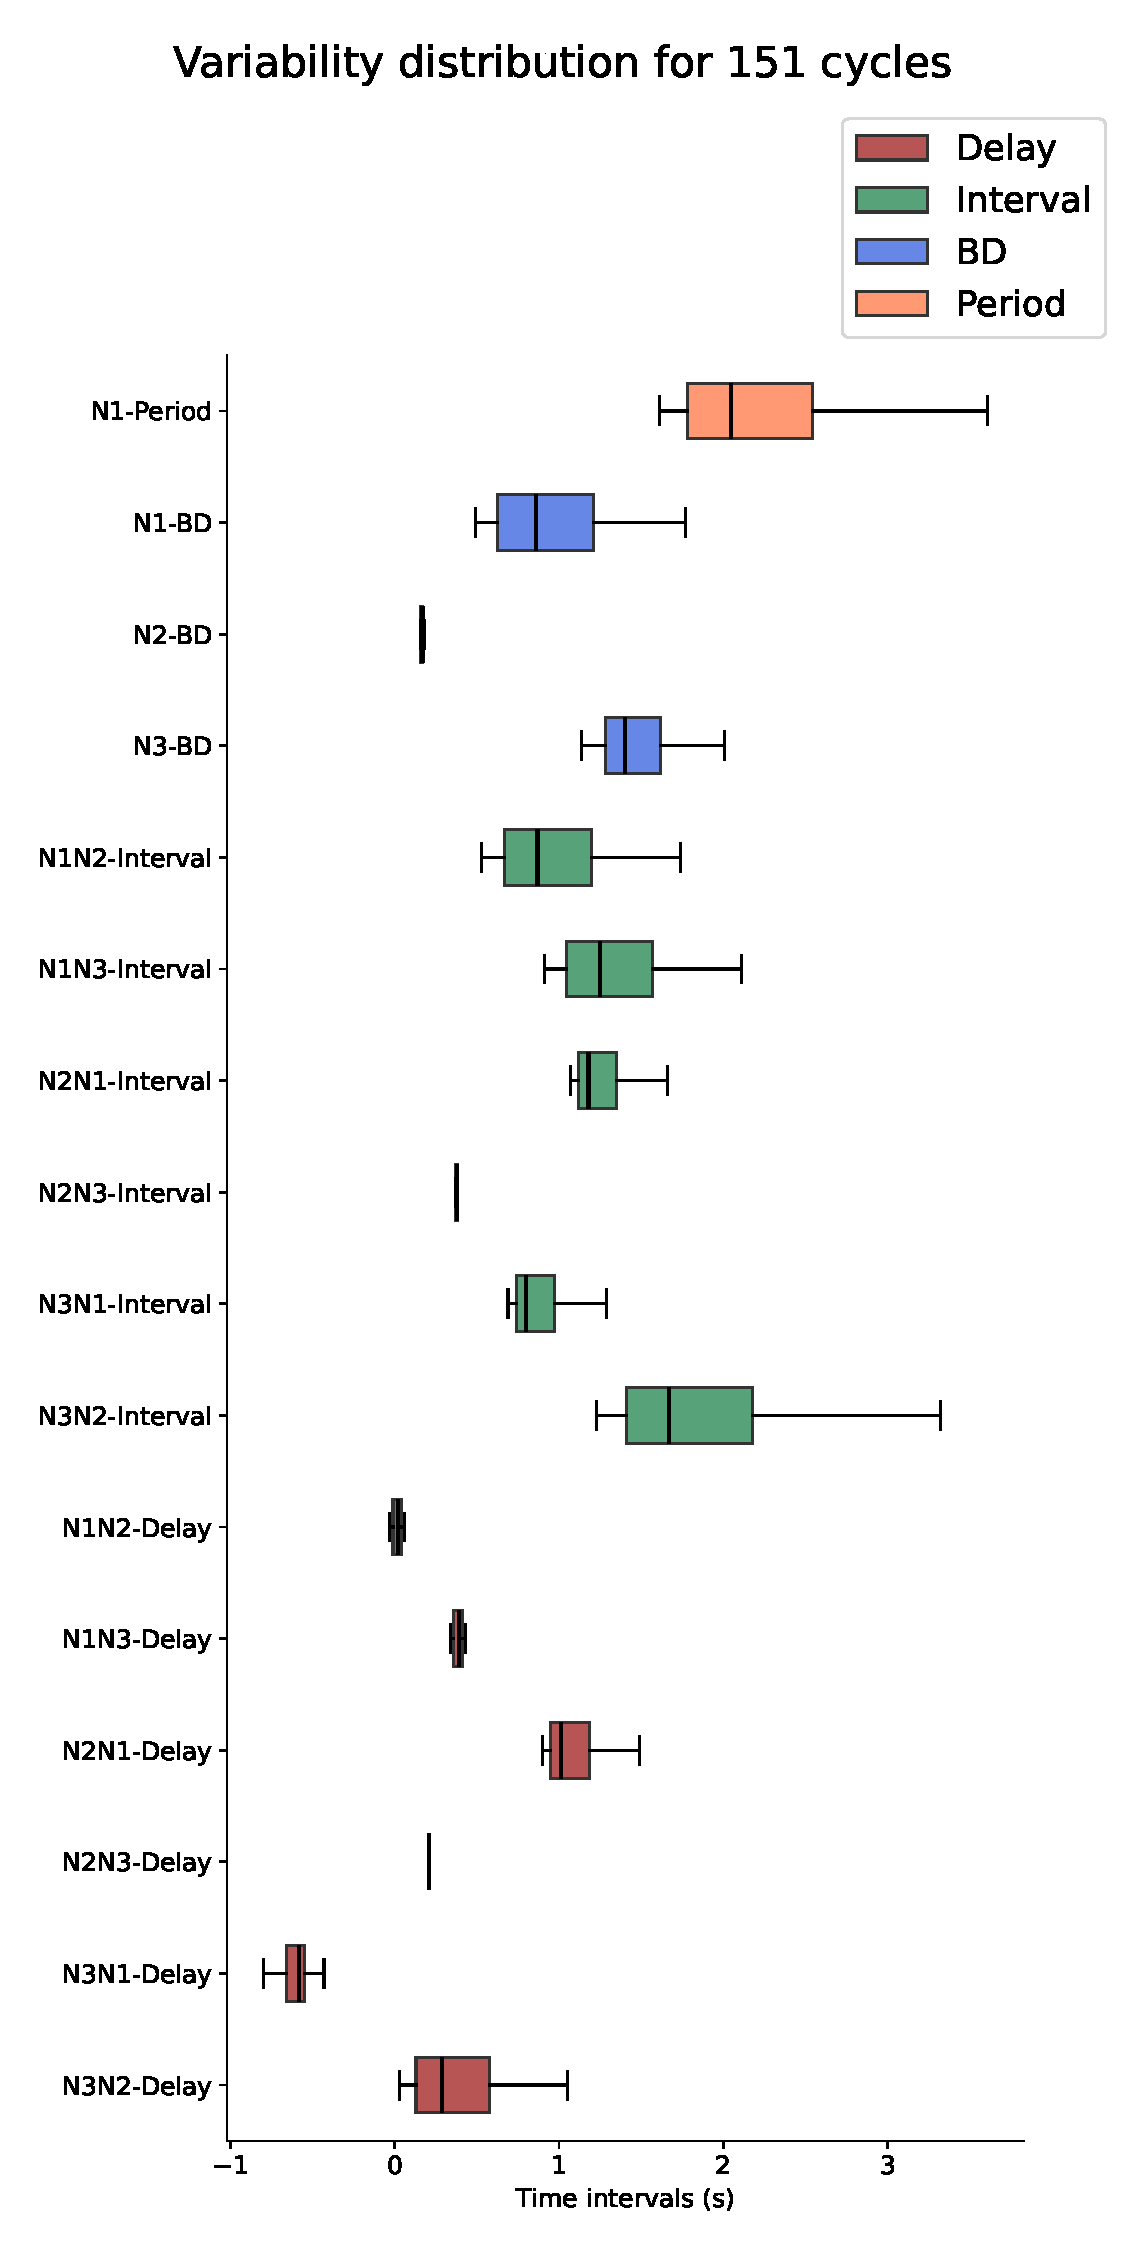
\includegraphics[width=\textwidth]{invariants/data/MODEL/so_driven/images/3phases/_boxplot.pdf}
				\end{minipage}
				\begin{minipage}[b]{0.44\textwidth}
					\centering
					\begin{minipage}[b]{\textwidth}
						\centering
						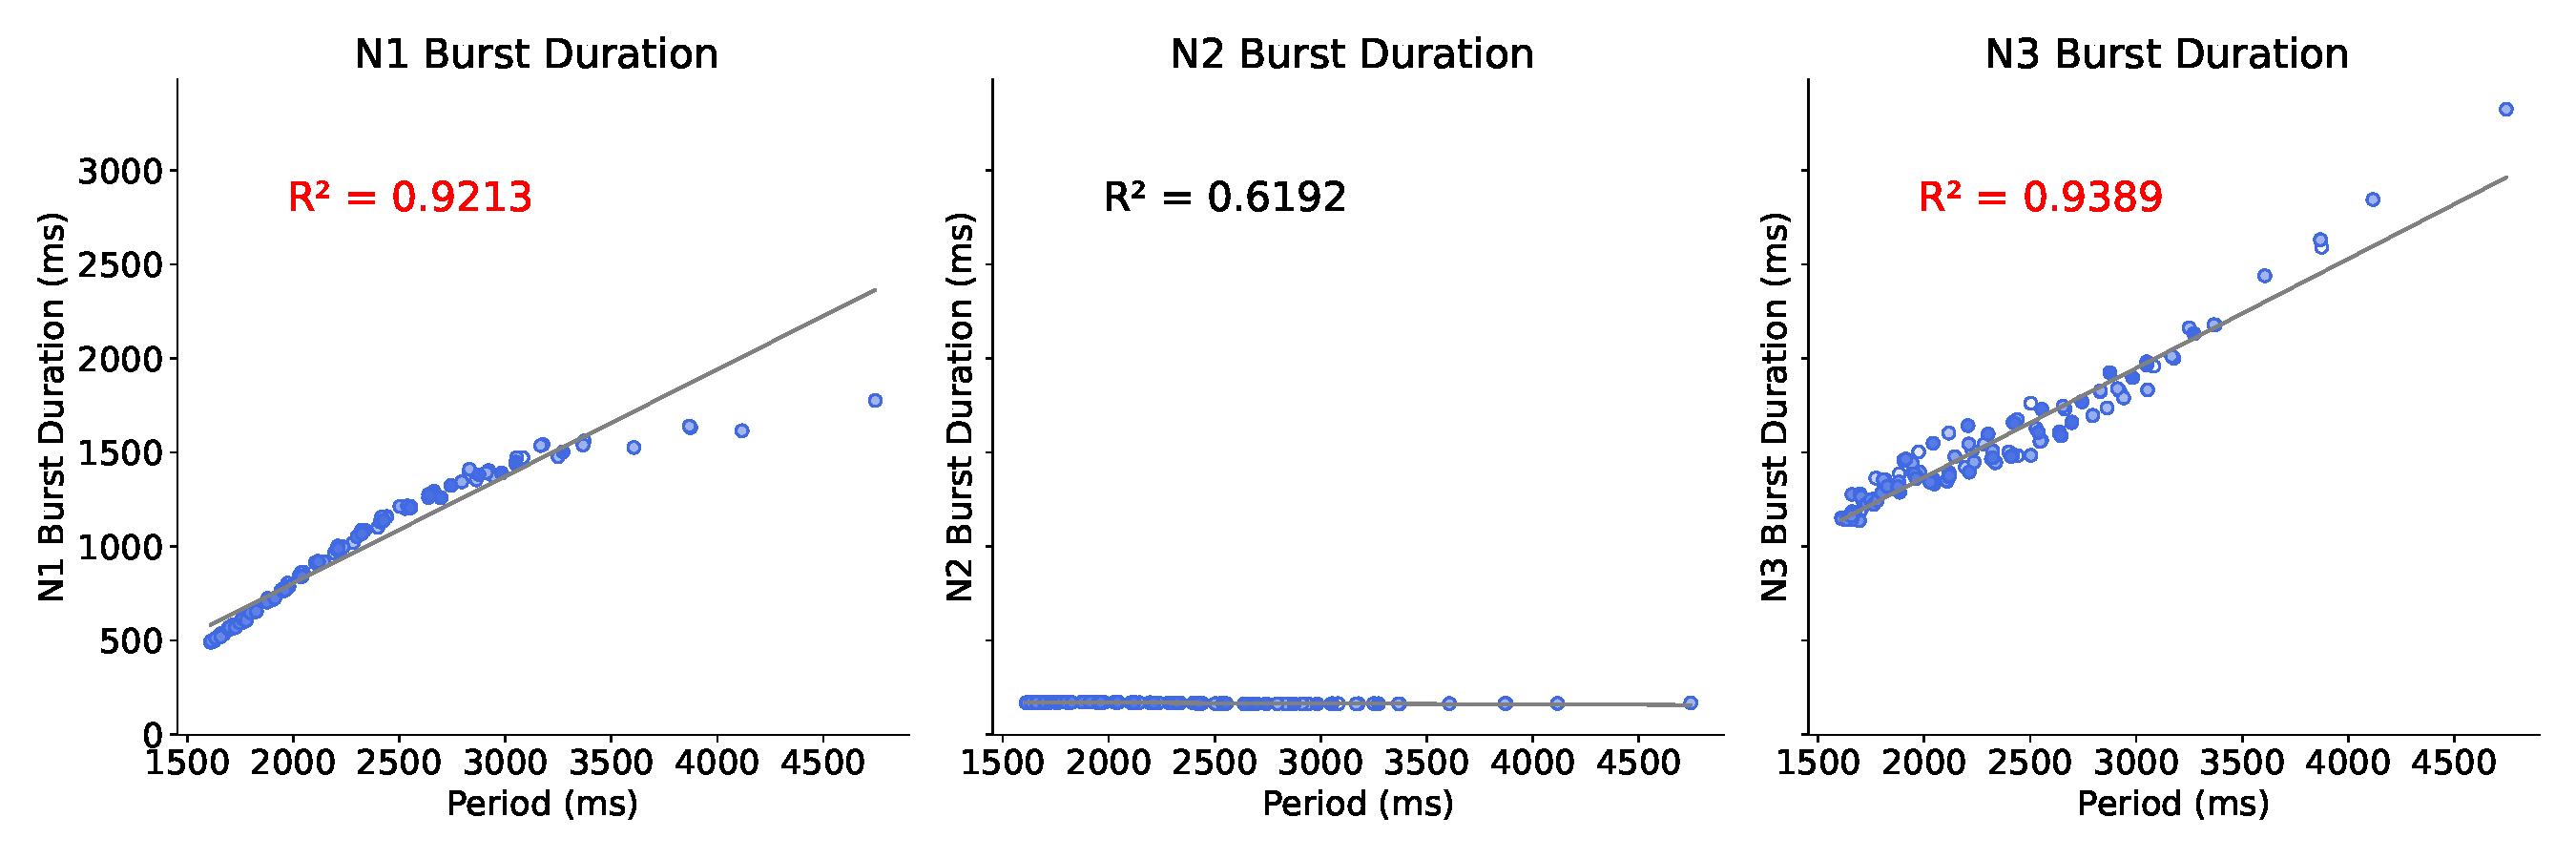
\includegraphics[width=\textwidth]{invariants/data/MODEL/so_driven/images/3phases/_durations.pdf}
					\end{minipage}\
					\begin{minipage}[b]{\textwidth}
						\centering
						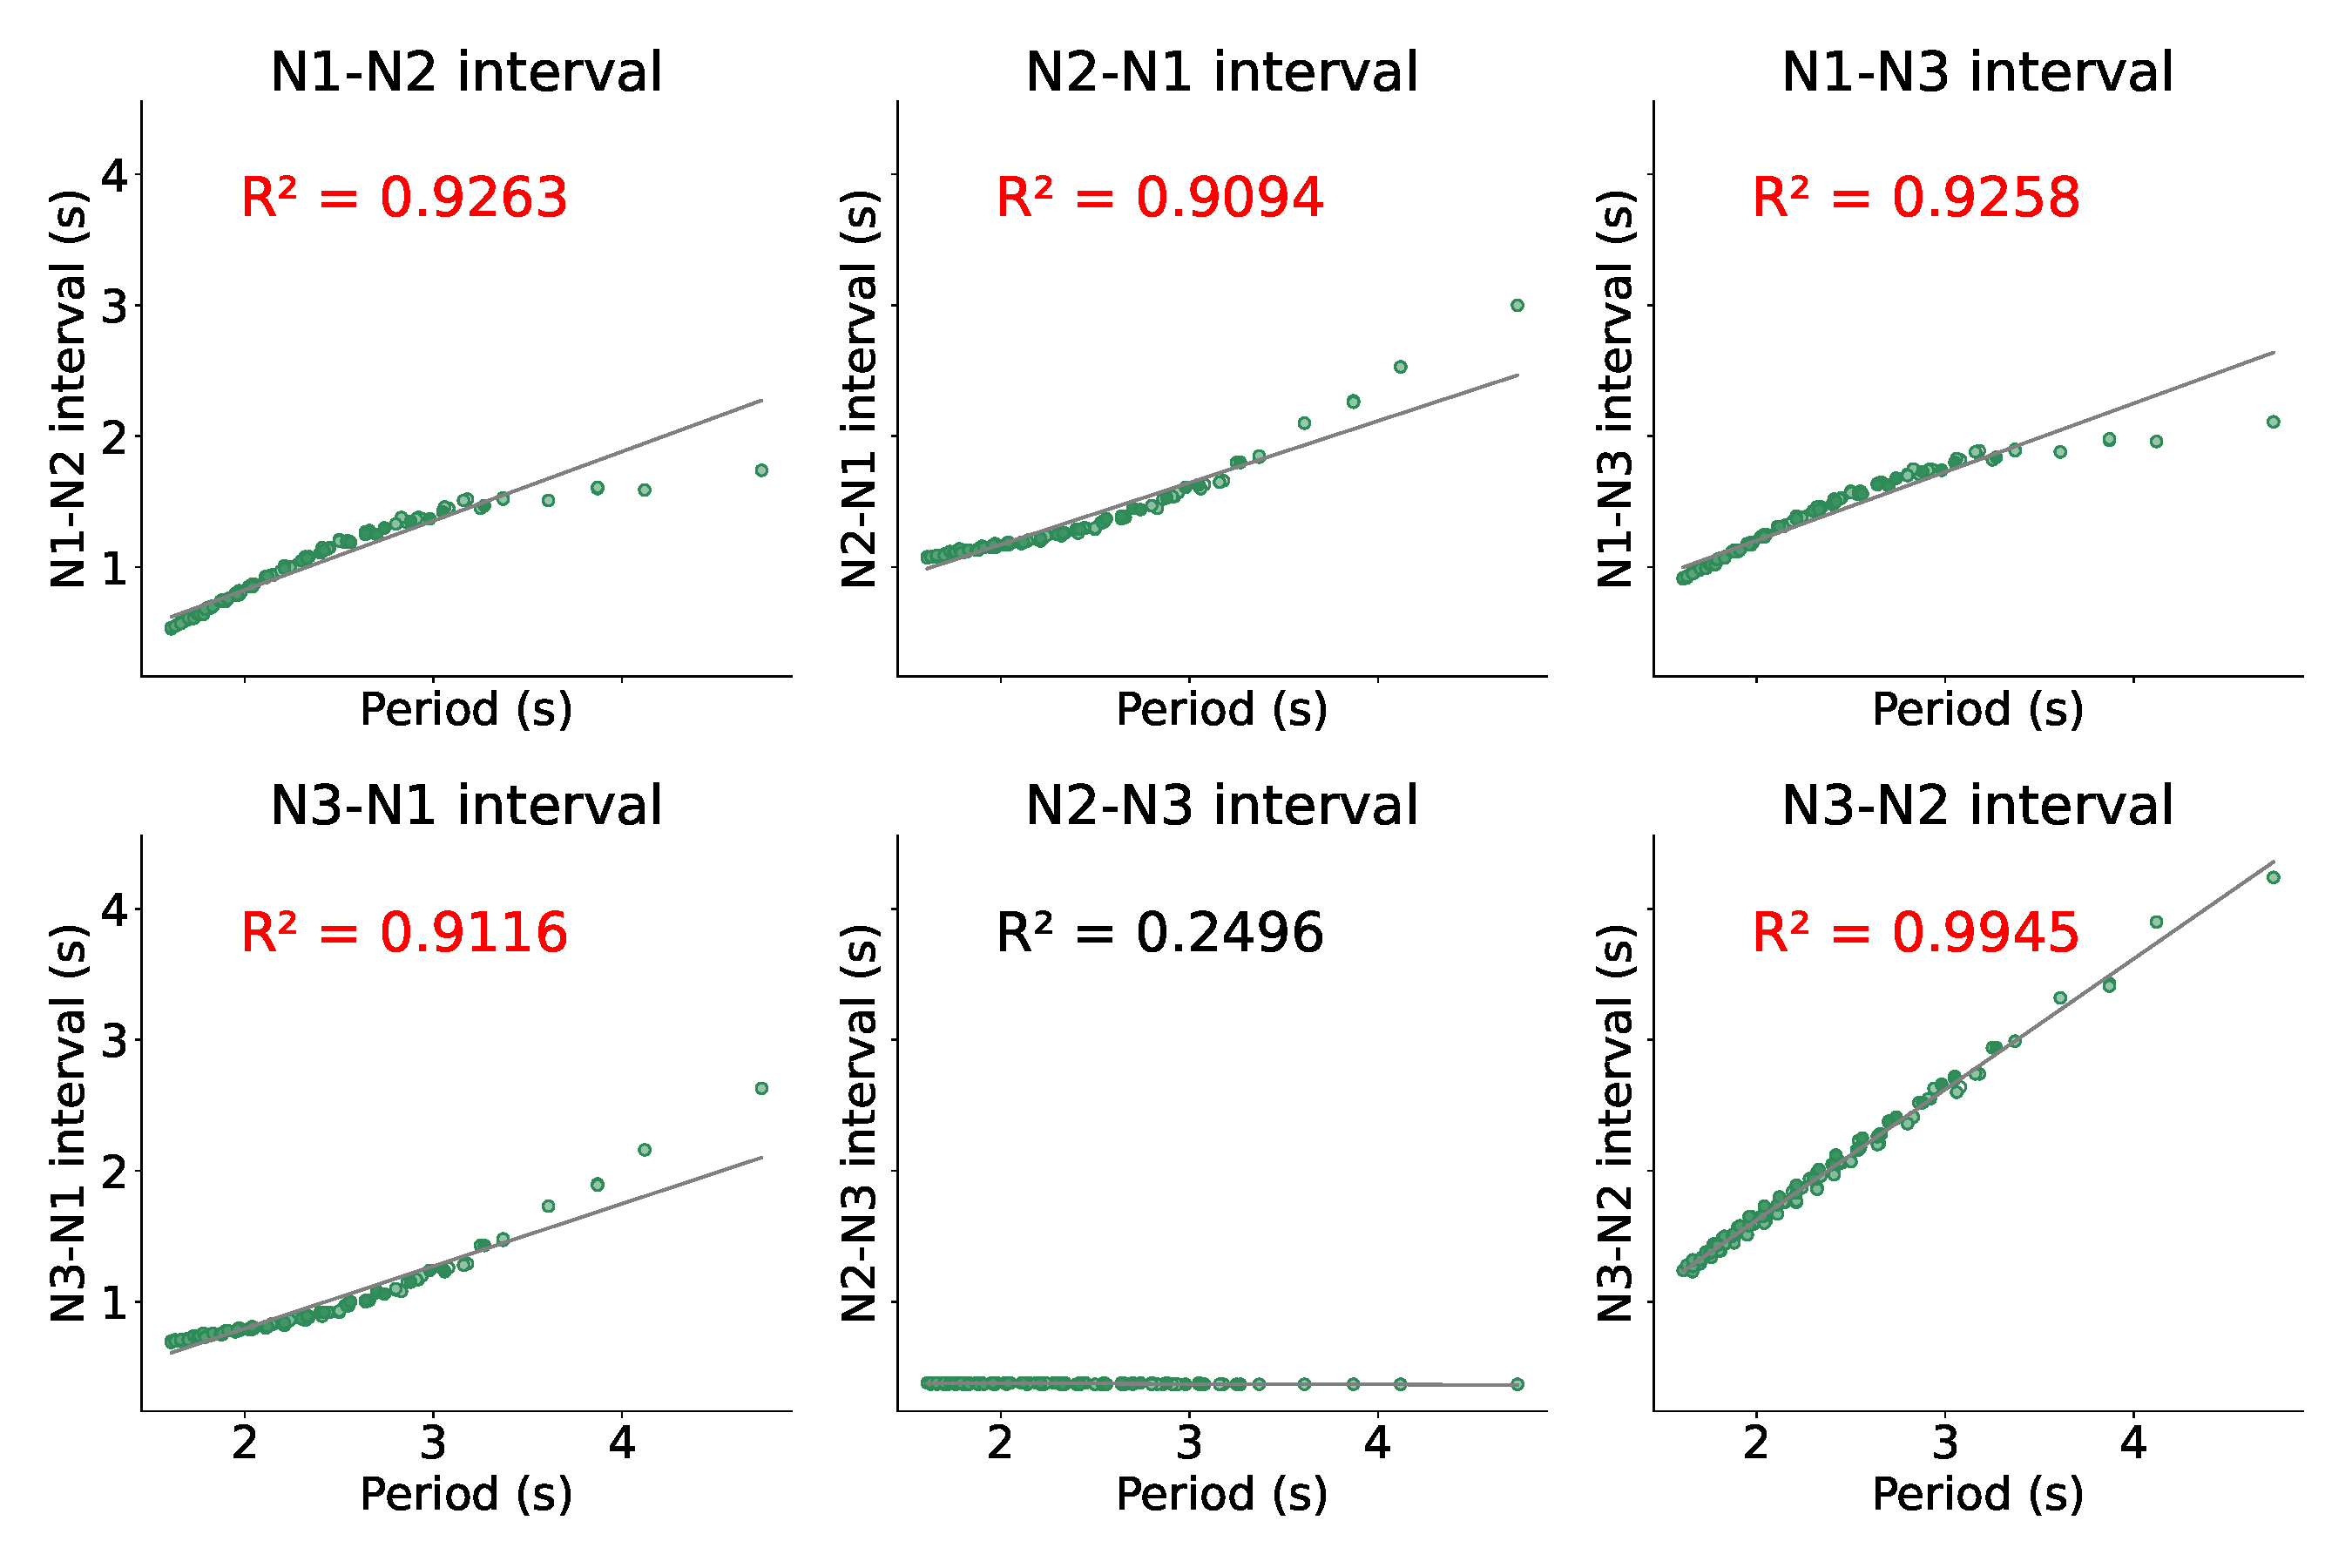
\includegraphics[width=\textwidth]{invariants/data/MODEL/so_driven/images/3phases/_intervals.pdf}
					\end{minipage}\
					\begin{minipage}[b]{\textwidth}
						\centering
						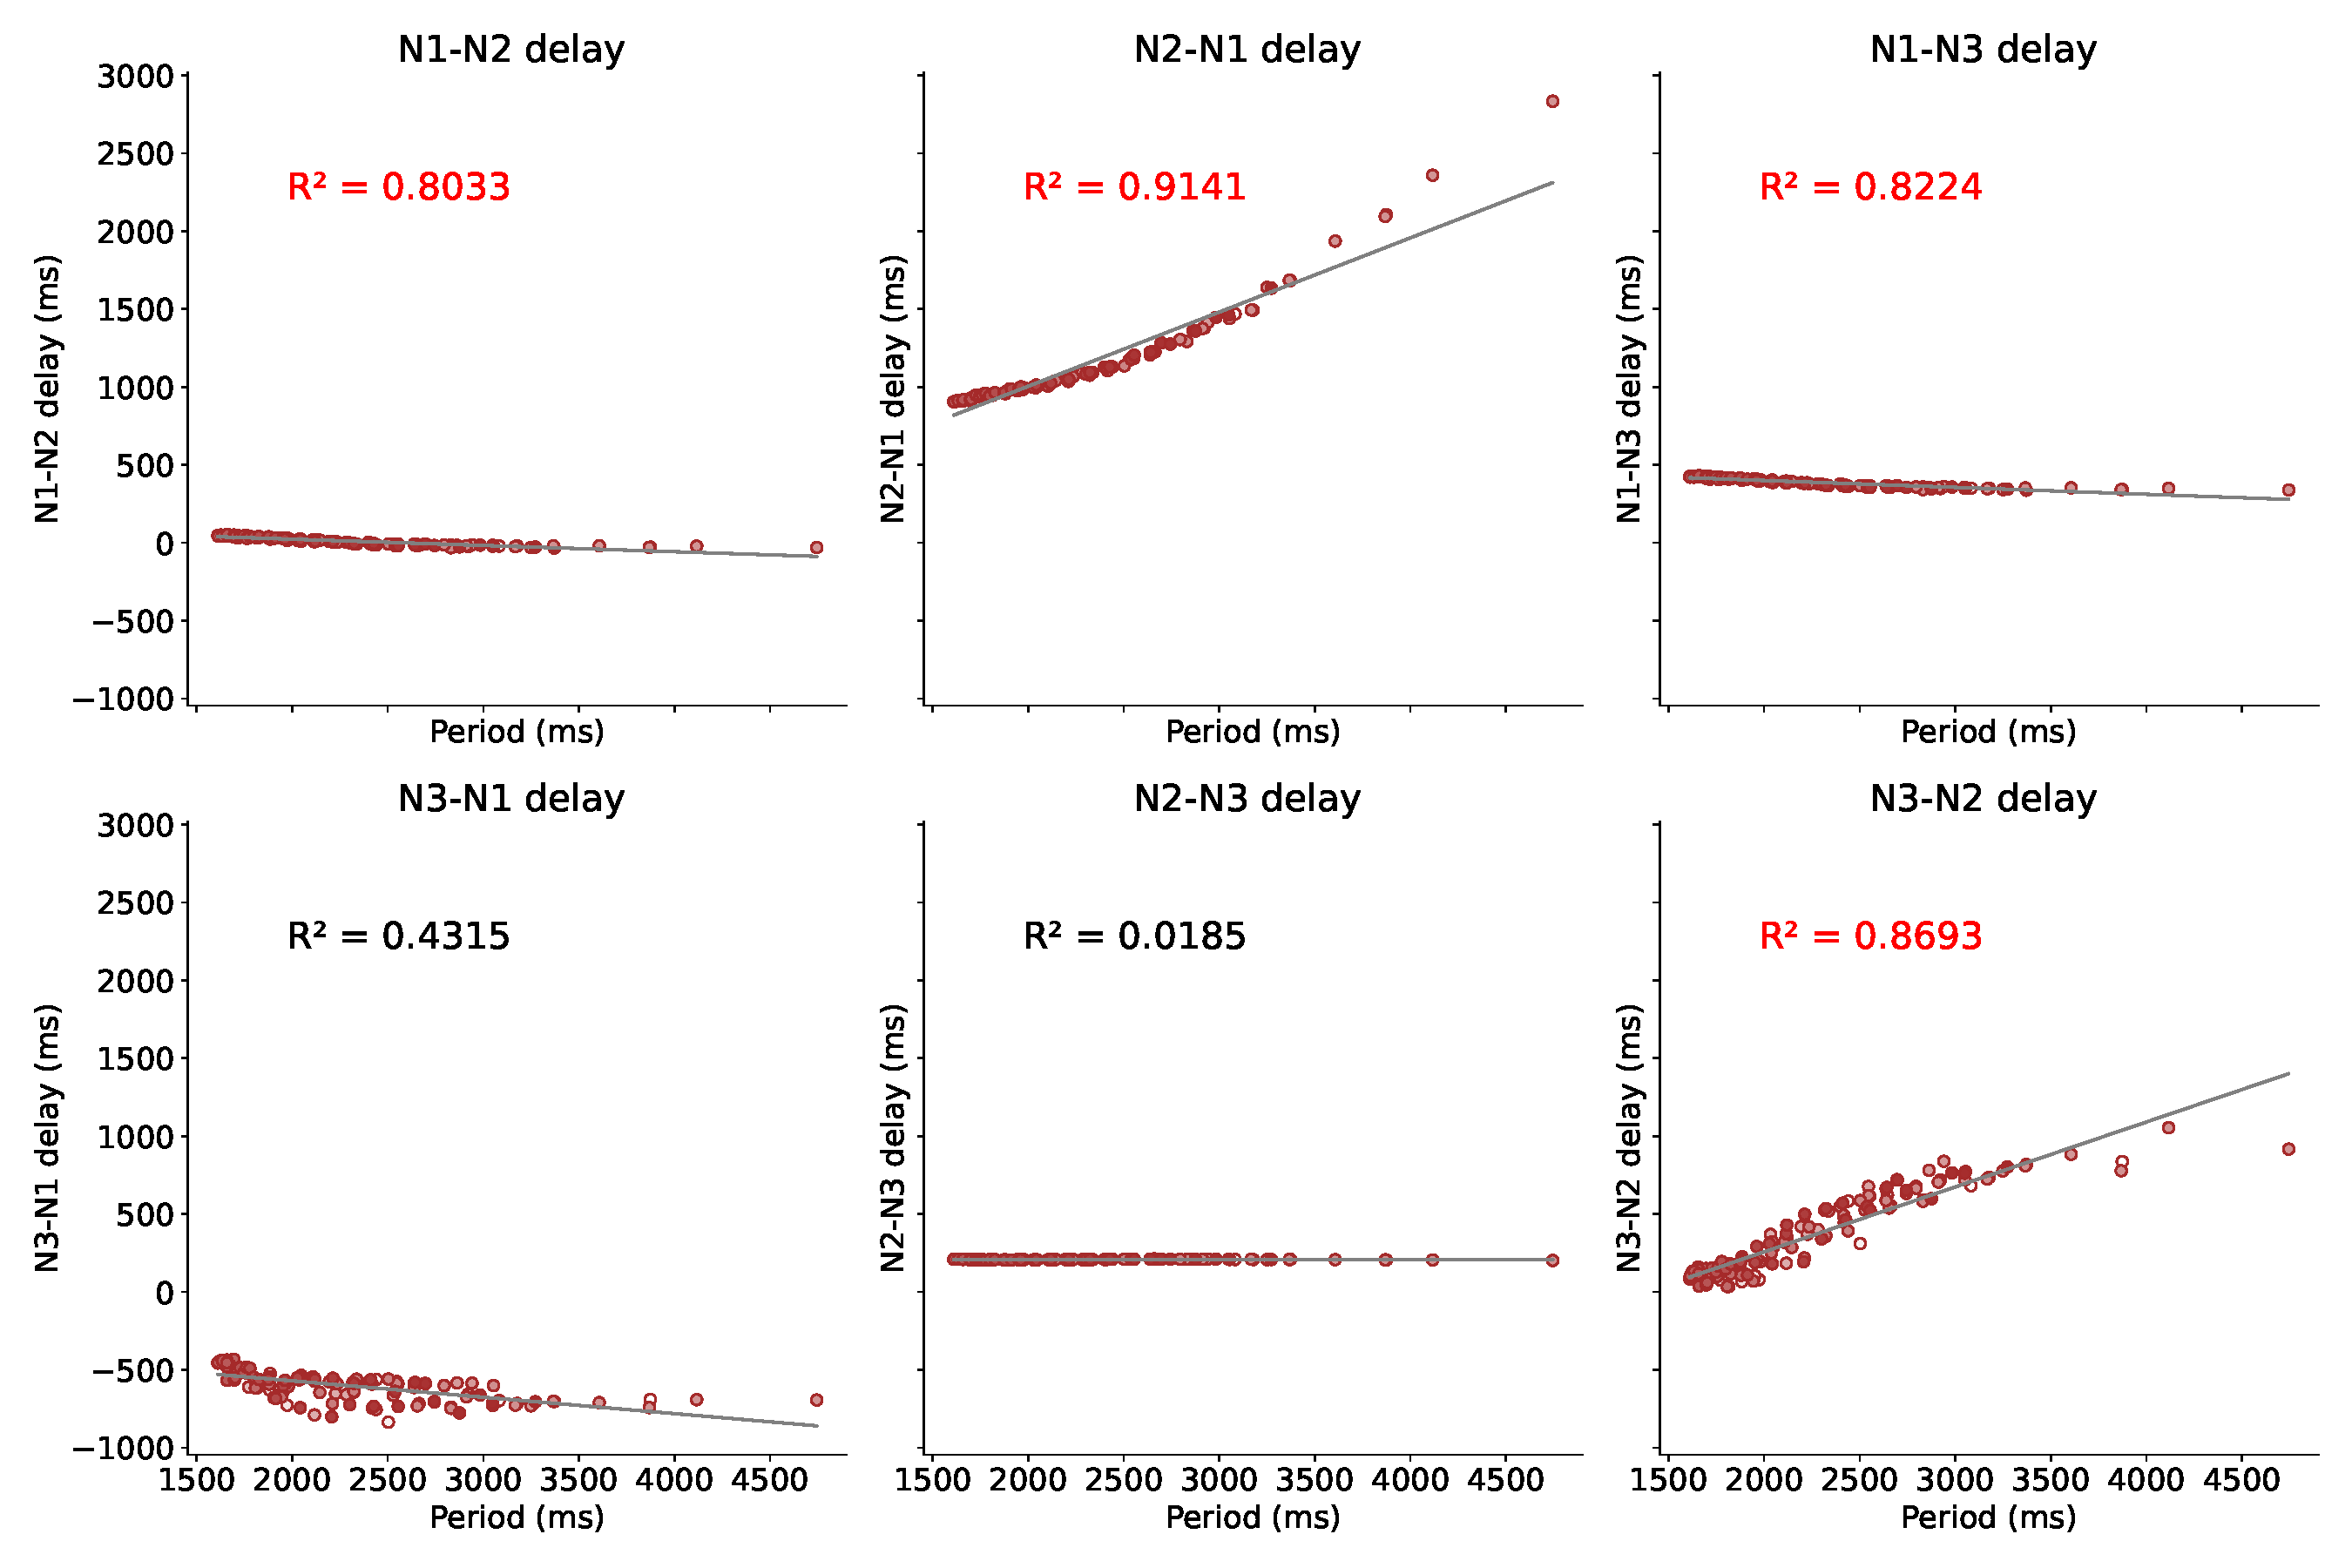
\includegraphics[width=\textwidth]{invariants/data/MODEL/so_driven/images/3phases/_delays.pdf}
					\end{minipage}
				\end{minipage}
%				\caption{\textbf{SO stimulation: }a) Box-plots of the sequence intervals under SO neuron stimulation. b) Interval correlations to Period for SO-driven simulation. First row: Burst duration. Second and third row: Two-neuron intervals. Forth and fifth row: Two-neuron delays.}
%				\label{fig:invariant so}
			\end{figure}
			% TODO probar invariantes cuadrados para ampliar pantalla
			
\end{frame}


\begin{frame}{Models with chaotic activity}
	Variability in models is usually limited. The variability can be induced by a current ramp as in this case, but with a chaotic activity the variability could be more realistic. 
	\vspace{8pt}
	\begin{columns}
		\uncover<2->{
			\begin{column}{0.5\textwidth}
				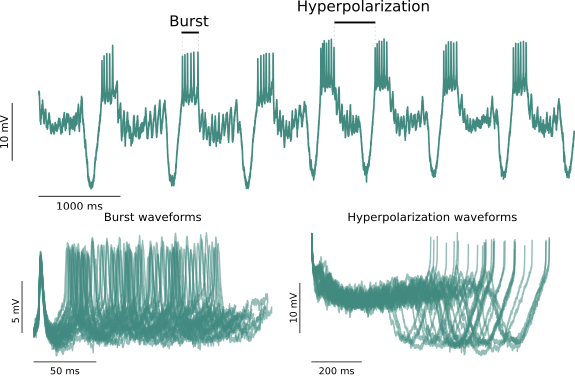
\includegraphics[width=\textwidth]{invariants/variability/lp_burst_variability.png}
				\textbf{Living recording }of LP neuron in the pyloric CPG of \textit{Carcinus maenas}
			\end{column}
		}
		\uncover<3>{
			\begin{column}{0.5\textwidth}
				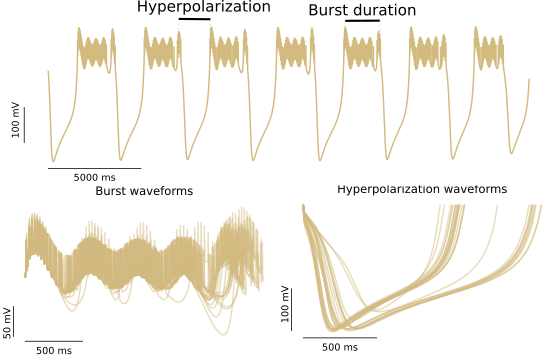
\includegraphics[width=\textwidth]{invariants/variability/TN-burst_variability.png}
				\textbf{Model simulation} with chaotic activity from model Nowotny et al. \textit{PlosOne}(2008)
			\end{column}
		}
	\end{columns}
	%TODO DONE añadir "registro LP" y Nowotny et al. 
\end{frame}



\begin{frame}{Experimental approach}
	\only<1-2>{
	\begin{itemize}
		\item<1-2>Are sequential invariants present also in the experimental recordings? 
		\item<2-2>Do the invariants change under different stimulation conditions?
	\end{itemize}
}		
		\only<3->{
			Previous studies point to the linear relation between some phases and the period 
			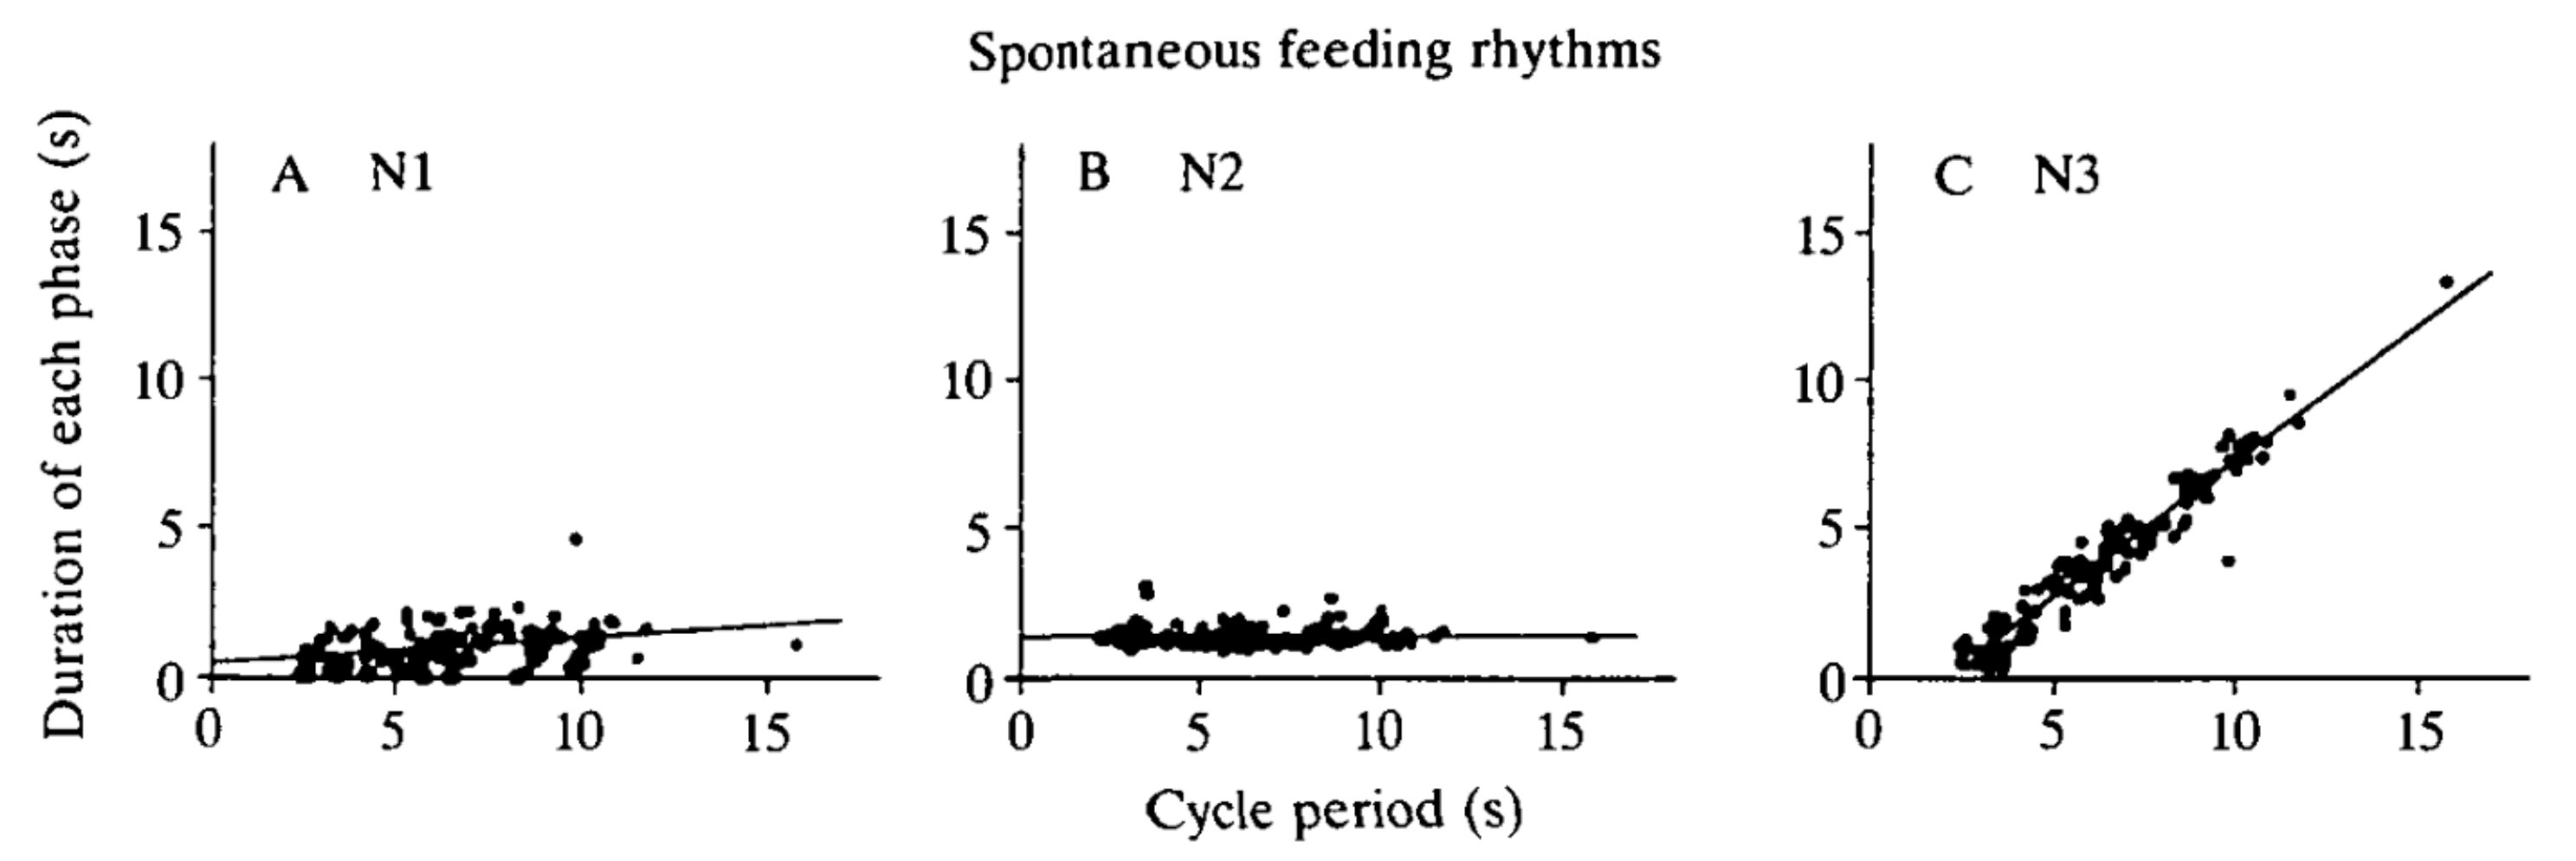
\includegraphics[width=\linewidth]{Images/elliot_n_andrew.png}
			\tiny{Elliott, C. J. H., \& Andrew, T. (1991). Temporal Analysis of Snail Feeding Rhythms: A Three-Phase Relaxation Oscillator. Journal of Experimental Biology, 157(1), 391–408. Figure 5.}
		}
	\note{WE ANALYZE ALL INTERVALS, dejar clara aportación
	Linear relationships with the interval -> linear relatioships with the cycle period 
}
	%TODO separar en dos
	
	
\end{frame}

\begin{frame}{Distributed neural system of \textit{L. stagnalis}}
	\only<1>{
		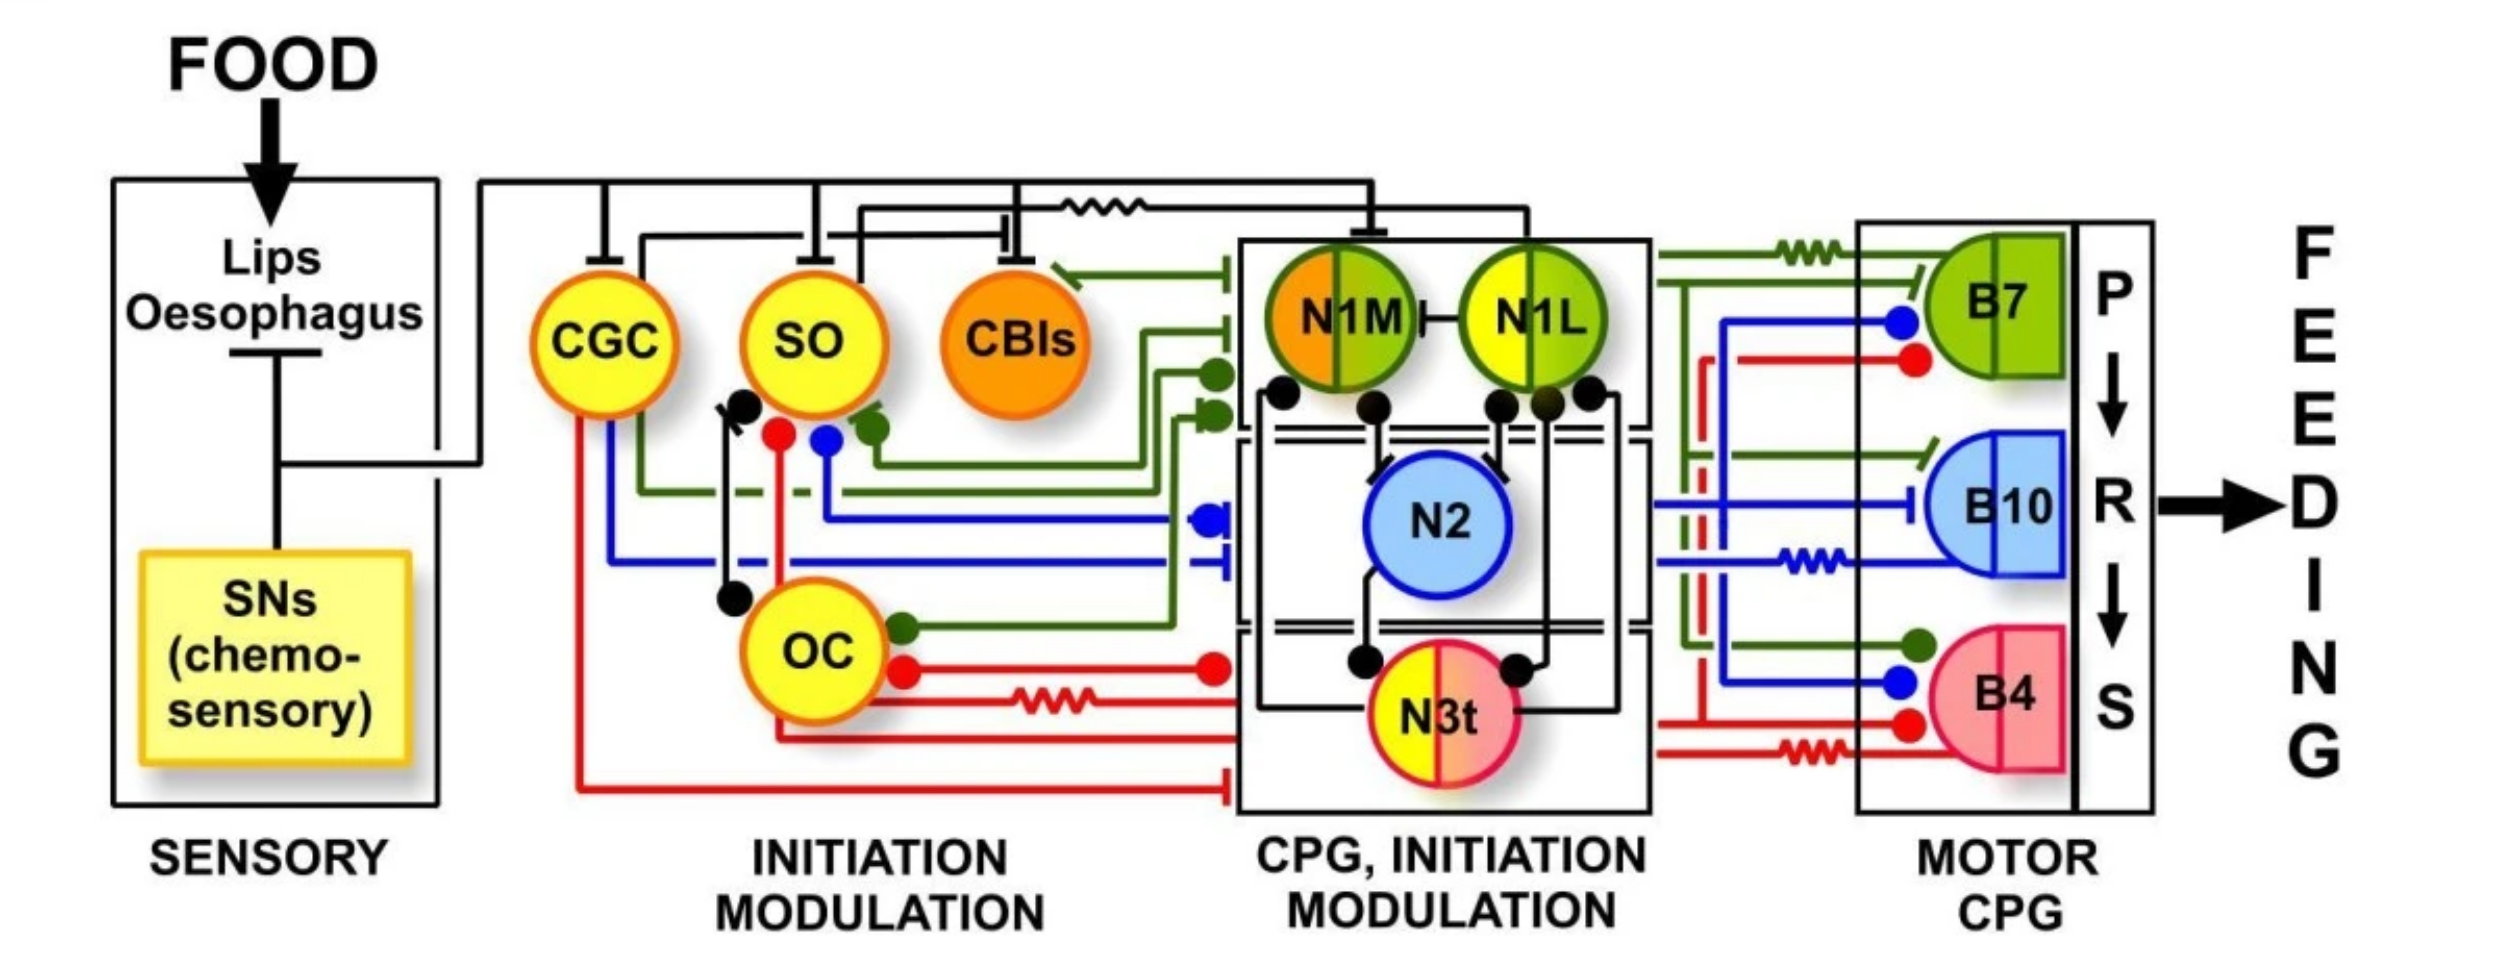
\includegraphics[width=\textwidth]{invariants/distributed_benjamin_2012.png}
		\tiny{Benjamin, P. R. (2012). Distributed network organization underlying feeding behavior in the mollusk Lymnaea. Neural Systems \& Circuits, 2(1), 1–16. https://doi.org/10.1186/2042-1001-2-4}
			
	}

	\only<2>{
		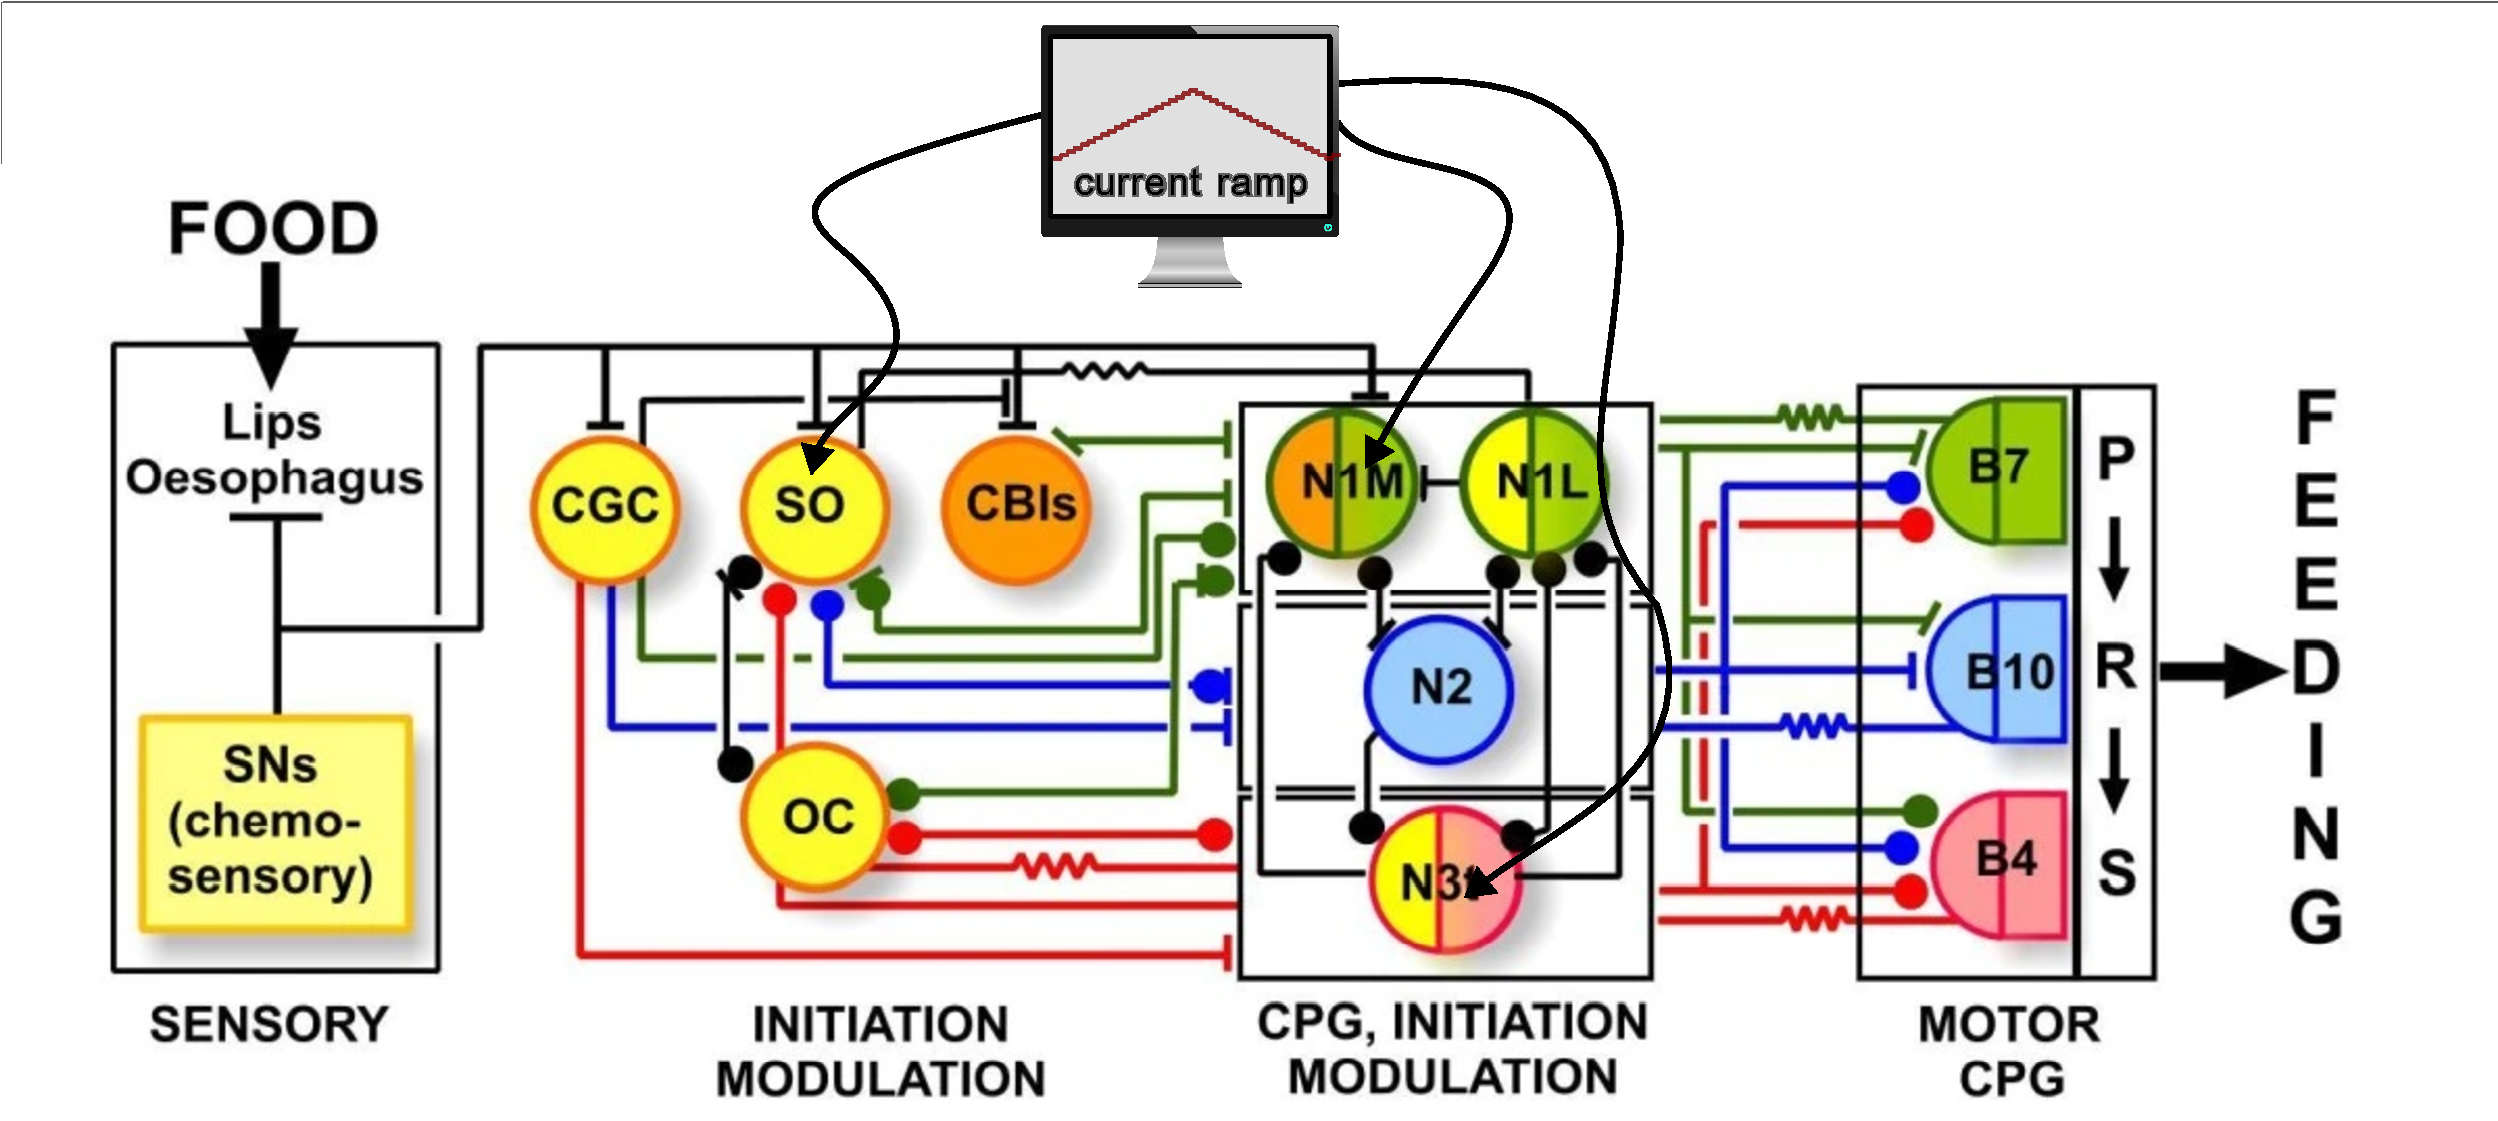
\includegraphics[width=\textwidth]{Images/distributed_benjamin_2012_modelstim.pdf}
		\tiny{Benjamin, P. R. (2012). Distributed network organization underlying feeding behavior in the mollusk Lymnaea. Neural Systems \& Circuits, 2(1), 1–16. https://doi.org/10.1186/2042-1001-2-4}
	}


	\only<3>{
		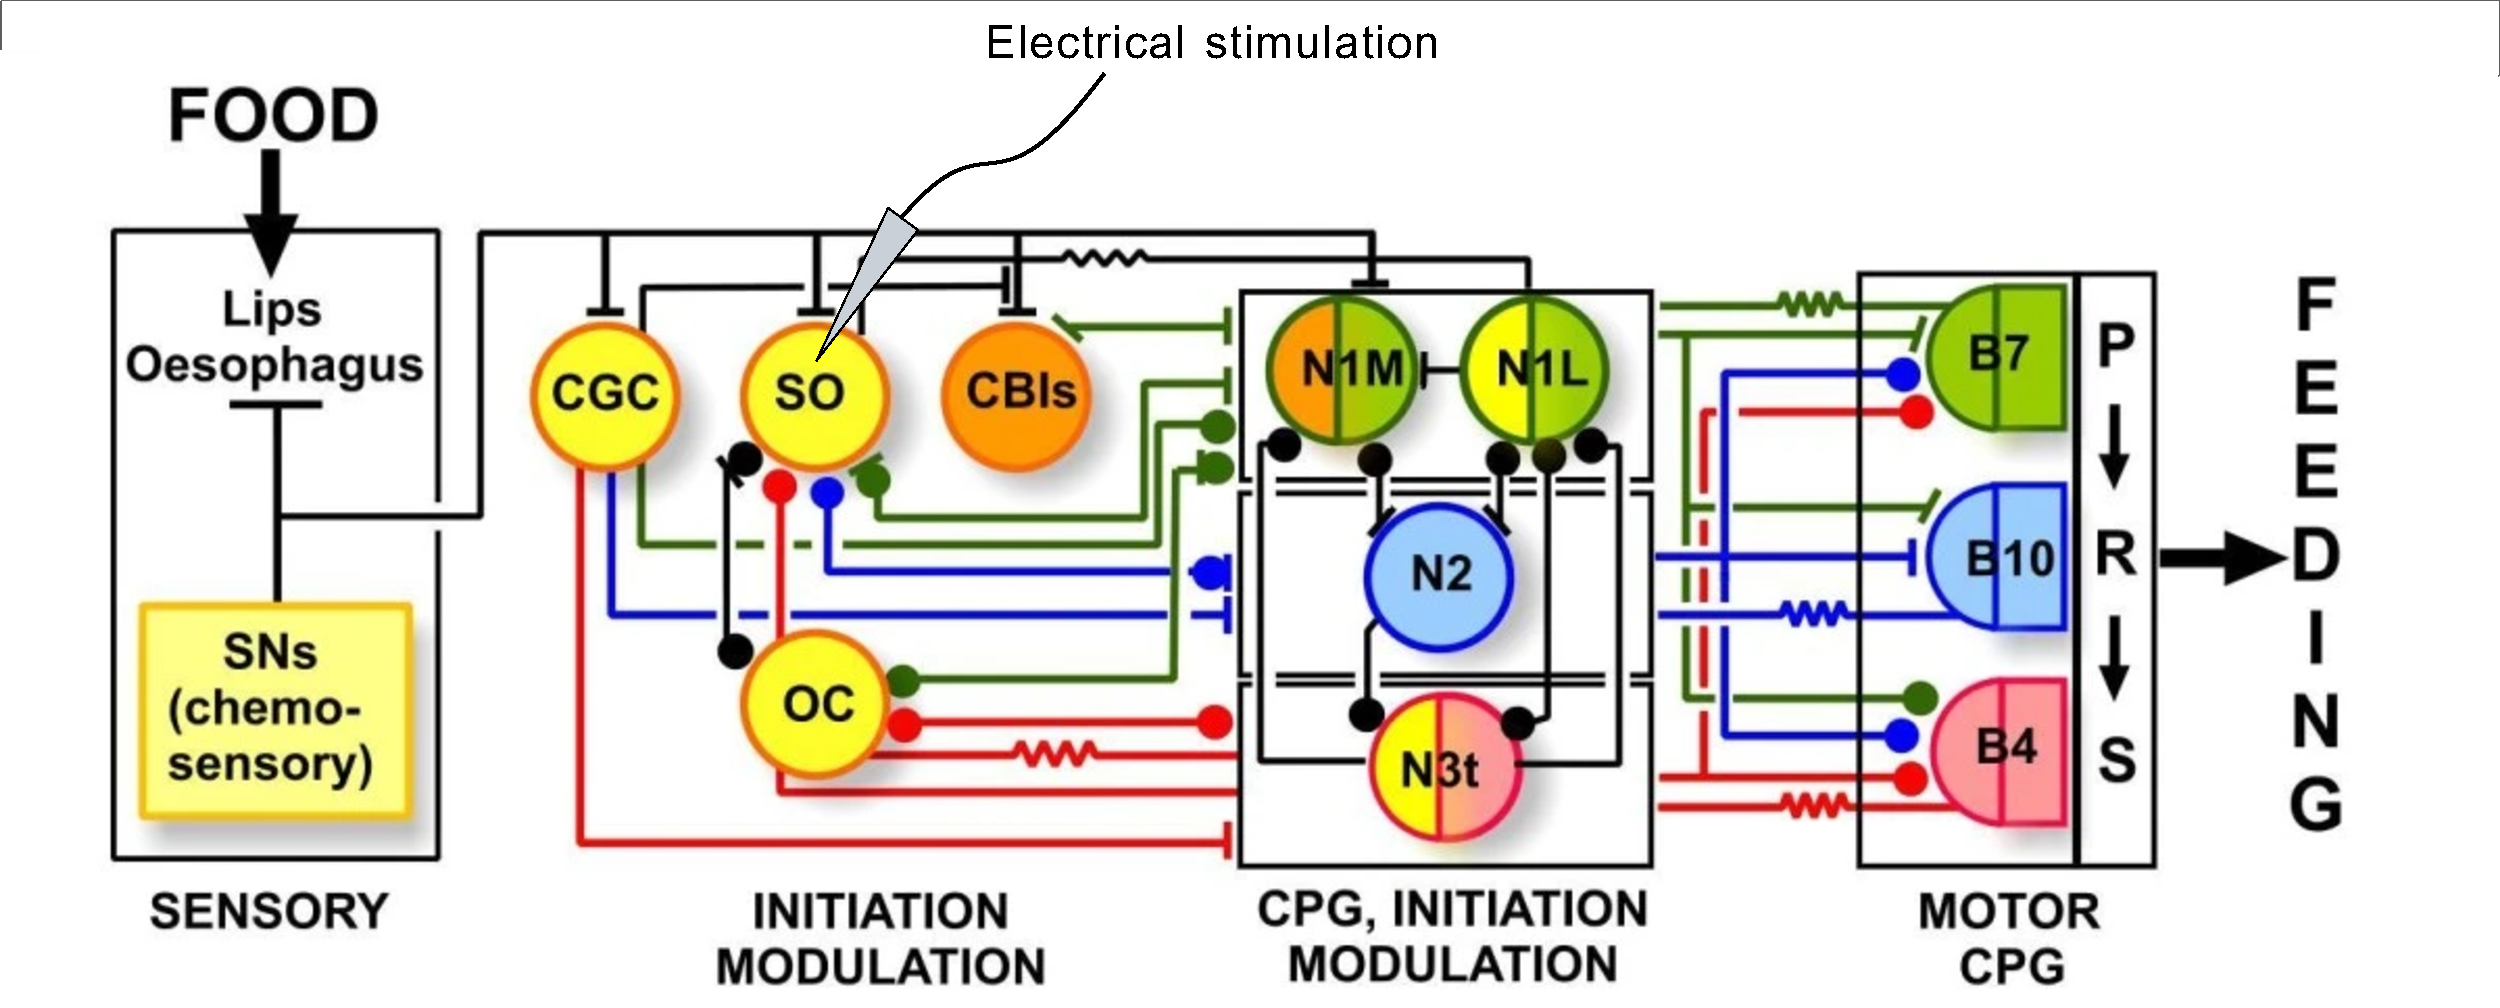
\includegraphics[width=\textwidth]{Images/distributed_benjamin_2012_electrophys_so.pdf}
		\tiny{Benjamin, P. R. (2012). Distributed network organization underlying feeding behavior in the mollusk Lymnaea. Neural Systems \& Circuits, 2(1), 1–16. https://doi.org/10.1186/2042-1001-2-4}
	}
	\only<4>{
	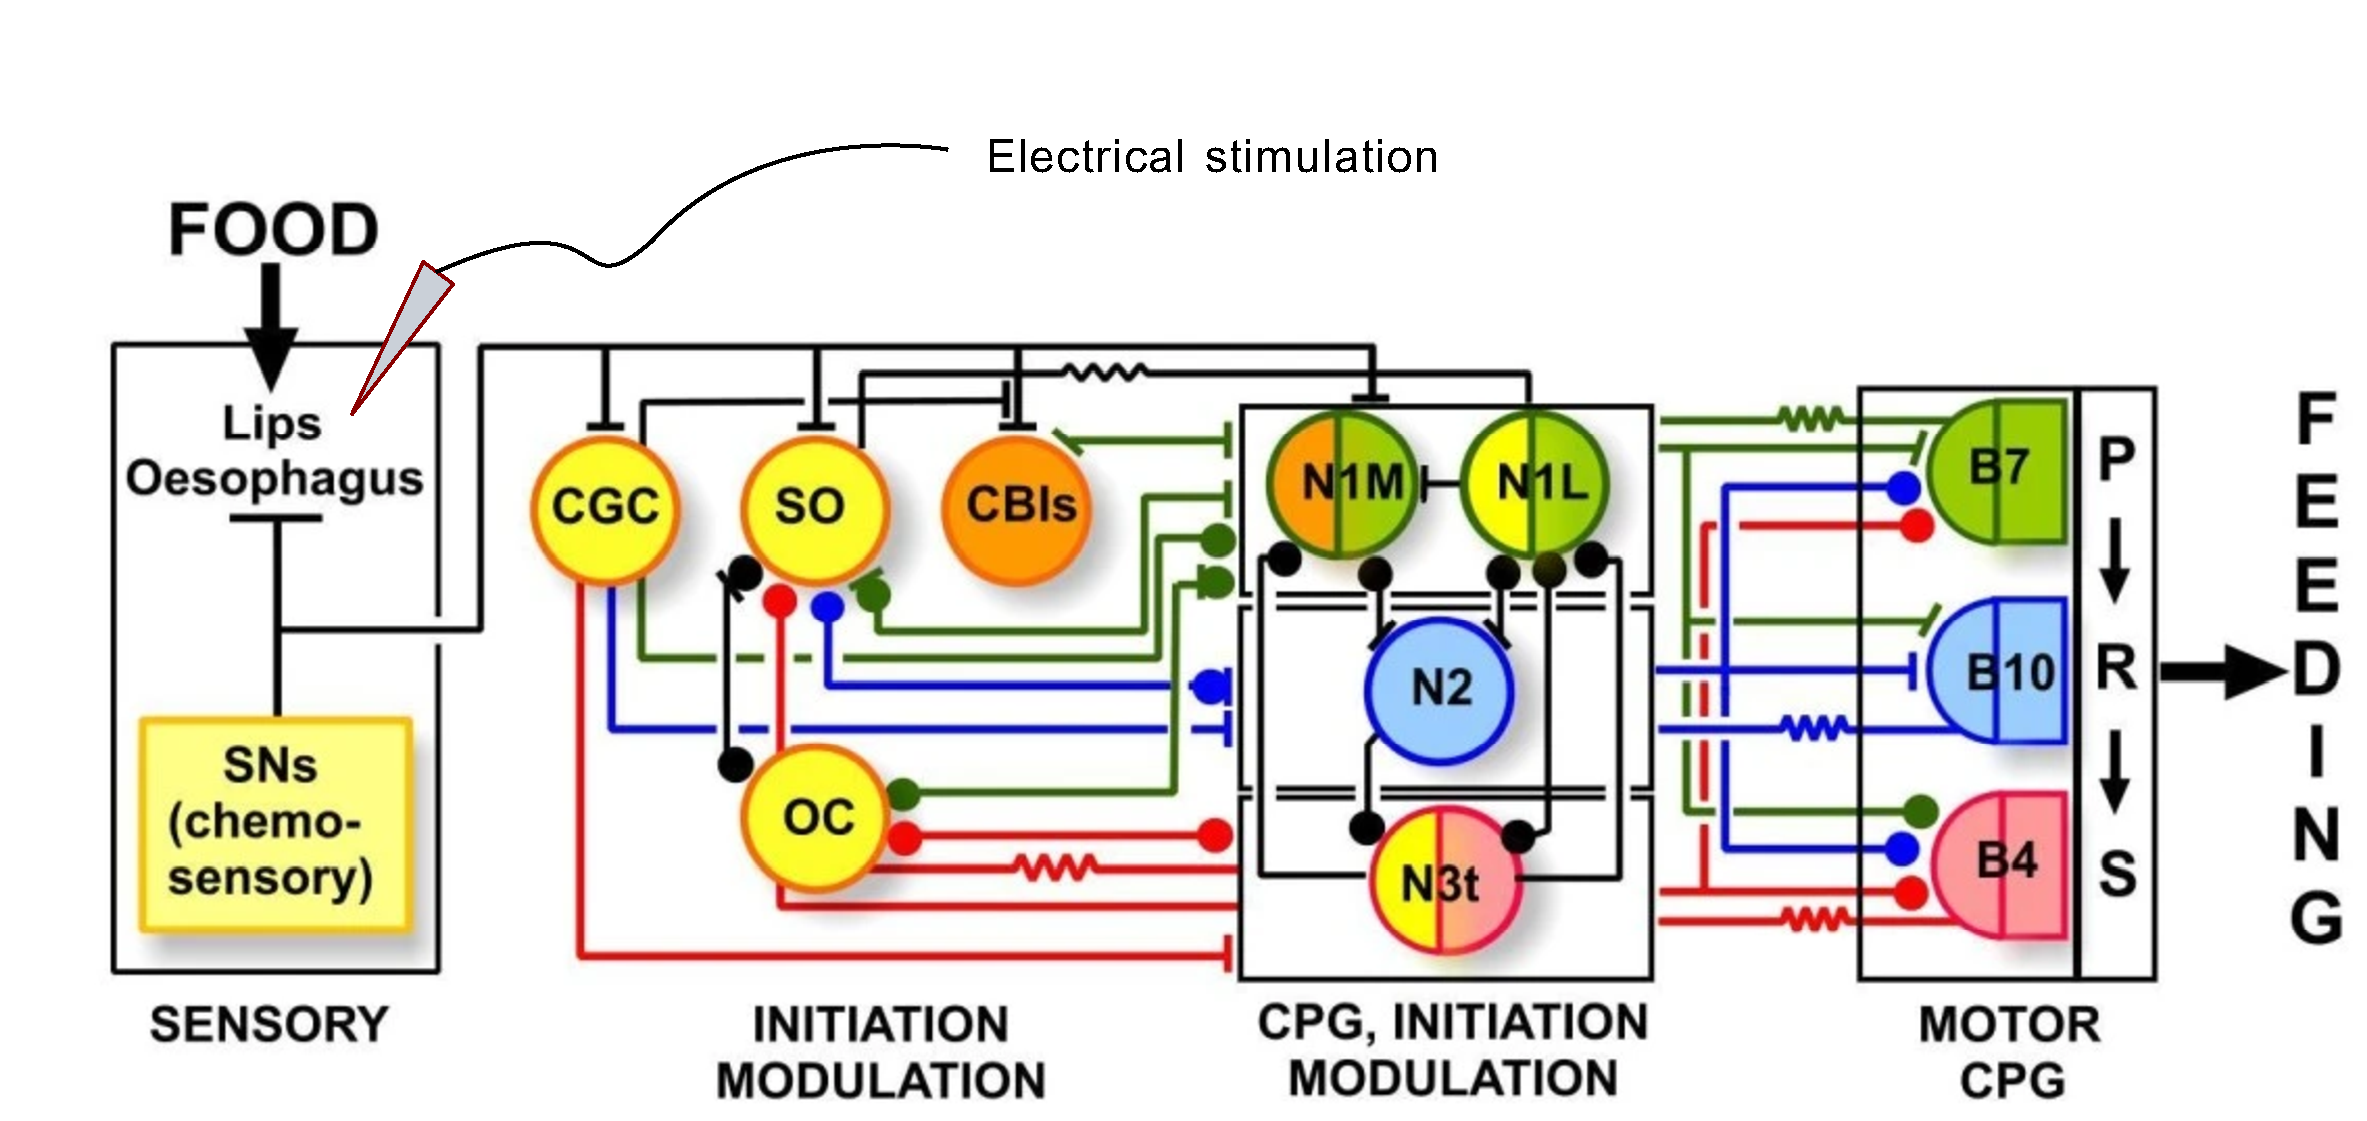
\includegraphics[width=\textwidth]{Images/distributed_benjamin_2012_electrophys_mln.pdf}
	\tiny{Benjamin, P. R. (2012). Distributed network organization underlying feeding behavior in the mollusk Lymnaea. Neural Systems \& Circuits, 2(1), 1–16. https://doi.org/10.1186/2042-1001-2-4}
	}
	\only<5>{
	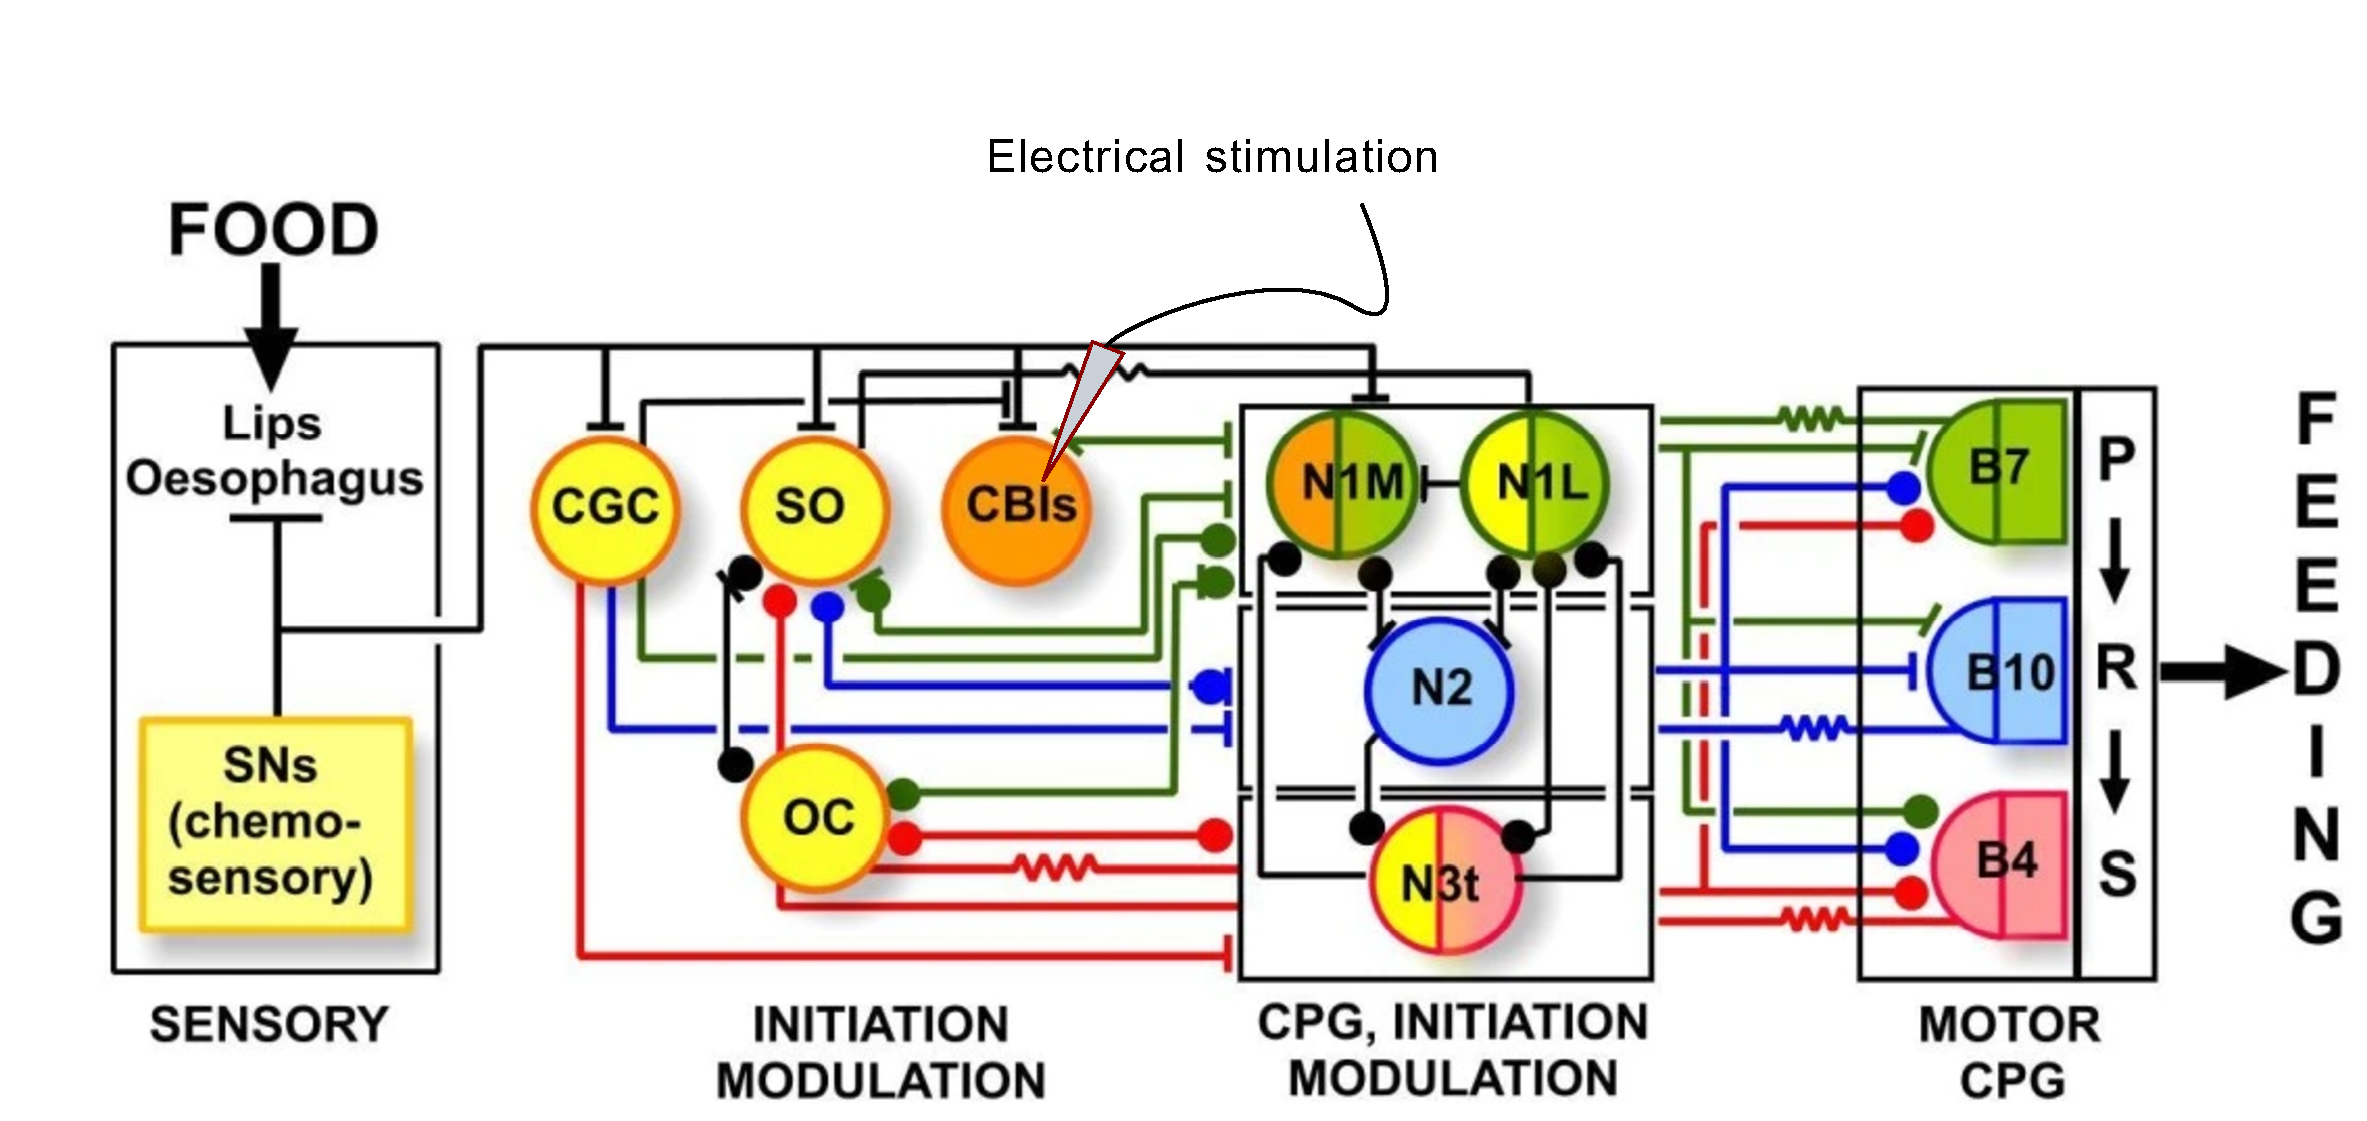
\includegraphics[width=\textwidth]{Images/distributed_benjamin_2012_electrophys_cv1a.pdf}
	\tiny{Benjamin, P. R. (2012). Distributed network organization underlying feeding behavior in the mollusk Lymnaea. Neural Systems \& Circuits, 2(1), 1–16. https://doi.org/10.1186/2042-1001-2-4}
	}

\end{frame}



\begin{frame}{Spontaneous activity}
	
	\only<1>{	
		\centering
		\begin{minipage}[c]{0.1\textwidth} % Adjust width for the label column
			\centering
			\rotatebox{90}{\small{Case 1}}
		\end{minipage}%
		\begin{minipage}[c]{0.85\textwidth}
			\centering
			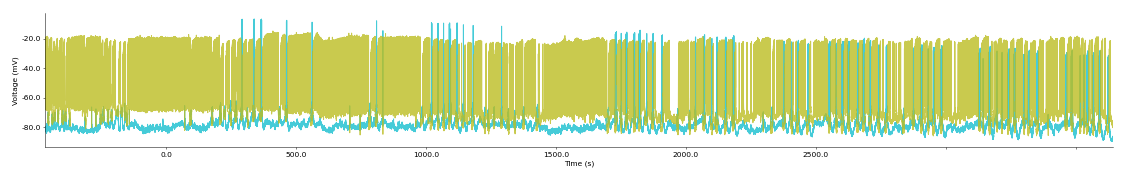
\includegraphics[width=\textwidth]{invariants/data/SUSSEX//prep2/images/3phases/_signal_intervals_zoom.png}\\
			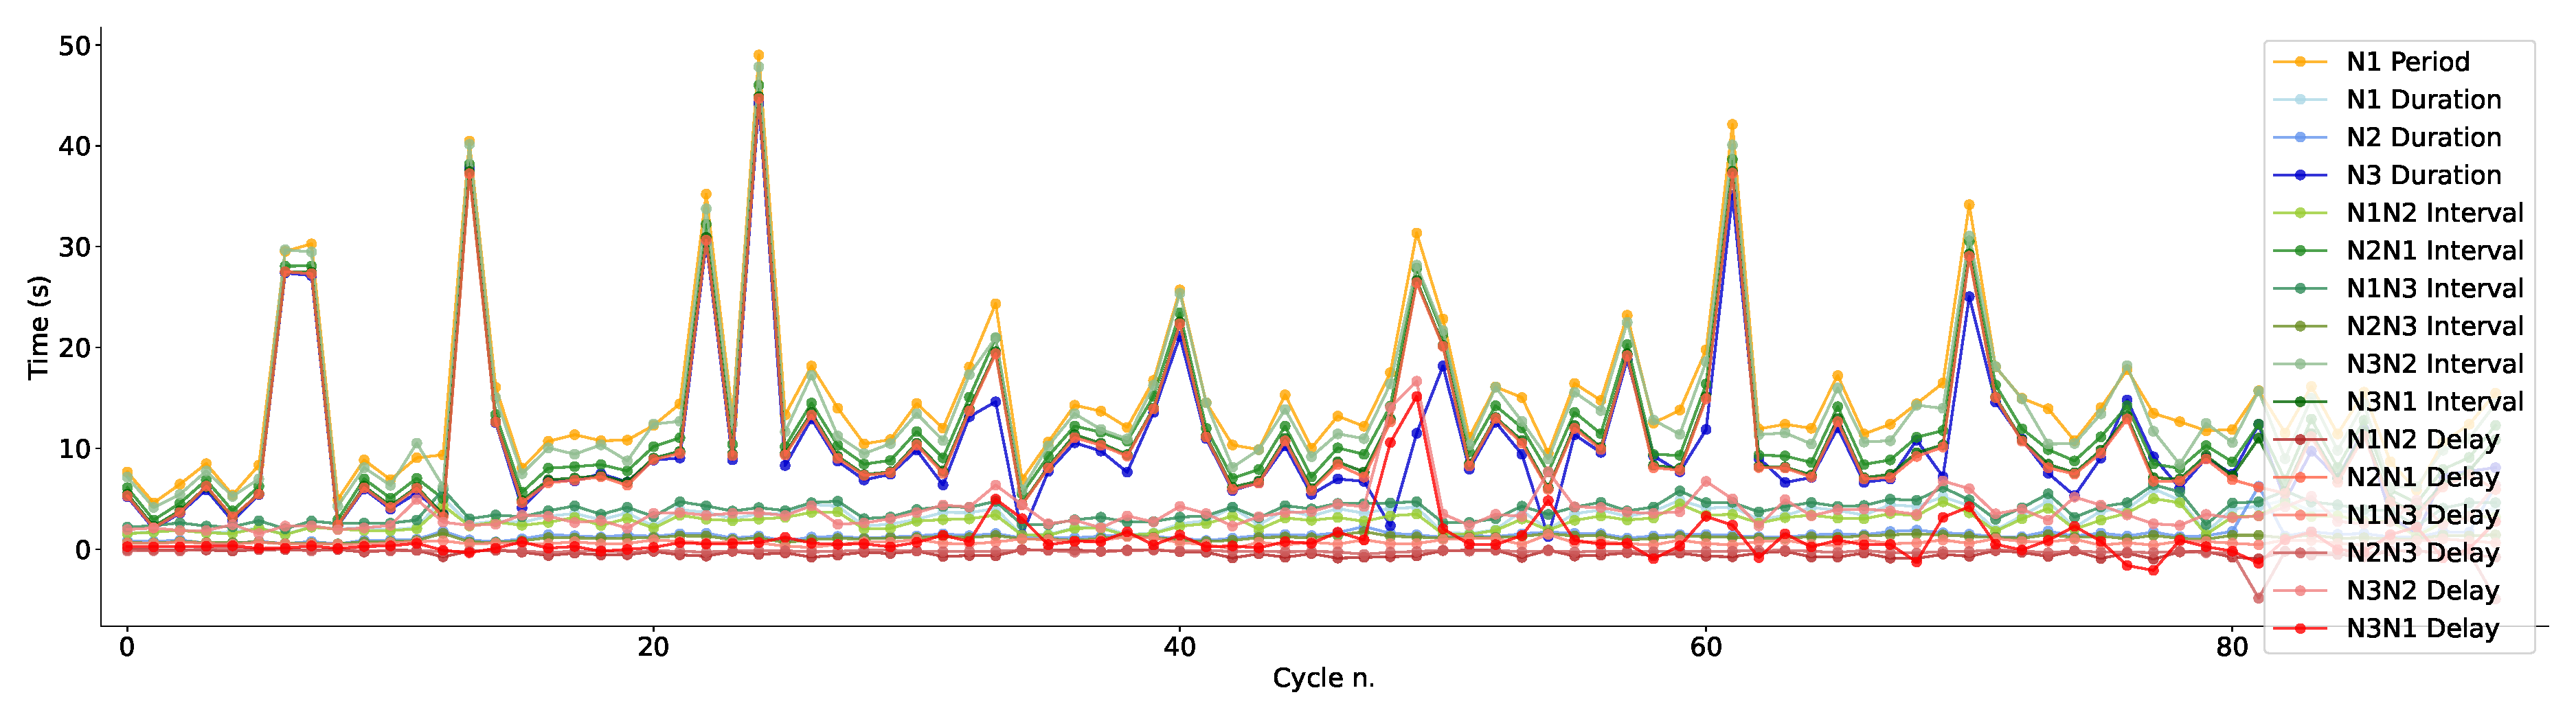
\includegraphics[width=\textwidth]{invariants/data/SUSSEX/prep2/images/3phases/_time_cycle.pdf}
		\end{minipage}
		
%		\vspace{0.5cm} % Add some space between the image sets
		
		\begin{minipage}[c]{0.1\textwidth} % Adjust width for the label column
			\centering
			\rotatebox{90}{\small{Case 2}}
		\end{minipage}%
		\begin{minipage}[c]{0.85\textwidth}
			\centering
			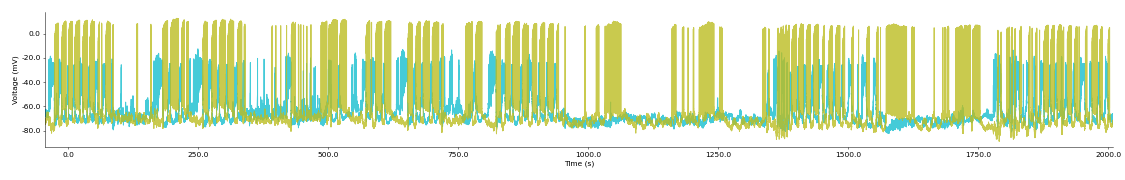
\includegraphics[width=\textwidth]{invariants/data/SUSSEX/prep3/images/3phases/_signal_intervals_zoom.png}\\
			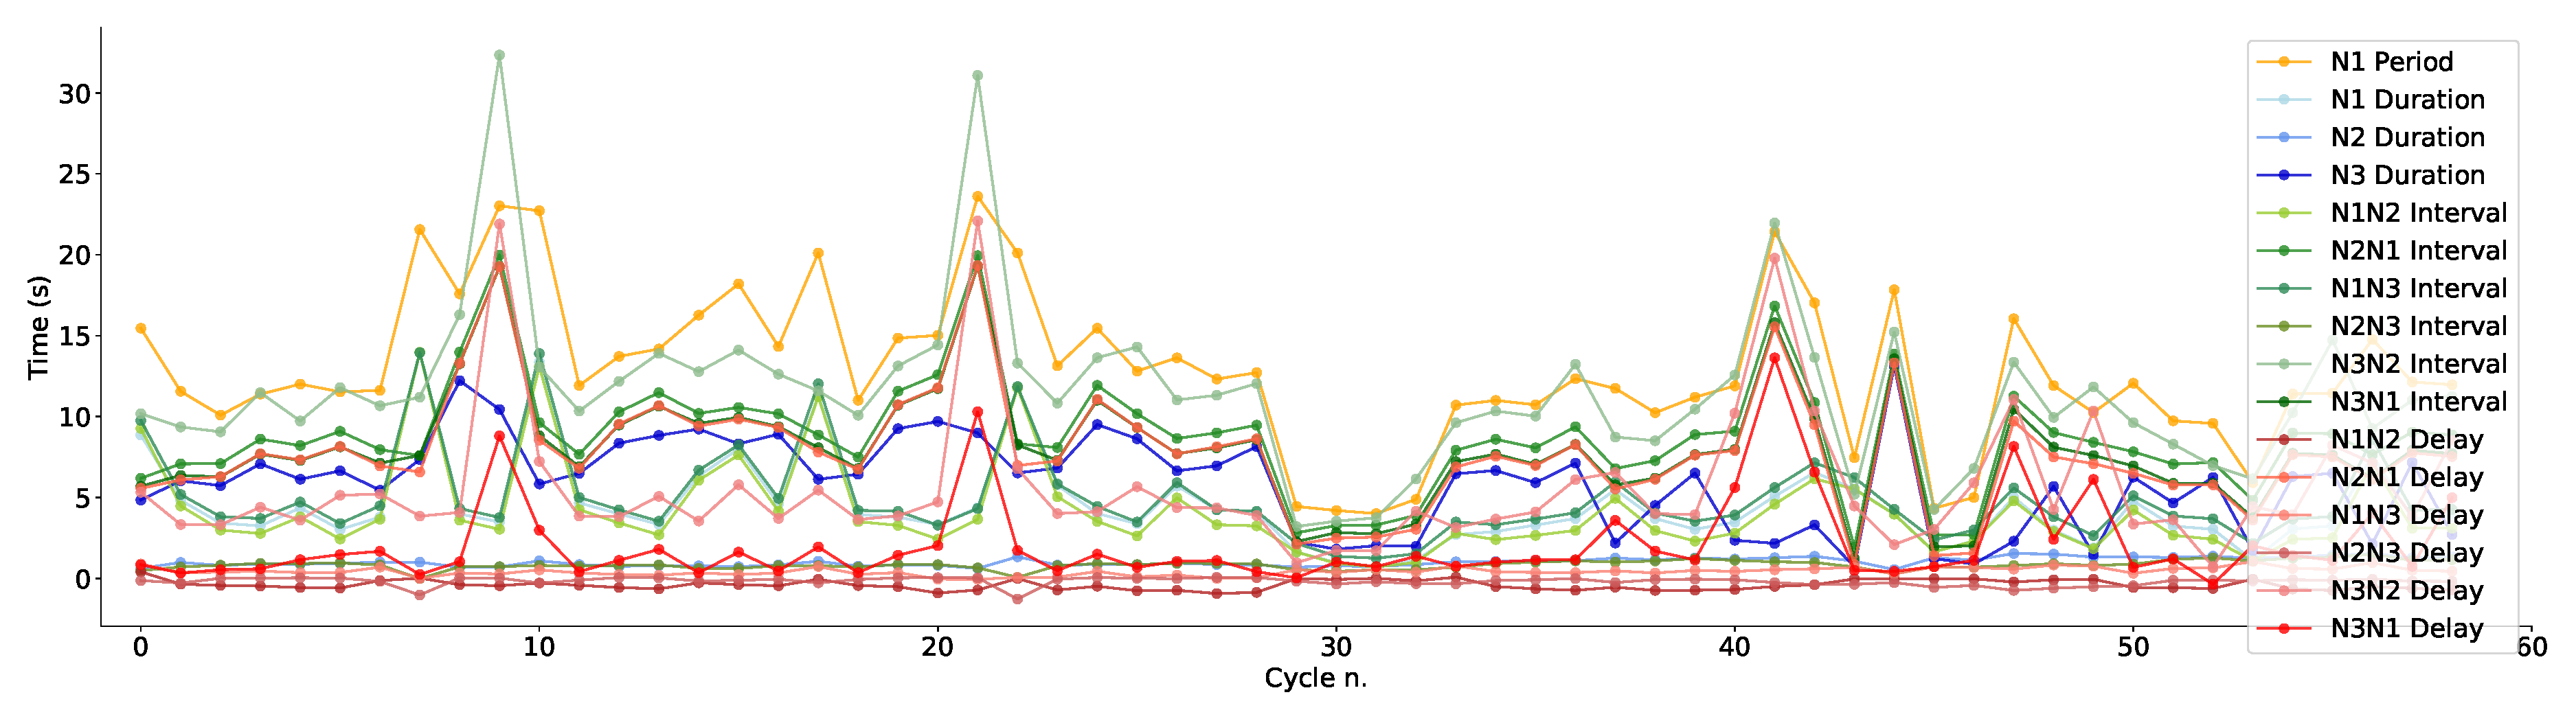
\includegraphics[width=\textwidth]{invariants/data/SUSSEX/prep3/images/3phases/_time_cycle.pdf}
		\end{minipage}
		
	}
	%%%%%%%%%%%%%%%%%%%%%%%%%%%%%%%%%%%%%%%%%
	%%%%% Boxplot
	%%%%%%%%%%%%%%%%%%%%%%%%%%%%%%%%%%%%%%%%%
%	\only<2>{
%		\centering \small{Case 1}				
%		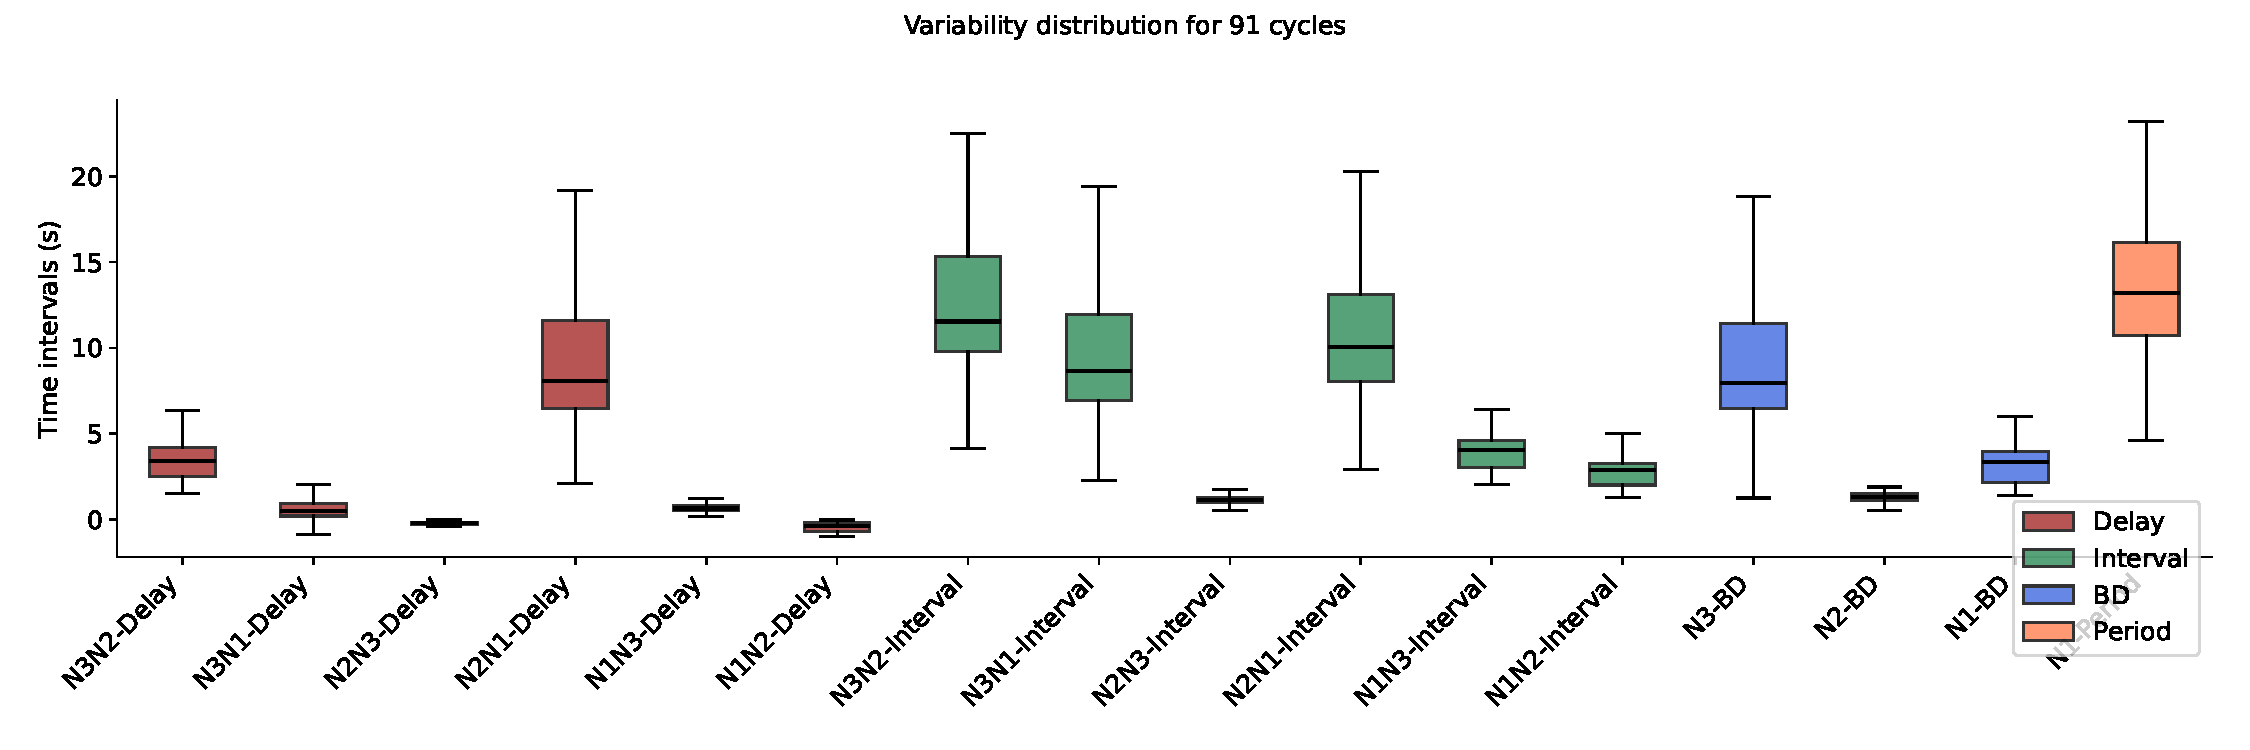
\includegraphics[width=\textwidth]{invariants/data/SUSSEX/prep2/images/3phases/_boxplot_h.pdf}
%
%		\centering \small{Case 2}
%		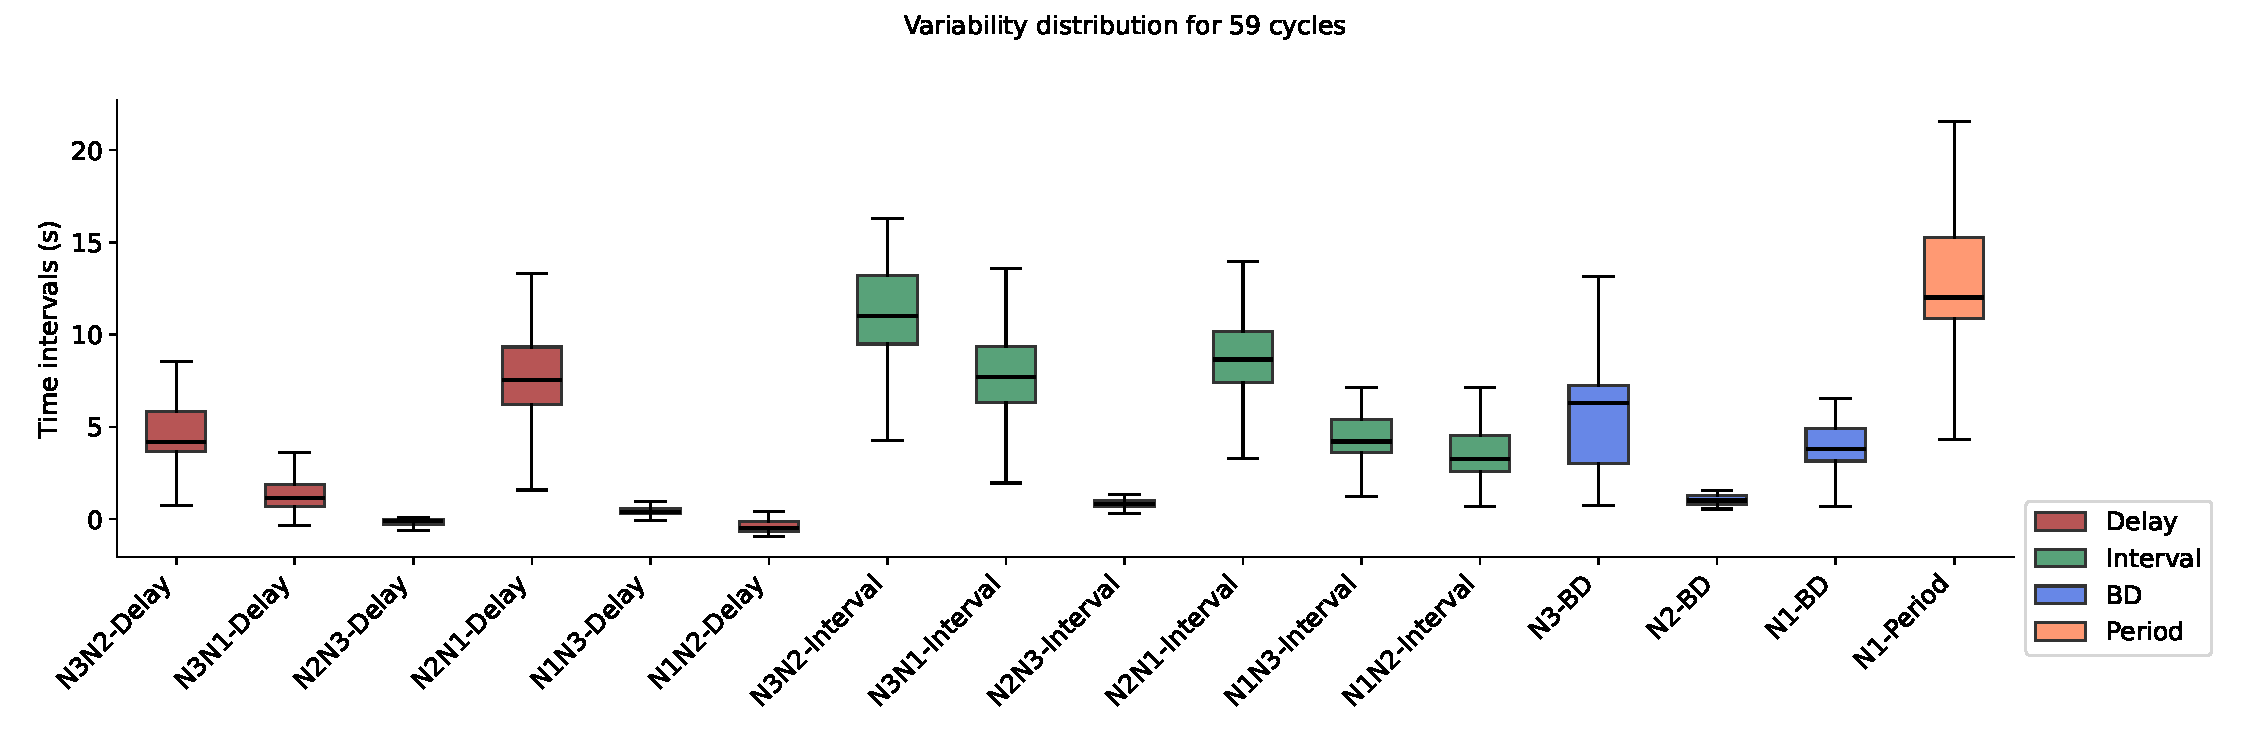
\includegraphics[width=\textwidth]{invariants/data/SUSSEX/prep3/images/3phases/_boxplot_h.pdf}
%
%	}

	%%%%%%%%%%%%%%%%%%%%%%%%%%%%%%%%%%%%%%%%%
	%%%%% Correlations
	%%%%%%%%%%%%%%%%%%%%%%%%%%%%%%%%%%%%%%%%%
	\only<2>{
		\begin{columns}
			\begin{column}{0.5\textwidth}
				\centering \small{Case 1\\}	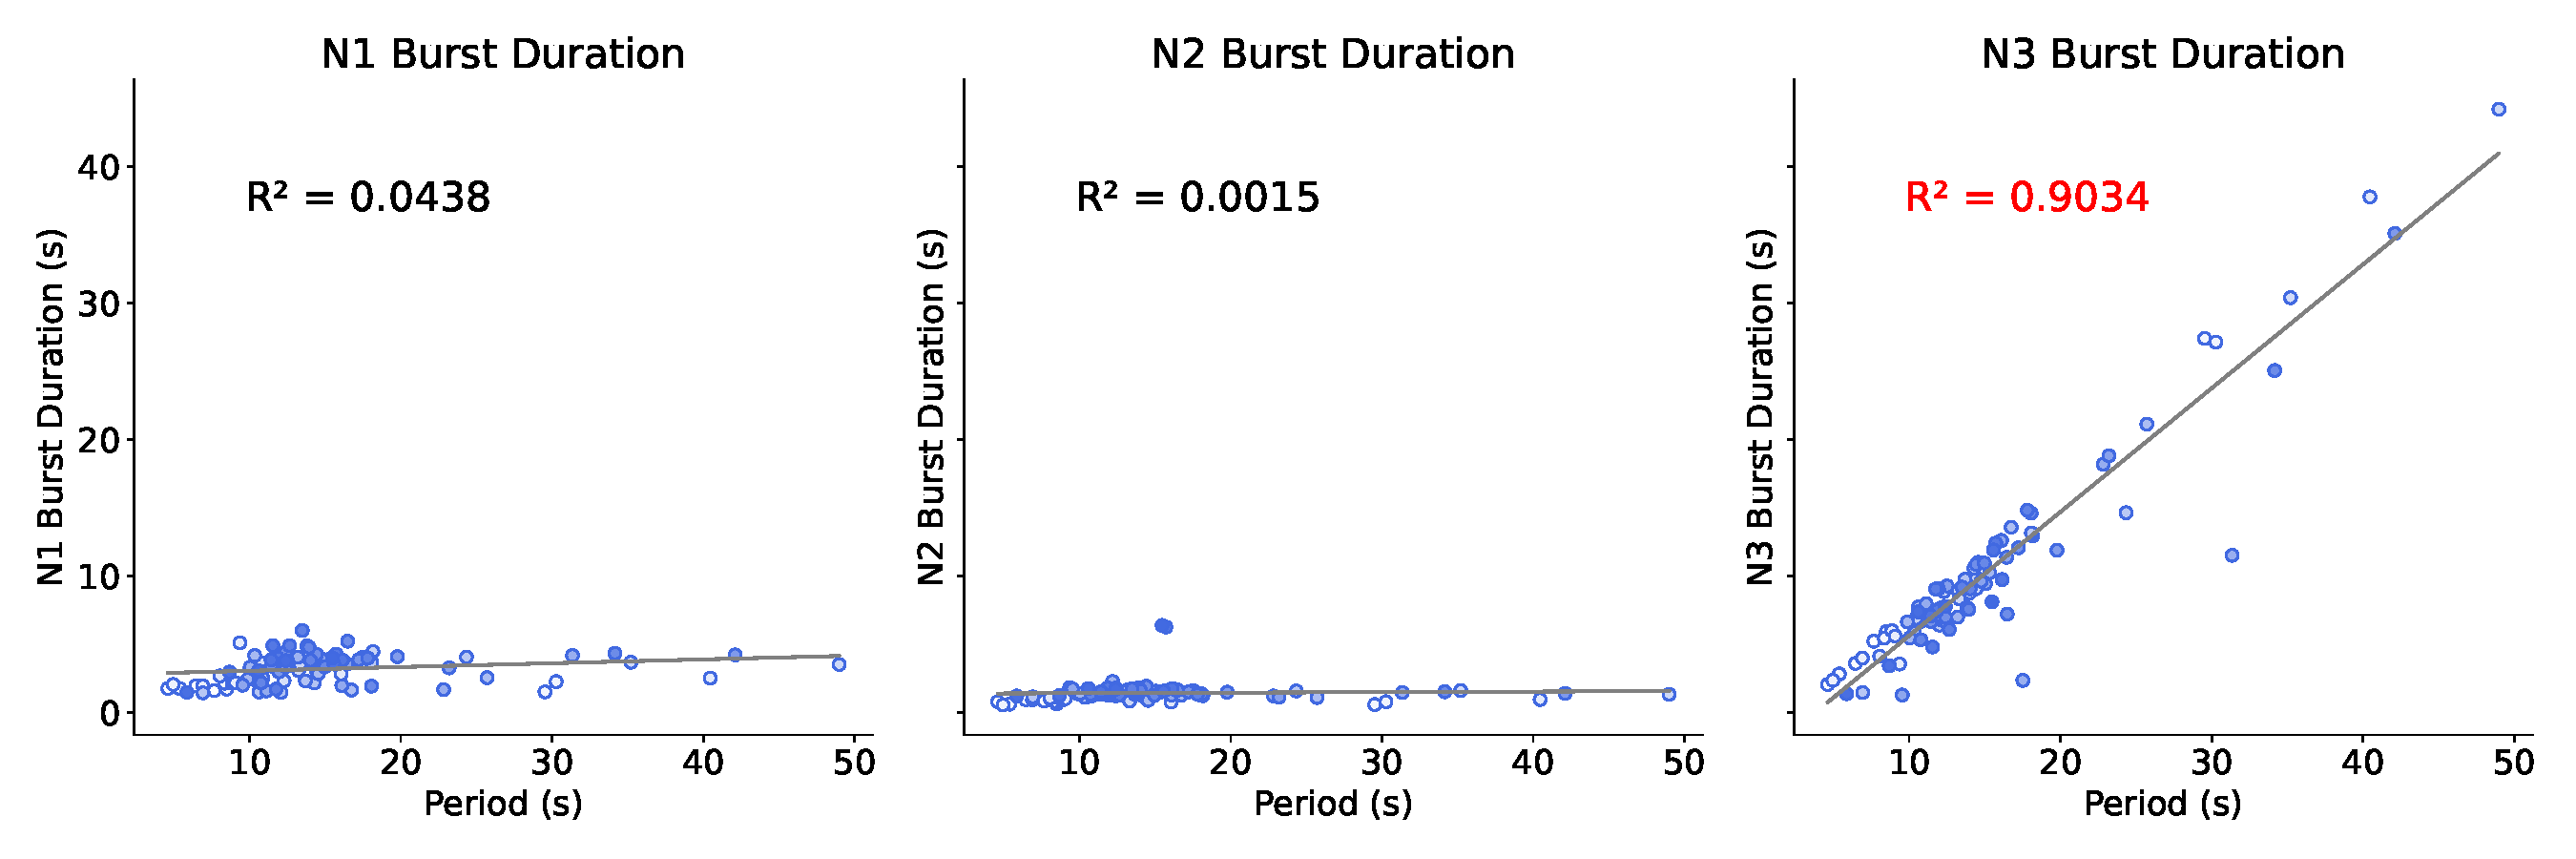
\includegraphics[width=0.85\textwidth]{invariants/data/SUSSEX/prep2/images/3phases/_durations.pdf}	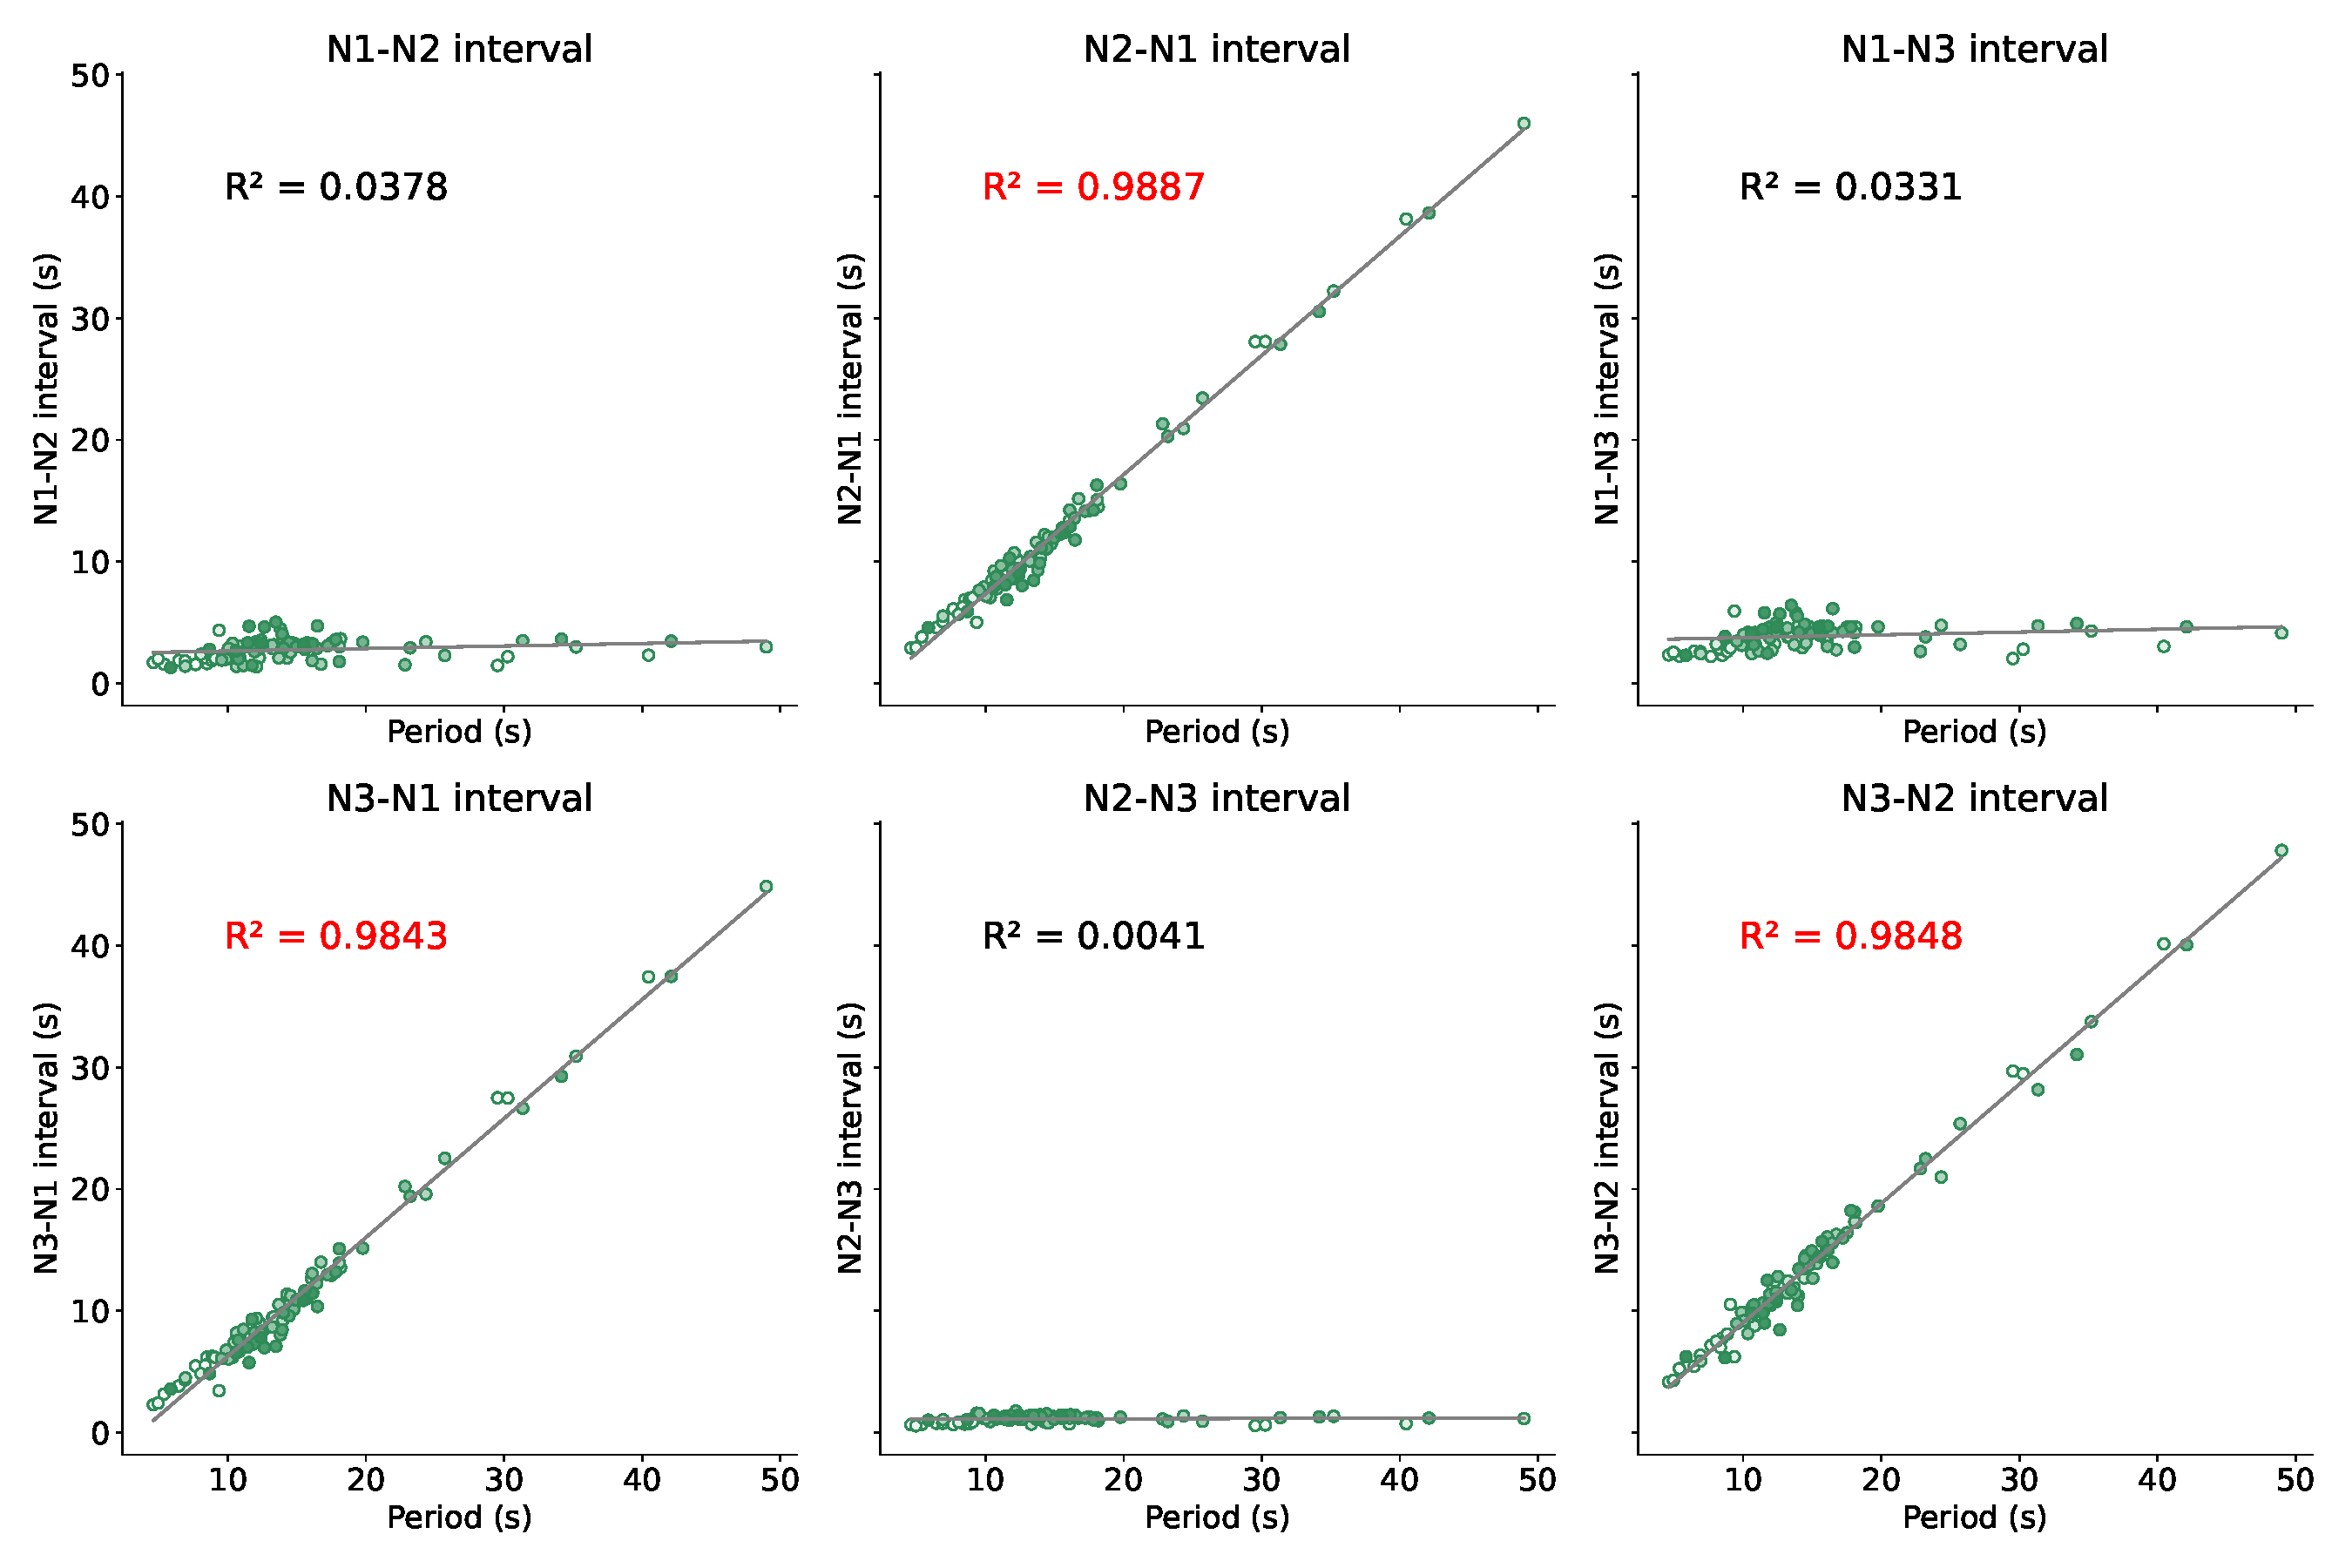
\includegraphics[width=0.9\textwidth]{invariants/data/SUSSEX/prep2/images/3phases/_intervals.pdf}	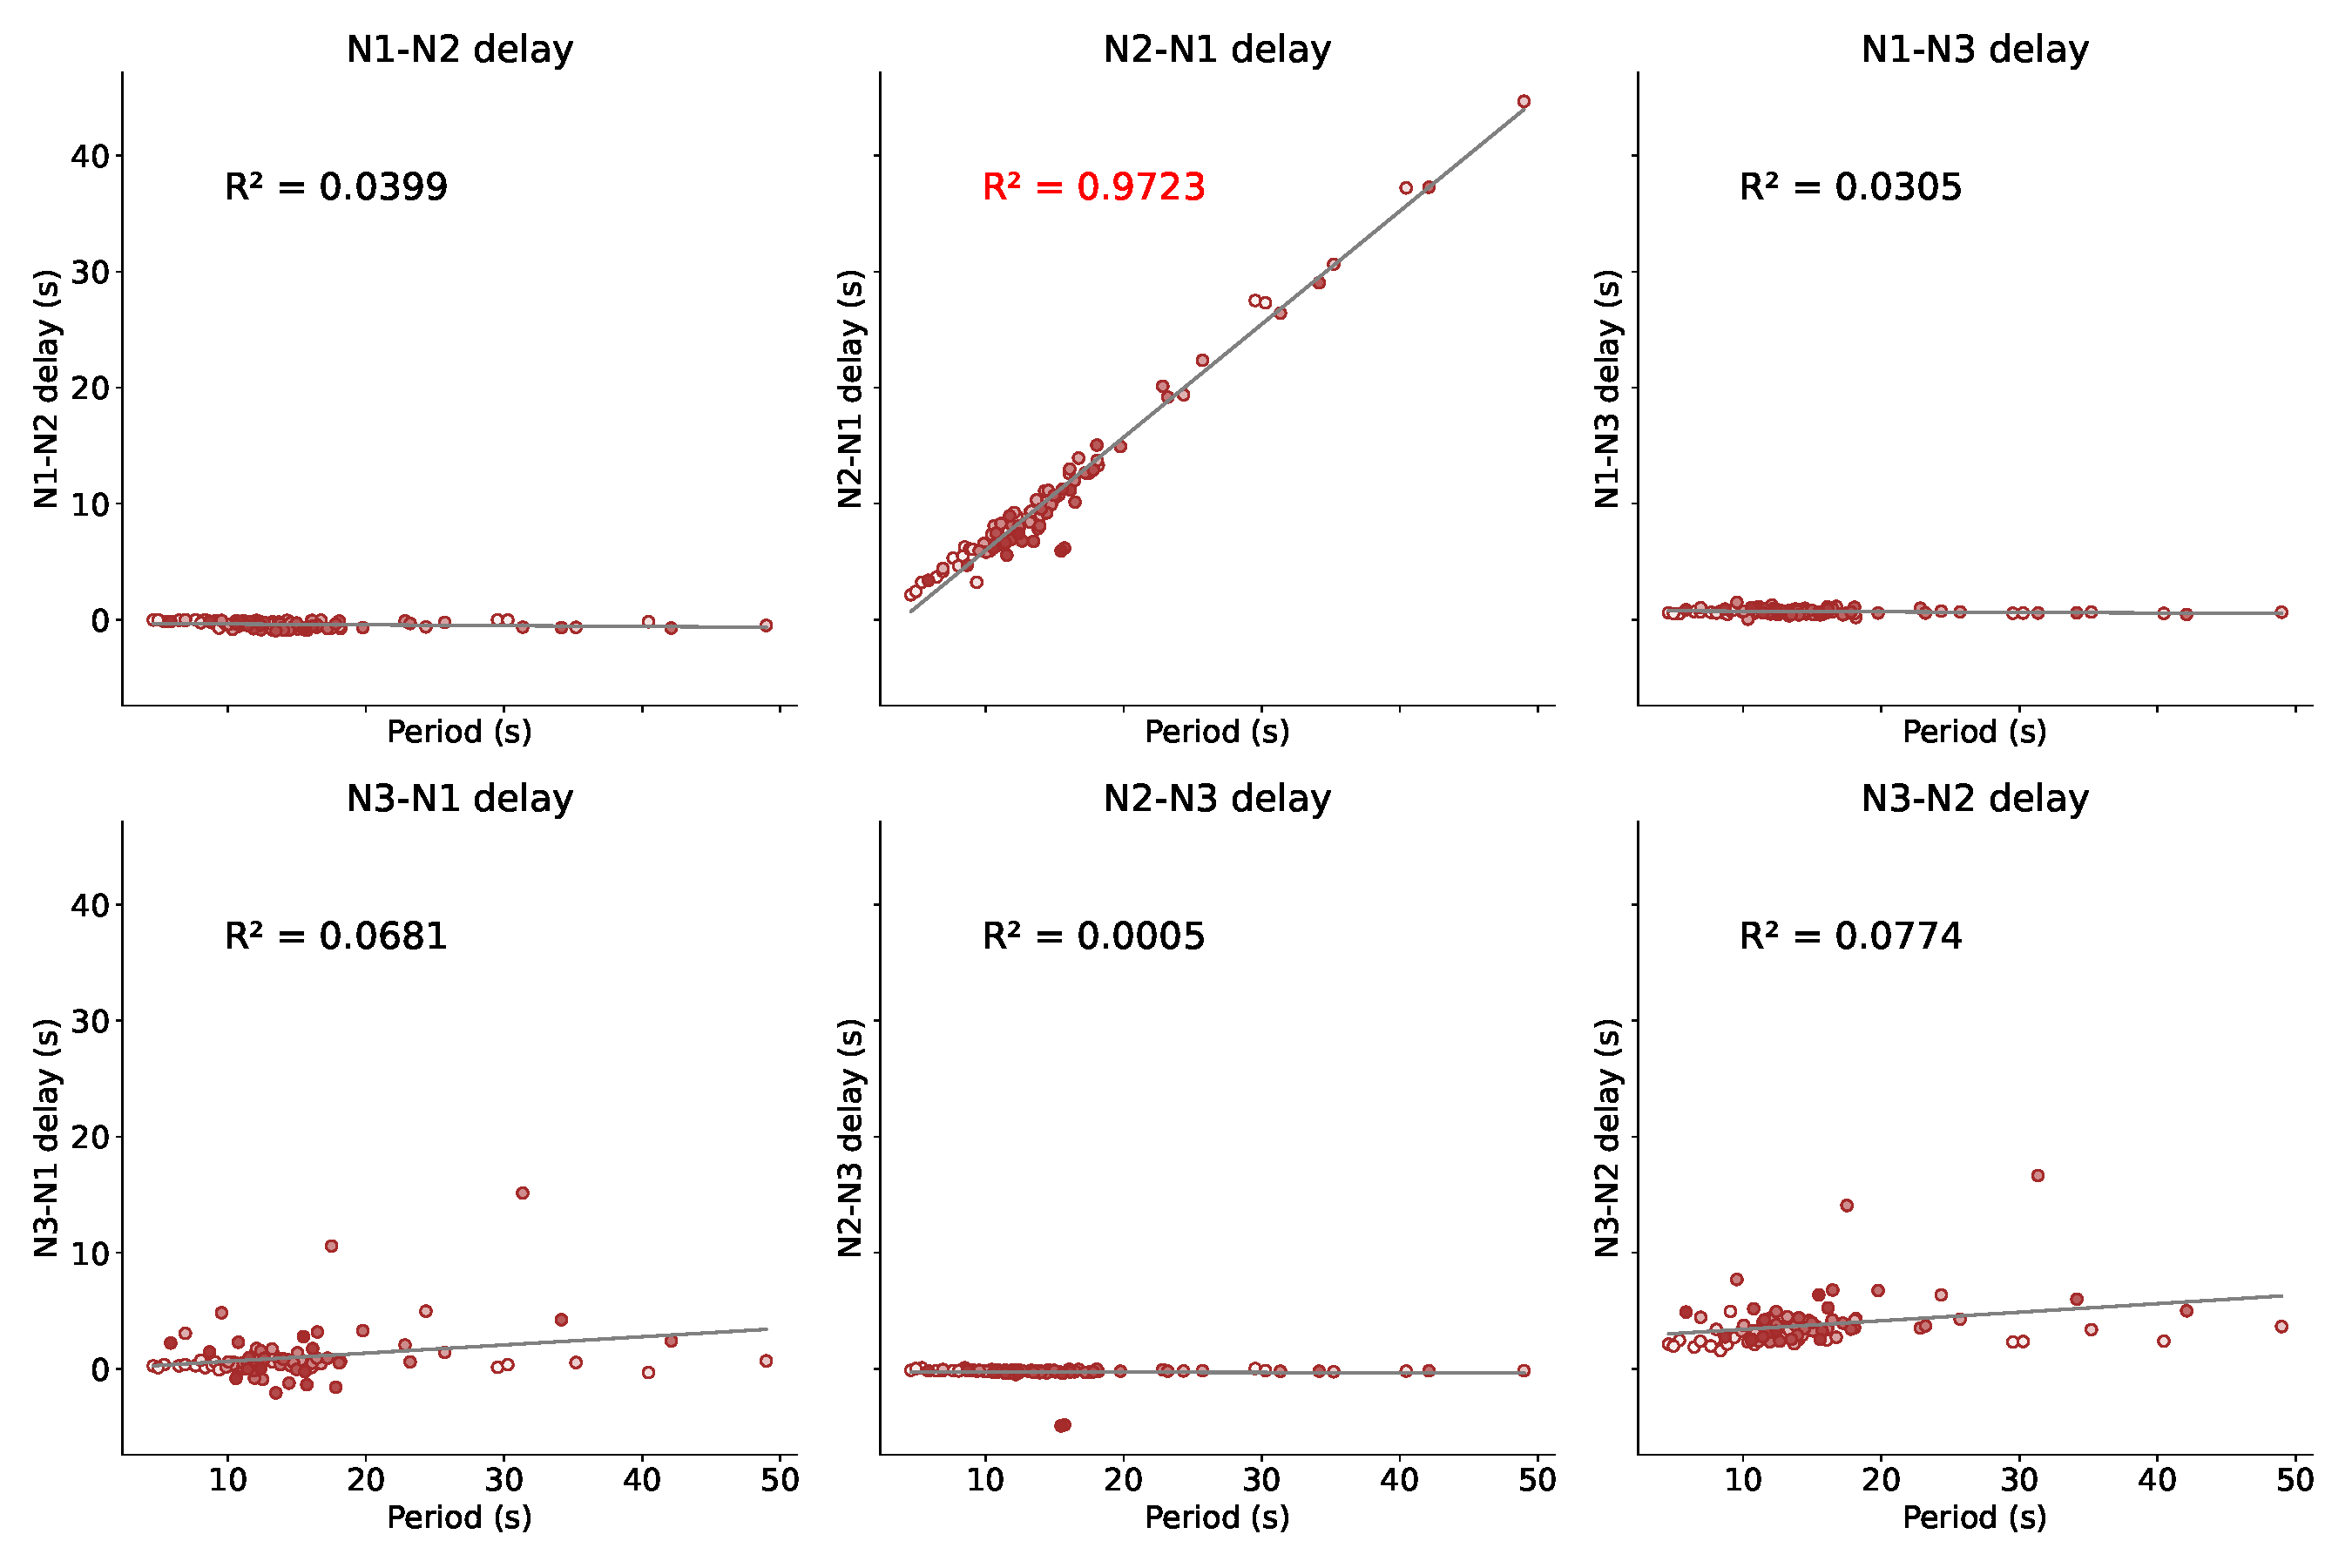
\includegraphics[width=0.9\textwidth]{invariants/data/SUSSEX/prep2/images/3phases/_delays.pdf}
				%				\includegraphics[width=\textwidth]{invariants/data/SUSSEX/prep2/images/3phases/panel_with_intervals_boxplot_invariants.pdf}
			\end{column}
			\begin{column}{0.5\textwidth}
				\centering \small{Case 2\\}	\includegraphics[width=0.85\textwidth]{invariants/data/SUSSEX/prep3/images/3phases/_durations.pdf}	\includegraphics[width=0.9\textwidth]{invariants/data/SUSSEX/prep3/images/3phases/_intervals.pdf}	\includegraphics[width=0.9\textwidth]{invariants/data/SUSSEX/prep3/images/3phases/_delays.pdf}
	%			\centering Case 2
	%			\includegraphics[width=\textwidth]{invariants/data/SUSSEX/prep3/images/3phases/panel_with_intervals_boxplot_invariants.pdf}
			\end{column}
		\end{columns}
	}
%TODO arregar, poner etiquetas a ,b, c y que se vea todo
\end{frame}


\begin{frame}{SO driven activity}
\only<1>{	
		\centering
		\begin{minipage}[c]{0.1\textwidth} % Adjust width for the label column
			\centering
			\rotatebox{90}{\small{Induced SO driven}}
		\end{minipage}%
		\begin{minipage}[c]{0.85\textwidth}
			\centering
			\includegraphics[width=\textwidth]{invariants/data/SUSSEX/SO_driven/images/_signal_intervals_zoom.png}\\
			\includegraphics[width=\textwidth]{invariants/data/SUSSEX/SO_driven/images/_time_cycle.pdf}
		\end{minipage}
		
%		\vspace{0.5cm} % Add some space between the image sets
		
		\begin{minipage}[c]{0.1\textwidth} % Adjust width for the label column
			\centering
			\rotatebox{90}{\small{Spontaneous SO driven}}
		\end{minipage}%
		\begin{minipage}[c]{0.85\textwidth}
			\centering
			\includegraphics[width=\textwidth]{invariants/data/SUSSEX/prep4_so_driven_2/images/_signal_intervals_zoom.png}\\
			\includegraphics[width=\textwidth]{invariants/data/SUSSEX/prep4_so_driven_2/images/_time_cycle.pdf}
		\end{minipage}

}
\only<2>{
	\begin{columns}
		\begin{column}{0.5\textwidth}
%			\centering \small{SO driven by stimulation}
%			\includegraphics[width=\textwidth]{invariants/data/SUSSEX/SO_driven/images/panel_with_intervals_boxplot_invariants.pdf}
			\includegraphics[width=\textwidth]{invariants/data/SUSSEX/SO_driven/images/_boxplot_h.pdf}
			\centering
				\includegraphics[width=0.8\textwidth]{invariants/data/SUSSEX/SO_driven/images/_durations.pdf}	\includegraphics[width=0.8\textwidth]{invariants/data/SUSSEX/SO_driven/images/_intervals.pdf}	\includegraphics[width=0.8\textwidth]{invariants/data/SUSSEX/SO_driven/images/_delays.pdf}
		\end{column}
		\begin{column}{0.5\textwidth}
%			\centering \small{SO spontaneous driven}
%		\includegraphics[width=\textwidth]{invariants/data/SUSSEX/prep4_so_driven_2/images/panel_with_intervals_boxplot_invariants.pdf}
			\includegraphics[width=\textwidth]{invariants/data/SUSSEX/prep4_so_driven_2/images/_boxplot_h.pdf}
			\centering
				\includegraphics[width=0.8\textwidth]{invariants/data/SUSSEX/prep4_so_driven_2/images/_durations.pdf}	\includegraphics[width=0.8\textwidth]{invariants/data/SUSSEX/prep4_so_driven_2/images/_intervals.pdf}	\includegraphics[width=0.8\textwidth]{invariants/data/SUSSEX/prep4_so_driven_2/images/_delays.pdf}	
			
%			\includegraphics[width=\textwidth]{invariants/data/SUSSEX/prep4_so_driven_2/images/panel_with_intervals_boxplot_invariants.pdf}
%			\includegraphics[width=\textwidth]{invariants/data/SUSSEX/prep4_so_driven_2/images/panel_with_intervals_boxplot_invariants.pdf}
		\end{column}
	\end{columns}
}	
%TODO poner Diagrama en pequeñito para referencia

\end{frame}



%\begin{frame}{MLN driven activity}
%	\begin{columns}
%		\uncover<1->{
%			\begin{column}{0.58\textwidth}
%				\includegraphics[width=\textwidth]{invariants/data/SUSSEX/MLN_driven/images/panel_variability_zoom.pdf}
%			\end{column}
%		}
%		\uncover<2>{
%			\begin{column}{0.5\textwidth}
%				\includegraphics[width=\textwidth]{invariants/data/SUSSEX/MLN_driven/images/panel_with_intervals_boxplot_invariants.pdf}
%			\end{column}
%		}
%	\end{columns}
%%TODO poner Diagrama en pequeñito para referencia
%\end{frame}


\begin{frame}{MLN driven activity}
	\begin{columns}
		\uncover<1->{
			\begin{column}{0.7\textwidth}
				\includegraphics[width=\textwidth]{invariants/data/SUSSEX/MLN_driven/images/_signal_intervals_zoom.png}
				\includegraphics[width=\textwidth]{invariants/data/SUSSEX/MLN_driven/images/_signal_intervals_cycle.pdf}
				\includegraphics[width=\textwidth]{invariants/data/SUSSEX/MLN_driven/images/_time_cycle.pdf}
				\includegraphics[width=\textwidth]{invariants/data/SUSSEX/MLN_driven/images/_boxplot_h.pdf}
			\end{column}
		}
		\uncover<2>{
			\begin{column}{0.4\textwidth}
				\includegraphics[width=\textwidth]{invariants/data/SUSSEX/MLN_driven/images/_durations.pdf}	\includegraphics[width=\textwidth]{invariants/data/SUSSEX/MLN_driven/images/_intervals.pdf}	\includegraphics[width=\textwidth]{invariants/data/SUSSEX/MLN_driven/images/_delays.pdf}
			\end{column}
		}
	\end{columns}
	%TODO poner Diagrama en pequeñito para referencia
\end{frame}



\begin{frame}{CV1a driven activity}
	\only<1>{	
		\centering
		\begin{minipage}[c]{0.1\textwidth} % Adjust width for the label column
			\centering
			\rotatebox{90}{\small{CV1a driven (1)}}
		\end{minipage}%
		\begin{minipage}[c]{0.85\textwidth}
			\centering
			\includegraphics[width=\textwidth]{invariants/data/SUSSEX/CV1a_driven1/images/2phases/_signal_intervals_zoom.png}\\
			\includegraphics[width=\textwidth]{invariants/data/SUSSEX/CV1a_driven1/images/2phases/_time_cycle.pdf}
		\end{minipage}
		
		%		\vspace{0.5cm} % Add some space between the image sets
		
		\begin{minipage}[c]{0.1\textwidth} % Adjust width for the label column
			\centering
			\rotatebox{90}{\small{CV1a driven (2)}}
		\end{minipage}%
		\begin{minipage}[c]{0.85\textwidth}
			\centering
			\includegraphics[width=\textwidth]{invariants/data/SUSSEX/CV1a_driven2/images/_signal_intervals_zoom.png}\\
			\includegraphics[width=\textwidth]{invariants/data/SUSSEX/CV1a_driven2/images/_time_cycle.pdf}
		\end{minipage}
		
	}
	\only<2>{
		\begin{columns}
			\begin{column}{0.5\textwidth}
				%			\centering \small{CV1a driven (1)}
				%			\includegraphics[width=\textwidth]{invariants/data/SUSSEX/SO_driven/images/panel_with_intervals_boxplot_invariants.pdf}
				\includegraphics[width=\textwidth]{invariants/data/SUSSEX/CV1a_driven1/images/2phases/_boxplot_h.pdf}
				\centering
				\includegraphics[width=0.8\textwidth]{invariants/data/SUSSEX/CV1a_driven1/images/2phases/_durations.pdf}	\includegraphics[width=0.8\textwidth]{invariants/data/SUSSEX/CV1a_driven1/images/2phases/_intervals.pdf}	\includegraphics[width=0.8\textwidth]{invariants/data/SUSSEX/CV1a_driven1/images/2phases/_delays.pdf}
			\end{column}
			\begin{column}{0.5\textwidth}
				%			\centering \small{CV1a driven (2)}
				%		\includegraphics[width=\textwidth]{invariants/data/SUSSEX/prep4_so_driven_2/images/panel_with_intervals_boxplot_invariants.pdf}
				\includegraphics[width=\textwidth]{invariants/data/SUSSEX/CV1a_driven2/images/_boxplot_h.pdf}
				\centering
				\includegraphics[width=0.8\textwidth]{invariants/data/SUSSEX/CV1a_driven2/images/_durations.pdf}	\includegraphics[width=0.8\textwidth]{invariants/data/SUSSEX/CV1a_driven2/images/_intervals.pdf}	\includegraphics[width=0.8\textwidth]{invariants/data/SUSSEX/CV1a_driven2/images/_delays.pdf}	
				
				%			\includegraphics[width=\textwidth]{invariants/data/SUSSEX/prep4_so_driven_2/images/panel_with_intervals_boxplot_invariants.pdf}
				%			\includegraphics[width=\textwidth]{invariants/data/SUSSEX/prep4_so_driven_2/images/panel_with_intervals_boxplot_invariants.pdf}
			\end{column}
		\end{columns}
	}	
	%TODO poner Diagrama en pequeñito para referencia
	
\end{frame}
%
%\begin{frame}{CV1 driven activity}
%	\only<1>{	
%		\begin{columns}
%			\begin{column}{0.57\textwidth}
%				\centering CV1a driven by electrical stimulation. Case 1
%				\includegraphics[width=\textwidth]{invariants/data/SUSSEX/CV1a_driven1/images/2phases/panel_variability_zoom.pdf}
%			\end{column}
%			\begin{column}{0.57\textwidth}
%				\centering CV1a driven by electrical stimulation. Case 2
%				\includegraphics[width=\textwidth]{invariants/data/SUSSEX/CV1a_driven2/images/panel_variability_zoom.pdf}
%			\end{column}
%		\end{columns}
%	}
%	\only<2>{
%		\begin{columns}
%			\begin{column}{0.5\textwidth}
%				\centering CV1a driven by electrical stimulation. Case 1
%				\includegraphics[width=\textwidth]{invariants/data/SUSSEX/CV1a_driven1/images/2phases/panel_with_intervals_boxplot_invariants.pdf}
%			\end{column}
%			\begin{column}{0.5\textwidth}
%				\centering CV1a driven by electrical stimulation. Case 2
%				\includegraphics[width=\textwidth]{invariants/data/SUSSEX/CV1a_driven2/images/panel_with_intervals_boxplot_invariants.pdf}
%			\end{column}
%		\end{columns}
%	}
%%TODO poner Diagrama en pequeñito para referencia
%\end{frame}

\begin{frame}{Study of functional the role of dynamical invariants in a Hybrot}
\only<1>{
\centering
\movie[label=Robot,width=\textwidth,poster=false,autostart=false,showcontrols,loop] 
{\includegraphics[width=\textwidth]{invariants/robot/Figure1_experiment_design_v1.png}}{Movies/GNB Hybrot with living CPG.mp4}
}
\only<2>{\centering\includegraphics[width=\textwidth]{invariants/robot/robot_results_invariant.png}}
\note{Solución de inteniería, 'mas biologico'´} 
\end{frame}


\begin{frame}{Summary of results}
	\centering
	\includegraphics[width=0.95\textwidth]{Images/invariants_summary.png}
\end{frame}


\section[CW-NIR Neuromodulation]{CW-NIR laser stimulation as an effective neuromodulation technique}
\note{MOTIVATE "STUDY OF SEQUENCES WITH LASER STIMULATION"}
\begin{frame}{Current findings}
	\begin{itemize}
		\item{Laser stimulation accelerates neural activity.}
		\item{Most studies use pulsed laser and general dynamics} \note{Por qué pulsado y pq aqui no}
		\item{Open questions:}
		\begin{itemize}
			\item Source of the effect: Photothermal, Photomechanical ...
			\item Biophysical candidates: Capacitance, TRPV-4 
		\end{itemize}
	\end{itemize}
	\vspace{10pt}
	\begin{columns}
		\begin{column}{0.5\textwidth}
			\centering
			Clinical applications\\
			\includegraphics[width=0.8\textwidth]{Images/saucedo.png} \tiny{Figure 2 from Saucedo, C. L.et al (2021). Brain Stimulation, 14(2), 440–449. https://doi.org/10.1016/j.brs.2021.02.011}
		\end{column}
		\begin{column}{0.5\textwidth}
			\centering
			Stimulation technique\\
			\includegraphics[width=\textwidth]{Images/liang.png} \tiny{Figure 6A from Liang, S.et al. (2009). Cell Biochemistry and Biophysics, 53(1), 33–42. https://doi.org/10.1007/s12013-008-9035-2
			}
		\end{column}	
	\end{columns}
	
	
\end{frame}
\begin{frame}{Experimental setup}
	\centering
	\includegraphics[width=0.8\textwidth]{methods/laser-setup_labels.png}
\end{frame}

\begin{frame}{Sustained stimulation protocol}
	\begin{columns}
		\begin{column}{0.65\textwidth}
			\begin{itemize}
				\item {The neuron was illuminated during the intracellular recording.}
				\item {The illumination lasted 1-3 min.}
				\item {We recorded a control before and after the illumination.}
			\end{itemize}
		\end{column}
		\begin{column}{0.35\textwidth}
			\includegraphics[width=\textwidth]{laser/laser-beam.pdf}
		\end{column}
	\end{columns} 
	\vspace{15pt}
	\centering
	\includegraphics[width=0.8\textwidth]{laser/trial-protocol.pdf}
\end{frame}

\begin{frame}{Spike Waveform Characterization}
	\centering
	To characterize the change in the spike dynamics we defined waveform metrics. \\
	\vspace{15pt}
	\includegraphics[width=\textwidth]{laser/spike_metrics.pdf}
\end{frame}

\begin{frame}{Modulation of the spike waveform}
	\includegraphics[width=\textwidth]{laser/Figure2.png}
\end{frame}

\begin{frame}{Effect on the firing rate}
	\centering
	\includegraphics[width=\textwidth]{laser/frequency-small.pdf}
	%TODO añadir título
\end{frame}


\begin{frame}{Effect on a minimal circuit}
	
	\begin{columns}
		\begin{column}{0.3\textwidth}
			\includegraphics[width=\textwidth]{Images/electrical_ganglia.png}
		\end{column}
	\vspace{15pt}
		\begin{column}{0.7\textwidth}
			The stimulation of electrically coupled neurons, showed a first approximation to the capacity of the laser illumination to modulate neural dynamics. 
		\end{column}
	\end{columns}
	\centering
	\includegraphics[width=0.8\textwidth]{Images/electrical_result.png}	
\end{frame}

%\begin{frame}{Biophysical candidates}
%		There are distinct candidates under discussion
%		\begin{itemize}
%			\item{Fast activation of ionic currents	($K^+$,$Na^+$). \tiny{\textit{Li, X., et al. (2013). Cell Biochemistry and Biophysics, 67(3), 1409–1419.}}}
%			\item{Change in capacitance. \tiny{\textit{Shapiro, M. G., et al. (2012). Nature Communications, 3(1), 1–11.}}}
%			\item{Temperature receptor channels TRPV \tiny{\textit{Albert, E. S., et al. (2012). Journal of Neurophysiology, 107(12), 3227–3234}}.
%			}
%			\item{$Ca^{+2}$ transient \tiny{\textit{Dittami, G. M., et al. (2011). The Journal of Physiology, 589(Pt 6), 1295–1306.}}}
%			
%		\end{itemize}
%\end{frame}

\begin{frame}{Model analysis to explore biophysical candidates}
	
	\only<1>{\begin{equation}
		C_m\frac{dV}{dt} = I_{inj} - I_{NaT} - I_{NaP} - I_{A} - I_{D} - I_{LVA} - I_{HVA}
		\end{equation}
		\includegraphics[width=\textwidth]{laser/cgc-model-simulation.pdf}}
	%TODO eje y
	%TODO dividir en dos
	\only<2->{
		Each candidate generated a change in the waveform, but each one fitted the experimental change only partly.\\	
		\vspace{10pt}
		\includegraphics[width=\textwidth]{Images/model_candidates.png}\\

		\uncover<3>{
		\vspace{10pt}
		The computational model study shows that no modulation of an individual candidate but a combination of them can explain the experimental quantification}
	}
%TODO aumentar resolucion imagenes potenciales
\end{frame}

\begin{frame}{Model with temperature description}
	Including temperature dependency in the model by a $Q_{10}$ factor showed the closest representation of the observed experimental modulation.\\ 
	\vspace{10pt}
	\centering
	\includegraphics[width=\textwidth]{laser/Figure5.pdf}\\
	
	\uncover<2>{Temperature change plays a key role to explain the laser stimulation effect.}
\end{frame}


\begin{frame}{Activity-dependent stimulation protocol}
	\centering
	\only<1>{
	\includegraphics[width=\textwidth]{laser/activity_dependent_protocol.pdf}
	}
	\only<2>{
	\includegraphics[width=0.8\textwidth]{Images/pulse-10ms.pdf}
	}
	\only<3>{
	\includegraphics[width=0.8\textwidth]{Images/pulse-50ms.pdf}
	}
	\only<4>{
	\includegraphics[width=0.8\textwidth]{Images/pulse50ms.pdf}
	}
\note{Mencionar importancia protocolo para ritmos}
\end{frame}

\begin{frame}{Activity-dependent stimulation effect}
	\centering
	\includegraphics[width=\textwidth]{Images/activity-dependent results.png}
\end{frame}

\begin{frame}{Summary of results}
	\centering
	\includegraphics[width=0.9\textwidth]{Images/laser_summary.png}
	%TODO "Case study"
	%TODO baja resolucion (mejorar)
\end{frame}

\section{Conclusions}
    \begin{frame}{Conclusions}
    	\begin{itemize}
    		\only<1-4>{
    		\item<1->{The study of neural sequences at multiple spatial and temporal scales can provide\textbf{ novel insights to relate neural dynamics and behavior}.}
    		\item<2->{We have \textbf{hinted the universality of sequential dynamical invariants} in experimental and modeling data in the feeding CPG.}
    		\item<3->{Dynamical invariants can be \textbf{indicators of the functional distribution} of variability in the CPG.}
    		\item<4->{\textbf{Novel neurotechnologies} can contribute to identifying and exploiting the sequential nature of neural information processing.}
    		}
	    	\only<5->{
	    		\item<5->{Sustained CW-NIR laser illumination\textbf{ asymmetrically accelerates action potential} dynamics and \textbf{the spiking rate }on single neurons.}
	    		\item<6->{A model study of the effect of CW-NIR showed that \textbf{no biophysical candidate alone could fully reproduce the observed modulation} and the global modulation through \textbf{temperature change} in the simulation was\textbf{ the closest approximation }to it.}
	   			\item<7->{The \textbf{closed-loop protocol} unveiled the CW-laser \textbf{effect at different phases of the neuron dynamics}.}
	    		\item<8->{The results discussed in this thesis in the context of neural sequences can also have \textbf{strong implications} in the field of neurorrehabilitation, robotics, and artificial intelligence.}
	    	}
    	\end{itemize}
    	
%    	
	%TODO revisar con las finales de la tesis
    \end{frame}
%TODO aadir referencias
%}
%\setbeamercolor{background canvas}{bg=violet}
\setbeamercolor{background canvas}{bg=CCNUFootcolor}
\begin{frame}[plain,t]
\vspace{100pt}
\centering
%\includegraphics[width=0.6\textwidth]{logos/UAM+EPS_L-eps-converted-to.pdf}
\includegraphics[width=0.25\textwidth]{Images/logo_uam-white.png}
\includegraphics[width=0.25\textwidth]{Images/logo_eps-white.png}
\end{frame}
\end{document}